\section{课本习题重现}
\subsection{习题1}


\begin{enumerate}

\item[\textbf{1-4}] 质点沿半径为$R$的圆周做匀速率运动,每间隔时间$T$转一圈.在$2T$时间间隔中,其平均速度大小和平均速率分别为(\quad)

\begin{choices}
	\item $2\pi R/T,2\pi R/T$
	\item $0,2\pi R/T$
	\item $0,0$
	\item $2\pi R/T,0$
\end{choices}


\item[\textbf{1-5}] 质点做半径为$R$的变速圆周运动时的加速度大小为(\quad)

\begin{choices}
	\item $\frac{dv}{dt}$
	\item $\frac{v^2}{R}$
	\item $\frac{dv}{dt} + \frac{v^2}{R}$
	\item $\sqrt[2]{(\frac{dv}{dt}) ^ 2 + (\frac{v^2}{R}) ^ 2}$
\end{choices}

\item[\textbf{1-7}] 质点做直线运动,\textbf{r}表示位置矢量,\textbf{v}表示速度,\textbf{a}表示加速度,\textbf{s}表示 路程,$a_t$表示切向加速度,下列表达式中,(\quad)

(1). $\dfrac{dv}{dt} = a$,
(2). $\dfrac{{dr}}{dt} = {v}$,
(3). $\dfrac{ds}{dt} = v$,
(4). $\left| \dfrac{d\mathbf{v}}{dt} \right| = a$.

\begin{choices}
	\item 只有\(1\)、\(4\)是对的.
	\item 只有\(2\)、\(4\)是对的.
	\item 只有\(2\)是对的.
	\item 只有\(3\)是对的.
\end{choices}

\item[\textbf{1-12}] 质点沿半径为$R$的圆周运动,运动学方程为$\theta  = 3 + 2t^2$,则$t$时刻质点的法向加速度的大小为$a_n = \underline{\hspace{6em}}.$


\item[\textbf{1-18}] 已知质点位置矢量随时间变化的函数形式为
$\mathbf{r}=4t^2\mathbf{i}+(3+2t)\mathbf{j}\ \text{(SI单位)}.$
求:
\begin{enumerate}
	\item 质点的轨迹方程；
	\item 从 \(t=0\) 到 \(t=1\,\text{s}\) 的位移；
	\item \(t=0\) 和 \(t=1\,\text{s}\) 两时刻的速度.
\end{enumerate}


\item[\textbf{1-20}] 已知质点位置矢量随时间变化的函数形式为$\mathbf{r}=t^2\mathbf{i}+2t\mathbf{j}\ \text{(SI单位)}.$
求:
\begin{enumerate}
	\item 任一时刻的速度和加速度；
	\item 任一时刻的切向加速度和法向加速度.
\end{enumerate}

\item[\textbf{1-25}] 质点沿 \(x\) 轴运动,其加速度和位置的关系为$a=2+6x^2\ \text{(SI单位)}.$质点在 \(x=0\) 处速度为 \(10\,\text{m}\cdot\text{s}^{-1}\),试求质点在任意坐标 \(x\) 处的速度值.

\item[\textbf{1-26}] 质点沿半径为 \(1\,\text{m}\) 的圆周运动,运动学方程为
$\theta=2+3t^3\ \text{(SI单位)}.$

\begin{enumerate}
	\item 求 \(t=2\,\text{s}\) 时,质点的切向加速度和法向加速度；
	\item 当加速度的方向和半径成 \(45^\circ\) 角时,由 \(t=0\) 时刻到该时刻,质点偏转了多少？
\end{enumerate}

\end{enumerate}

%\subsubsection{习题1题解}
\subsection*{习题1题解}

\textbf{1-4题解：}
\setcounter{equation}{0}
\renewcommand{\theHequation}{1-4.\arabic{equation}}

\textbf{答案：} B

\textbf{解答过程：}
质点沿半径为 $R$ 的圆周做匀速率运动，每间隔时间 $T$ 转一圈。
在 $2T$ 时间间隔内，质点刚好转过两整圈，回到了初始起点位置。
由于位移 $\Delta \mathbf{r}$ 是从起点指向终点的矢量，回到起点意味着总位移的大小为 $0$。因此，其平均速度大小由公式（\ref{eq:1-4-1}）得出：
\begin{equation}\label{eq:1-4-1}
	\bar{v} = \frac{|\Delta \mathbf{r}|}{\Delta t} = \frac{0}{2T} = 0
\end{equation}
质点在这段时间内通过的路程 $s$ 为两圈的圆周长，即 $s = 2 \times (2\pi R) = 4\pi R$。因此，平均速率由公式（\ref{eq:1-4-2}）得出：
\begin{equation}\label{eq:1-4-2}
	\bar{v}_{speed} = \frac{s}{\Delta t} = \frac{4\pi R}{2T} = \frac{2\pi R}{T}
\end{equation}
由公式（\ref{eq:1-4-1}）和公式（\ref{eq:1-4-2}）对比可知，两者的结果完全不同。

\textbf{易混淆知识点说明：}
本题极易混淆\textbf{平均速度（矢量）}与\textbf{平均速率（标量）}的概念。平均速度的大小等于位移大小除以时间，而平均速率等于路程除以时间。在包含往返或曲线运动的过程中，位移大小通常小于路程，两者绝不可等同看待。

\vspace{2em}

\textbf{1-5题解：}
\setcounter{equation}{0}
\renewcommand{\theHequation}{1-5.\arabic{equation}}

\textbf{答案：} D

\textbf{解答过程：}
质点做变速圆周运动时，其总加速度 $\mathbf{a}$ 包含两个相互垂直的分量：\\
1. 切向加速度 $\mathbf{a}_t$，其作用是改变速度的大小，大小计算为 $a_t = \frac{dv}{dt}$。\\
2. 法向加速度（即向心加速度）$\mathbf{a}_n$，其作用是改变速度的方向，大小计算为 $a_n = \frac{v^2}{R}$。
由于切向加速度与法向加速度相互垂直，根据矢量的合成法则（勾股定理），总加速度的大小为两者平方和的算术平方根，如公式（\ref{eq:1-5-1}）所示：
\begin{equation}\label{eq:1-5-1}
	a = \sqrt{a_t^2 + a_n^2} = \sqrt{\left(\frac{dv}{dt}\right)^2 + \left(\frac{v^2}{R}\right)^2}
\end{equation}
由公式（\ref{eq:1-5-1}）可以看出，总加速度的大小需要同时考虑切向和法向分量。

\textbf{易混淆知识点说明：}
加速度是矢量，在求总加速度大小时不能直接将各个方向加速度的大小进行代数相加（即不能选C）。必须按照矢量运算规则求合成矢量的大小。

\vspace{2em}

\textbf{1-7题解：}
\setcounter{equation}{0}
\renewcommand{\theHequation}{1-7.\arabic{equation}}

\textbf{答案：} D

\textbf{解答过程：}
逐一分析各项表达式：
(1) $\mathbf{\frac{dv}{dt} = a}$：式中 $v$ 为速率（标量），$\frac{dv}{dt}$ 表示速率随时间的变化率，即切向加速度 $a_t$（可正可负）。而 $a$ 是总加速度的大小（恒定 $\ge 0$）。在一般曲线运动中，总加速度还包含法向分量，因此 $a \neq \frac{dv}{dt}$，该式错误。

(2) $\mathbf{\frac{dr}{dt} = v}$：式中 $r$ 为位置矢量的大小（质点到坐标原点的直线距离）。$\frac{dr}{dt}$ 表示这一距离的变化率，而 $v = \frac{ds}{dt}$ 是质点沿轨迹运动的路程变化率。除非质点严格沿着背离原点的射线做直线运动，否则两者不相等，该式错误。

(3) $\mathbf{\frac{ds}{dt} = v}$：式中 $s$ 是路程，$v$ 是速率。物理学中速率的确切定义就是路程对时间的一阶导数，即公式（\ref{eq:1-7-1}）：
\begin{equation}\label{eq:1-7-1}
	v = \frac{ds}{dt}
\end{equation}
由公式（\ref{eq:1-7-1}）可知，该定义式完全正确。

(4) $\mathbf{\left| \frac{dv}{dt} \right| = a}$：式中 $v$ 为标量，$\left| \frac{dv}{dt} \right|$ 为切向加速度的绝对值。因为曲线运动中必然存在法向加速度 $a_n \neq 0$，所以总加速度 $a = \sqrt{a_t^2 + a_n^2} > |a_t| = \left| \frac{dv}{dt} \right|$，该式错误。（注：只有当表达式为矢量的导数 $\left| \frac{d\mathbf{v}}{dt} \right| = a$ 时才成立）。

综上，只有 (3) 是正确的。

\textbf{易混淆知识点说明：}
1. 混淆 $\frac{dr}{dt}$（到原点距离的变化率）与 $v$（沿运动轨迹的速率）。

2. 混淆 $\frac{dv}{dt}$（速度大小的变化率，即切向加速度）与 $\frac{d\mathbf{v}}{dt}$（速度矢量的变化率，即总加速度）。要注意符号是否加粗（标量与矢量之分）。

\vspace{2em}

\textbf{1-12题解：}
\setcounter{equation}{0}
\renewcommand{\theHequation}{1-12.\arabic{equation}}

\textbf{答案：} $16t^2 R$ （或 $16Rt^2$）

\textbf{解答过程：}
已知质点的运动学方程（角位移随时间变化的方程）为 $\theta = 3 + 2t^2$。
首先，对角位移方程求时间 $t$ 的一阶导数，得到质点做圆周运动的角速度 $\omega$ 的表达式，如公式（\ref{eq:1-12-1}）：
\begin{equation}\label{eq:1-12-1}
	\omega = \frac{d\theta}{dt} = \frac{d}{dt}(3 + 2t^2) = 4t
\end{equation}
题目要求的是 $t$ 时刻质点的\textbf{法向加速度（向心加速度）}大小 $a_n$。根据圆周运动的法向加速度推导公式（\ref{eq:1-12-2}）：
\begin{equation}\label{eq:1-12-2}
	a_n = \omega^2 R
\end{equation}
将公式（\ref{eq:1-12-1}）中求得的 $\omega$ 代入公式（\ref{eq:1-12-2}）中，推出最终法向加速度的表达式（\ref{eq:1-12-3}）：
\begin{equation}\label{eq:1-12-3}
	a_n = (4t)^2 R = 16t^2 R
\end{equation}

\textbf{易混淆知识点说明：}
在变速圆周运动中，容易将法向加速度 $a_n = \omega^2 R$ 与切向加速度 $a_t = \frac{d\omega}{dt} R = \alpha R$ 的公式弄混。审题时必须看清所求的是“法向加速度”，然后正确选用与角速度相关的平方关系公式。

\vspace{2em}

\textbf{1-18题解：}
\setcounter{equation}{0}
\renewcommand{\theHequation}{1-18.\arabic{equation}}

\textbf{解答过程：}
已知位置矢量 $\mathbf{r} = 4t^2\mathbf{i} + (3 + 2t)\mathbf{j}$。

(1) 求质点的轨迹方程：
由位置矢量可得运动的参数方程，分别列为公式（\ref{eq:1-18-1}）和公式（\ref{eq:1-18-2}）：
\begin{equation}\label{eq:1-18-1}
	x = 4t^2
\end{equation}
\begin{equation}\label{eq:1-18-2}
	y = 3 + 2t
\end{equation}
由公式（\ref{eq:1-18-2}）解得 $t = \frac{y-3}{2}$，代入公式（\ref{eq:1-18-1}）消去时间 $t$，推导出轨迹方程（\ref{eq:1-18-3}）：
\begin{equation}\label{eq:1-18-3}
	x = 4\left(\frac{y-3}{2}\right)^2 = (y-3)^2
\end{equation}
由于 $t \ge 0$，故限制条件为 $y \ge 3, x \ge 0$。

(2) 求从 $t = 0$ 到 $t = 1\text{ s}$ 的位移：
$t = 0$ 时的位置矢量：$\mathbf{r}_0 = 0\mathbf{i} + 3\mathbf{j} = 3\mathbf{j}$
$t = 1\text{ s}$ 时的位置矢量：$\mathbf{r}_1 = 4(1)^2\mathbf{i} + (3 + 2\times1)\mathbf{j} = 4\mathbf{i} + 5\mathbf{j}$
位移 $\Delta\mathbf{r} = \mathbf{r}_1 - \mathbf{r}_0 = 4\mathbf{i} + (5 - 3)\mathbf{j} = 4\mathbf{i} + 2\mathbf{j}$

(3) 求 $t = 0$ 和 $t = 1\text{ s}$ 两时刻的速度：
速度是位置矢量对时间的一阶导数，由此建立速度公式（\ref{eq:1-18-4}）：
\begin{equation}\label{eq:1-18-4}
	\mathbf{v} = \frac{d\mathbf{r}}{dt} = 8t\mathbf{i} + 2\mathbf{j}
\end{equation}
将具体时刻代入公式（\ref{eq:1-18-4}）得出：\\
当 $t = 0$ 时，$\mathbf{v}(0) = 2\mathbf{j} \text{ (m/s)}$ \\
当 $t = 1\text{ s}$ 时，$\mathbf{v}(1) = 8\mathbf{i} + 2\mathbf{j} \text{ (m/s)}$

\textbf{易混淆知识点说明：}
求轨迹方程的核心思想是“消参”（通常是消去时间 $t$）。容易忽略的是\textbf{参数的取值范围}（如本题 $t \ge 0$ 决定了 $y \ge 3$），没有取值范围的轨迹曲线在物理上是不严谨的；另外，位移是矢量（$\Delta \mathbf{r}$），必须用末位置矢量减去初位置矢量，保留矢量基（$\mathbf{i}, \mathbf{j}$），不能只算出一个大小。

\vspace{2em}

\textbf{1-20题解：}
\setcounter{equation}{0}
\renewcommand{\theHequation}{1-20.\arabic{equation}}

\textbf{解答过程：}
已知位置矢量 $\mathbf{r} = t^2\mathbf{i} + 2t\mathbf{j}$。

(1) 求任一时刻的速度和加速度：
速度定义如公式（\ref{eq:1-20-1}）：
\begin{equation}\label{eq:1-20-1}
	\mathbf{v} = \frac{d\mathbf{r}}{dt} = 2t\mathbf{i} + 2\mathbf{j}
\end{equation}
加速度定义如公式（\ref{eq:1-20-2}）：
\begin{equation}\label{eq:1-20-2}
	\mathbf{a} = \frac{d\mathbf{v}}{dt} = 2\mathbf{i}
\end{equation}

(2) 求任一时刻的切向加速度和法向加速度：
先根据公式（\ref{eq:1-20-1}）求速率 $v$（速度的大小），得到公式（\ref{eq:1-20-3}）：
\begin{equation}\label{eq:1-20-3}
	v = |\mathbf{v}| = \sqrt{(2t)^2 + 2^2} = \sqrt{4t^2 + 4} = 2\sqrt{t^2+1}
\end{equation}
切向加速度 $a_t$ 是速率对时间的导数，对公式（\ref{eq:1-20-3}）求导推出公式（\ref{eq:1-20-4}）：
\begin{equation}\label{eq:1-20-4}
	a_t = \frac{dv}{dt} = \frac{d}{dt}\left(2(t^2+1)^{\frac{1}{2}}\right) = \frac{2t}{\sqrt{t^2+1}}
\end{equation}
由公式（\ref{eq:1-20-2}）可知总加速度的大小 $a = |\mathbf{a}| = 2$。
由加速度的分解公式 $a^2 = a_t^2 + a_n^2$，结合公式（\ref{eq:1-20-4}）可推导出法向加速度 $a_n$ 的表达式（\ref{eq:1-20-5}）：
\begin{equation}\label{eq:1-20-5}
	a_n = \sqrt{a^2 - a_t^2} = \sqrt{2^2 - \left(\frac{2t}{\sqrt{t^2+1}}\right)^2} = \sqrt{\frac{4t^2+4-4t^2}{t^2+1}} = \frac{2}{\sqrt{t^2+1}}
\end{equation}

\textbf{易混淆知识点说明：}
切向加速度 $a_t = \frac{dv}{dt}$ 中的 $v$ 是\textbf{速率（标量）}，而不是速度矢量。很多学生会误将速度矢量求导得到的总加速度大小当成切向加速度。正确的做法是：先求速度矢量的大小（即速率算式），再对该代数式求时间 $t$ 的导数得到 $a_t$，最后利用 $a_n = \sqrt{a^2 - a_t^2}$ 求 $a_n$ 往往比套用曲率半径公式更简单。

\vspace{2em}

\textbf{1-25题解：}
\setcounter{equation}{0}
\renewcommand{\theHequation}{1-25.\arabic{equation}}

\textbf{解答过程：}
已知加速度 $a = 2 + 6x^2$，初始条件 $x=0$ 时，$v_0 = 10 \text{ m/s}$。
根据加速度的定义，并利用链式求导法则（将对时间的导数转化为对位移的导数），得到公式（\ref{eq:1-25-1}）：
\begin{equation}\label{eq:1-25-1}
	a = \frac{dv}{dt} = \frac{dv}{dx} \cdot \frac{dx}{dt} = v \frac{dv}{dx}
\end{equation}
将已知加速度表达式代入公式（\ref{eq:1-25-1}），得到公式（\ref{eq:1-25-2}）：
\begin{equation}\label{eq:1-25-2}
	v \frac{dv}{dx} = 2 + 6x^2
\end{equation}
对公式（\ref{eq:1-25-2}）分离变量可得公式（\ref{eq:1-25-3}）：
\begin{equation}\label{eq:1-25-3}
	v dv = (2 + 6x^2) dx
\end{equation}
对公式（\ref{eq:1-25-3}）的等式两边进行定积分，利用初始条件建立积分公式（\ref{eq:1-25-4}）：
\begin{equation}\label{eq:1-25-4}
	\int_{10}^{v} v' dv' = \int_{0}^{x} (2 + 6x'^2) dx'
\end{equation}
$$ \left[ \frac{1}{2}v'^2 \right]_{10}^{v} = \left[ 2x' + 2x'^3 \right]_{0}^{x} $$
$$ \frac{1}{2}v^2 - \frac{1}{2}(10^2) = 2x + 2x^3 $$
$$ v^2 - 100 = 4x + 4x^3 $$
由公式（\ref{eq:1-25-4}）化简得到公式（\ref{eq:1-25-5}）：
\begin{equation}\label{eq:1-25-5}
	v^2 = 4x^3 + 4x + 100
\end{equation}
由于质点沿 $x$ 轴运动，在 $x=0$ 处速度为正，且 $a > 0$（速度不断增加），故速度始终为正。由公式（\ref{eq:1-25-5}）最终解得：
$$ v = \sqrt{4x^3 + 4x + 100} \text{ (m/s)} $$

\textbf{易混淆知识点说明：}
当加速度 $a$ 是位置 $x$ 的函数（而非时间 $t$ 的函数）时，\textcolor{red}{绝不能}直接使用 $v = \int a dt$ 进行积分。必须熟练掌握微积分中的恒等变换 $\mathbf{a = v \frac{dv}{dx}}$，将时间元变换为空间元，这是解决动力学和运动学中“位移依赖型”问题的金钥匙。

\vspace{2em}

\textbf{1-26题解：}
\setcounter{equation}{0}
\renewcommand{\theHequation}{1-26.\arabic{equation}}

\textbf{解答过程：}
已知 $R = 1\text{ m}$，运动学方程 $\theta = 2 + 3t^3$。
先求角速度 $\omega$ 和角加速度 $\alpha$，分别得到公式（\ref{eq:1-26-1}）和公式（\ref{eq:1-26-2}）：
\begin{equation}\label{eq:1-26-1}
	\omega = \frac{d\theta}{dt} = 9t^2
\end{equation}
\begin{equation}\label{eq:1-26-2}
	\alpha = \frac{d\omega}{dt} = 18t
\end{equation}

(1) 求 $t = 2\text{ s}$ 时，质点的切向加速度和法向加速度：
当 $t = 2\text{ s}$ 时，由公式（\ref{eq:1-26-1}）和公式（\ref{eq:1-26-2}）得 $\omega = 9 \times 2^2 = 36 \text{ rad/s}$，$\alpha = 18 \times 2 = 36 \text{ rad/s}^2$。
切向加速度由公式（\ref{eq:1-26-3}）计算：
\begin{equation}\label{eq:1-26-3}
	a_t = \alpha R = 36 \times 1 = 36 \text{ m/s}^2
\end{equation}
法向加速度由公式（\ref{eq:1-26-4}）计算：
\begin{equation}\label{eq:1-26-4}
	a_n = \omega^2 R = 36^2 \times 1 = 1296 \text{ m/s}^2
\end{equation}

(2) 求加速度方向和半径成 $45^\circ$ 角时，质点偏转的角度：
总加速度 $\mathbf{a}$ 是切向加速度 $\mathbf{a}_t$ 与法向加速度 $\mathbf{a}_n$ 的矢量和。法向加速度始终沿半径方向指向圆心。
当总加速度与半径成 $45^\circ$ 角时，说明切向加速度和法向加速度的大小相等，建立等量关系式（\ref{eq:1-26-5}）：
\begin{equation}\label{eq:1-26-5}
	a_t = a_n \implies \alpha R = \omega^2 R \implies \alpha = \omega^2
\end{equation}
将公式（\ref{eq:1-26-1}）和公式（\ref{eq:1-26-2}）代入等量关系式（\ref{eq:1-26-5}）的表达式中：
$$ 18t = (9t^2)^2 \implies 18t = 81t^4 $$
由于 $t > 0$（从 $t=0$ 开始运动后），消去一个 $t$ 得 $t^3 = \frac{2}{9}$。
此时质点从 $t=0$ 到该时刻的偏转角（即角位移的增量）可由公式（\ref{eq:1-26-6}）计算：
\begin{equation}\label{eq:1-26-6}
	\Delta\theta = \theta(t) - \theta(0) = (2 + 3t^3) - 2 = 3t^3
\end{equation}
将 $t^3 = \frac{2}{9}$ 代入公式（\ref{eq:1-26-6}）推得最终偏转角度：
$$ \Delta\theta = 3 \times \frac{2}{9} = \frac{2}{3} \text{ rad} $$

\textbf{易混淆知识点说明：}
“加速度的方向和半径成 $45^\circ$ 角”这句话是对几何关系的一种物理表述。半径方向即是\textbf{法向加速度}的方向，切向垂直于法向。构成直角三角形后，夹角为 $45^\circ$ 即意味着直角边相等，即 $a_t = a_n$。此外，求“偏转了多少”问的是\textbf{角位移的变化量} $\Delta\theta = \theta_t - \theta_0$，不能直接把时刻 $t$ 代入原方程当成最终答案（会多出初始角位移常数）。
\newpage

\subsection{习题2}

\begin{enumerate}

\item[\textbf{2-5}]
质量为 \(m=0.5\,\mathrm{kg}\) 的质点,在 \(Oxy\) 平面内运动,其运动学方程为$x=5t,y=0.5t^2$从 \(t=2\,\mathrm{s}\) 到 \(t=4\,\mathrm{s}\) 这段时间内,外力对质点做的功为(\hspace{1em}).

\begin{choices}
	\item \(1.5\,\mathrm{J}\)
	\item \(3\,\mathrm{J}\)
	\item \(4.5\,\mathrm{J}\)
	\item \(-1.5\,\mathrm{J}\)
\end{choices}

\item[\textbf{2-8}]
某质点在力$\boldsymbol{F}=(4+5x)\boldsymbol{i}$的作用下沿 \(x\) 轴做直线运动,在从 \(x=0\) 移动到 \(x=10\,\mathrm{m}\) 的过程中,力 \(\boldsymbol{F}\) 所做的功为\underline{\hspace{4cm}}.


\item[\textbf{2-11}]
一质点在两恒力的共同作用下,位移为$\Delta\boldsymbol{r}=(3\boldsymbol{i}+8\boldsymbol{j})\,\mathrm{m}.$在此过程中,动能的增量为\(24\,\mathrm{J}\),已知其中一恒力$\boldsymbol{F}_1=(12\boldsymbol{i}-3\boldsymbol{j})\,\mathrm{N}$,则另一恒力所做的功为\underline{\hspace{4cm}}.

\item[\textbf{2-15}]

质量为 \(m\) 的子弹以速度 \(v_0\) 水平射入沙土中,设子弹所受阻力与速度方向相反,大小与速度成正比,比例系数为 \(k\),忽略子弹的重力,求:
\begin{enumerate}
	\item 子弹射入沙土后,速度随时间变化的函数；
	\item 子弹进入沙土的最大深度.
\end{enumerate}


\item[\textbf{2-17}]
一质量为 \(2\,\mathrm{kg}\) 的质点,在 \(Oxy\)平面上运动,受到外力$\boldsymbol{F}=4\boldsymbol{i}-24t^2\boldsymbol{j}$的作用,\(t=0\)时,它的初速度为$\boldsymbol{v}_0=(3\boldsymbol{i}+4\boldsymbol{j})\,\mathrm{m\cdot s^{-1}}$,求 \(t=1\,\mathrm{s}\) 时质点的速度及受到的法向力$F_n$.


\item[\textbf{2-25}]
一颗子弹由枪口射出时速率为 \(v_0\).当子弹在枪筒内被加速时,它所受的合力为$F=a-bt,(a,b\text{ 为常量}),$其中各个物理量均采用国际单位制.  
\begin{enumerate}
	\item 假设子弹运动到枪口处合力刚好为零,求子弹走完枪全长所需时间；
	\item 求子弹所受的冲量；
	\item 求子弹的质量.
\end{enumerate}


\item[\textbf{2-29}]
一质点所受的合力为$\boldsymbol{F}_{\text{合}}=(7\boldsymbol{i}-6\boldsymbol{j})\,\mathrm{N}.$

\begin{enumerate}
	\item 当质点从原点运动到位置$\boldsymbol{r}=(-3\boldsymbol{i}+4\boldsymbol{j}+16\boldsymbol{k})\,\mathrm{m}$时,求 \(\boldsymbol{F}_{\text{合}}\) 所做的功；
	\item 如果质点运动到 \(r\) 处需 \(0.6\,\mathrm{s}\),求合力做功的平均功率；
	\item 如果质点的质量为 \(m=1\,\mathrm{kg}\),求质点动能的变化.
\end{enumerate}


\item[\textbf{2-31}]
一人用质量为 \(1\,\mathrm{kg}\) 的水桶从深为 \(10\,\mathrm{m}\) 的井中提水,水桶刚离开水面时桶中装有 \(10\,\mathrm{kg}\) 的水.由于木桶漏水,每升高 \(1\,\mathrm{m}\) 要匀漏去\(0.2\,\mathrm{kg}\)的水.若人把木桶匀速地从水面提到井口,在此过程中需做多少功？


\item[\textbf{2-38}]
质量为 \(m'\) 的大木块具有半径为 \(R\) 的四分之一弧形槽,如习题2-38图所示.质量为 \(m\) 的小球从曲面的顶端滑下,大木块放在光滑水平面上,二者都做无摩擦的运动,且都从静止开始,求小球脱离大木块时的速度.

\begin{figure}[H]
	\centering
	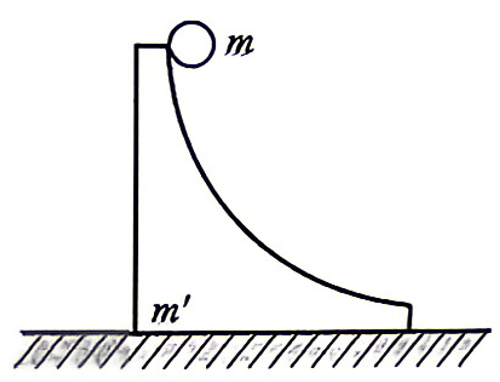
\includegraphics[width=0.3\linewidth]{figure/2-38}
	\caption{习题2-38图}
	\label{fig:2-38}
\end{figure}

\end{enumerate}


\subsection*{习题2题解}

\textbf{2-5题解：}
\setcounter{equation}{0}
\renewcommand{\theHequation}{2-5.\arabic{equation}}

\textbf{答案：} B

\textbf{解答过程：}
已知质点运动学方程为 $x = 5t, y = 0.5t^2$。
对时间 $t$ 求导，分别得到速度的 $x$ 和 $y$ 方向分量，如公式（\ref{eq:2-5-1}）和公式（\ref{eq:2-5-2}）所示：
\begin{equation}\label{eq:2-5-1}
	v_x = \frac{dx}{dt} = 5
\end{equation}
\begin{equation}\label{eq:2-5-2}
	v_y = \frac{dy}{dt} = t
\end{equation}
结合公式（\ref{eq:2-5-1}）和公式（\ref{eq:2-5-2}），可推导出质点速率的平方表达式（\ref{eq:2-5-3}）：
\begin{equation}\label{eq:2-5-3}
	v^2 = v_x^2 + v_y^2 = 25 + t^2
\end{equation}
根据动能定理，外力做功等于质点动能的变化量，其基本形式如公式（\ref{eq:2-5-4}）：
\begin{equation}\label{eq:2-5-4}
	W = \Delta E_k = \frac{1}{2}mv_2^2 - \frac{1}{2}mv_1^2
\end{equation}
在 $t_1 = 2\text{ s}$ 时，由公式（\ref{eq:2-5-3}）得速率平方 $v_1^2 = 25 + 2^2 = 29$，初动能 $E_{k1} = \frac{1}{2} \times 0.5 \times 29 = 7.25\text{ J}$。
在 $t_2 = 4\text{ s}$ 时，同理得速率平方 $v_2^2 = 25 + 4^2 = 41$，末动能 $E_{k2} = \frac{1}{2} \times 0.5 \times 41 = 10.25\text{ J}$。
将初末动能代入公式（\ref{eq:2-5-4}），得到外力做的功：
$$W = 10.25 - 7.25 = 3\text{ J}$$

\textbf{易混淆知识点说明：}
求变力做功时，若已知运动学方程，优先考虑使用\textbf{动能定理}（$W = \Delta E_k$），这比先求加速度、再求力、最后积分求功的方法要简便得多。注意速度是矢量，动能与速率的平方相关，计算速率时必须综合 $x$ 和 $y$ 两个方向的速度分量。

\vspace{2em}

\textbf{2-8题解：}
\setcounter{equation}{0}
\renewcommand{\theHequation}{2-8.\arabic{equation}}

\textbf{答案：} $290\text{ J}$

\textbf{解答过程：}
质点沿 $x$ 轴做直线运动，受到与坐标相关的变力 $F = (4 + 5x)\mathbf{i}$。
根据变力做功的定义式 $W = \int_{x_1}^{x_2} F_x dx$，对力在位移区间上进行定积分得到公式（\ref{eq:2-8-1}）：
\begin{equation}\label{eq:2-8-1}
	W = \int_{0}^{10} (4 + 5x) dx = \left[ 4x + \frac{5}{2}x^2 \right]_{0}^{10}
\end{equation}
将上下限代入公式（\ref{eq:2-8-1}）进行计算，得出最终做功数值（\ref{eq:2-8-2}）：
\begin{equation}\label{eq:2-8-2}
	W = \left(4 \times 10 + 2.5 \times 10^2\right) - 0 = 40 + 250 = 290\text{ J}
\end{equation}

\textbf{易混淆知识点说明：}
对于坐标相关的变力做功问题，必须严格通过积分计算。切忌生搬硬套恒力做功公式或将初末位置的力简单求平均（虽然本题力随位移线性变化，恰好可用平均力，但积分法是普适的通法，不易踩坑）。

\vspace{2em}

\textbf{2-11题解：}
\setcounter{equation}{0}
\renewcommand{\theHequation}{2-11.\arabic{equation}}

\textbf{答案：} $12\text{ J}$

\textbf{解答过程：}
根据动能定理，合外力做的功等于动能的增量，建立公式（\ref{eq:2-11-1}）：
\begin{equation}\label{eq:2-11-1}
	W_{\text{总}} = \Delta E_k = 24\text{ J}
\end{equation}
合外力做的功也等于各个分力单独做功的代数和，由此得出总功分配公式（\ref{eq:2-11-2}）：
\begin{equation}\label{eq:2-11-2}
	W_{\text{总}} = W_1 + W_2
\end{equation}
已知其中一个恒力 $F_1$，它所做的功为力矢量与位移矢量的标量积（点乘），计算过程如公式（\ref{eq:2-11-3}）：
\begin{equation}\label{eq:2-11-3}
	W_1 = \mathbf{F}_1 \cdot \Delta\mathbf{r} = (12\mathbf{i} - 3\mathbf{j}) \cdot (3\mathbf{i} + 8\mathbf{j}) = 12 \times 3 + (-3) \times 8 = 36 - 24 = 12\text{ J}
\end{equation}
将公式（\ref{eq:2-11-1}）和公式（\ref{eq:2-11-3}）的结果代入公式（\ref{eq:2-11-2}）中，推导出另一个恒力所做的功（\ref{eq:2-11-4}）：
\begin{equation}\label{eq:2-11-4}
	W_2 = W_{\text{总}} - W_1 = 24 - 12 = 12\text{ J}
\end{equation}

\textbf{易混淆知识点说明：}
功是标量，在进行矢量点乘运算 $\mathbf{A} \cdot \mathbf{B} = A_x B_x + A_y B_y$ 时，只需将对应的坐标分量相乘后再相加。计算时一定要注意坐标前面的正负号，容易因为粗心导致符号错误。

\vspace{2em}

\textbf{2-15题解：}
\setcounter{equation}{0}
\renewcommand{\theHequation}{2-15.\arabic{equation}}

\textbf{解答过程：}
(1) 求速度随时间变化的函数：
根据牛顿第二定律，子弹受到的合外力仅为阻力 $F = -kv$。
由 $F = ma = m\frac{dv}{dt}$，建立运动微分方程（\ref{eq:2-15-1}）：
\begin{equation}\label{eq:2-15-1}
	m\frac{dv}{dt} = -kv
\end{equation}
对公式（\ref{eq:2-15-1}）分离变量并进行定积分，得到公式（\ref{eq:2-15-2}）：
\begin{equation}\label{eq:2-15-2}
	\int_{v_0}^{v} \frac{dv}{v} = \int_{0}^{t} -\frac{k}{m} dt
\end{equation}
$$\ln v - \ln v_0 = -\frac{k}{m}t \implies \ln\left(\frac{v}{v_0}\right) = -\frac{k}{m}t$$
解出对应的速度函数表达式（\ref{eq:2-15-3}）：
\begin{equation}\label{eq:2-15-3}
	v(t) = v_0 e^{-\frac{k}{m}t}
\end{equation}

(2) 求子弹进入沙土的最大深度：
当子弹速度减为 $0$ 时，所经过的路程即为最大深度 $x_{\text{max}}$。
利用微积分中的链式法则变换加速度式 $a = \frac{dv}{dt} = \frac{dv}{dx}\frac{dx}{dt} = v\frac{dv}{dx}$，代入动力学方程并分离变量，得出微分公式（\ref{eq:2-15-4}）：
\begin{equation}\label{eq:2-15-4}
	m v \frac{dv}{dx} = -kv \implies \frac{dv}{dx} = -\frac{k}{m}
\end{equation}
将速度的上下限（$v_0 \to 0$）和位移的上下限（$0 \to x_{\text{max}}$）代入公式（\ref{eq:2-15-4}）进行积分：
$$\int_{v_0}^{0} dv = \int_{0}^{x_{\text{max}}} -\frac{k}{m} dx$$
$$0 - v_0 = -\frac{k}{m} x_{\text{max}}$$
由此推导出最大深度的最终结果（\ref{eq:2-15-5}）：
\begin{equation}\label{eq:2-15-5}
	x_{\text{max}} = \frac{mv_0}{k}
\end{equation}

\textbf{易混淆知识点说明：}
在解答第(2)问时，利用\textbf{链式求导法则} $\frac{dv}{dt} = v\frac{dv}{dx}$ 将包含“时间元”的微分方程转换为包含“空间元”的微分方程，是处理动力学中“求速度与位置的关系”或“求极限距离”问题最直接、最高效的技巧，可避免复杂的指数函数反解和无穷积分。

\vspace{2em}

\textbf{2-17题解：}
\setcounter{equation}{0}
\renewcommand{\theHequation}{2-17.\arabic{equation}}

\textbf{解答过程：}
已知质点质量 $m = 2\text{ kg}$，所受合外力 $\mathbf{F} = 4\mathbf{i} - 24t^2\mathbf{j}$。
由牛顿第二定律，推导出质点的加速度矢量公式（\ref{eq:2-17-1}）：
\begin{equation}\label{eq:2-17-1}
	\mathbf{a} = \frac{\mathbf{F}}{m} = 2\mathbf{i} - 12t^2\mathbf{j}
\end{equation}
速度是加速度对时间的积分（加上初速度），根据公式（\ref{eq:2-17-1}）进行积分得到速度函数（\ref{eq:2-17-2}）：
\begin{equation}\label{eq:2-17-2}
	\mathbf{v}(t) = \mathbf{v}_0 + \int_{0}^{t} \mathbf{a} dt = (3\mathbf{i} + 4\mathbf{j}) + \int_{0}^{t} (2\mathbf{i} - 12t^2\mathbf{j}) dt
\end{equation}
$$\mathbf{v}(t) = (3\mathbf{i} + 4\mathbf{j}) + (2t\mathbf{i} - 4t^3\mathbf{j}) = (3 + 2t)\mathbf{i} + (4 - 4t^3)\mathbf{j}$$
将 $t = 1\text{ s}$ 代入，得出该特定时刻的速度（\ref{eq:2-17-3}）：
\begin{equation}\label{eq:2-17-3}
	\mathbf{v}(1) = (3 + 2 \times 1)\mathbf{i} + (4 - 4 \times 1^3)\mathbf{j} = 5\mathbf{i} + 0\mathbf{j} = 5\mathbf{i}\text{ (m/s)}
\end{equation}
同时，代入 $t = 1\text{ s}$ 计算此时质点受到的总力矢量（\ref{eq:2-17-4}）：
\begin{equation}\label{eq:2-17-4}
	\mathbf{F}(1) = 4\mathbf{i} - 24(1)^2\mathbf{j} = 4\mathbf{i} - 24\mathbf{j}\text{ (N)}
\end{equation}
法向力 $\mathbf{F}_n$ 是\textbf{合外力中与此时速度方向垂直的分量}。
由公式（\ref{eq:2-17-3}）可知，在 $t = 1\text{ s}$ 时，速度 $\mathbf{v} = 5\mathbf{i}$ 的方向仅沿 $x$ 轴。
结合公式（\ref{eq:2-17-4}），总力的 $x$ 轴分量 $4\mathbf{i}$ 是\textbf{平行于速度的切向力}，而力的 $y$ 轴分量 $-24\mathbf{j}$ 则是\textbf{垂直于速度的法向力}。
因此，质点受到的法向力矢量为 $\mathbf{F}_n = -24\mathbf{j}\text{ N}$\textbf{（其大小为 $24\text{ N}$）}。

\textbf{易混淆知识点说明：}
法向力和切向力是相对\textbf{瞬时速度方向}而定义的。切不可主观地认为 $\mathbf{i}$ 方向就是切向、$\mathbf{j}$ 方向就是法向。必须先求解出具体时刻的\textbf{速度矢量}，然后将该时刻的合外力正交分解为平行于速度方向的分量（切向力）和垂直于速度方向的分量（法向力）。本题恰好在 $t=1\text{ s}$ 时刻速度纯沿 $x$ 轴，才使得分解如此直观。

\vspace{2em}

\textbf{2-25题解：}
\setcounter{equation}{0}
\renewcommand{\theHequation}{2-25.\arabic{equation}}

\textbf{解答过程：}
(1) 求子弹走完枪筒全长所需时间：
已知子弹受到的合力为 $F = a - bt$。
假设子弹运动到枪口处合力刚好为零，建立受力终点方程（\ref{eq:2-25-1}）：
\begin{equation}\label{eq:2-25-1}
	F(t) = a - bt = 0
\end{equation}
由公式（\ref{eq:2-25-1}）解得子弹在枪筒内运动的总时间 $t = \frac{a}{b}$。

(2) 求子弹所受的冲量：
根据冲量的定义式 $I = \int F dt$，在时间区间 $[0, \frac{a}{b}]$ 内对合力进行定积分，得到公式（\ref{eq:2-25-2}）：
\begin{equation}\label{eq:2-25-2}
	I = \int_{0}^{\frac{a}{b}} (a - bt) dt = \left[ at - \frac{1}{2}bt^2 \right]_{0}^{\frac{a}{b}}
\end{equation}
将上下限代入公式（\ref{eq:2-25-2}）进行计算，得出总冲量表达式（\ref{eq:2-25-3}）：
\begin{equation}\label{eq:2-25-3}
	I = a\left(\frac{a}{b}\right) - \frac{1}{2}b\left(\frac{a}{b}\right)^2 = \frac{a^2}{b} - \frac{a^2}{2b} = \frac{a^2}{2b}
\end{equation}

(3) 求子弹的质量：
根据动量定理，合外力的冲量等于子弹动量的变化量，由此建立公式（\ref{eq:2-25-4}）：
\begin{equation}\label{eq:2-25-4}
	I = \Delta p = mv_0 - m(0) = mv_0
\end{equation}
将公式（\ref{eq:2-25-3}）求得的冲量结果代入公式（\ref{eq:2-25-4}）中：
$$\frac{a^2}{2b} = mv_0$$
最后解出子弹的质量解析式（\ref{eq:2-25-5}）：
\begin{equation}\label{eq:2-25-5}
	m = \frac{a^2}{2bv_0}
\end{equation}

\textbf{易混淆知识点说明：}
本题容易混淆空间积分与时间积分。题目给定的力是\textbf{时间的函数}，所以求冲量必须用时间积分 $I = \int F dt$；如果求功，才是对空间位移的积分。动量定理建立了时间累积效应（冲量）与状态量变化（动量变化）之间的桥梁。

\vspace{2em}

\textbf{2-29题解：}
\setcounter{equation}{0}
\renewcommand{\theHequation}{2-29.\arabic{equation}}

\textbf{解答过程：}
已知质点所受合力矢量 $\mathbf{F}_{\text{合}} = (7\mathbf{i} - 6\mathbf{j})\text{ N}$。
(1) 求合力所做的功：
质点从原点 $(0,0,0)$ 运动到 $\mathbf{r} = (-3\mathbf{i} + 4\mathbf{j} + 16\mathbf{k})\text{ m}$，位移矢量即为位置矢量本身：$\Delta\mathbf{r} = -3\mathbf{i} + 4\mathbf{j} + 16\mathbf{k}$。
恒力做功等于力矢量与位移矢量的点乘（数量积），计算如公式（\ref{eq:2-29-1}）：
\begin{equation}\label{eq:2-29-1}
	W = \mathbf{F}_{\text{合}} \cdot \Delta\mathbf{r} = (7\mathbf{i} - 6\mathbf{j} + 0\mathbf{k}) \cdot (-3\mathbf{i} + 4\mathbf{j} + 16\mathbf{k})
\end{equation}
$$W = 7 \times (-3) + (-6) \times 4 + 0 \times 16 = -21 - 24 = -45\text{ J}$$

(2) 求合力做功的平均功率：
平均功率定义为功除以时间，将上一步计算的功代入公式（\ref{eq:2-29-2}）：
\begin{equation}\label{eq:2-29-2}
	\bar{P} = \frac{W}{t} = \frac{-45\text{ J}}{0.6\text{ s}} = -75\text{ W}
\end{equation}

(3) 求质点动能的变化：
根据动能定理，合外力对质点做的总功等于质点动能的变化量，由此推出关系式（\ref{eq:2-29-3}）：
\begin{equation}\label{eq:2-29-3}
	\Delta E_k = W_{\text{合}} = -45\text{ J}
\end{equation}
（动能减少了 $45\text{ J}$）

\textbf{易混淆知识点说明：}
在进行矢量点积计算时，必须是对应坐标系（$\mathbf{i}, \mathbf{j}, \mathbf{k}$）的系数相乘再相加。力只有 $\mathbf{i}$ 和 $\mathbf{j}$ 方向的分量，所以位移中 $\mathbf{k}$ 方向的移动不产生功。另外，功和动能变化量\textbf{可以是负值}，表示外界对系统做负功，系统动能减少。

\vspace{2em}

\textbf{2-31题解：}
\setcounter{equation}{0}
\renewcommand{\theHequation}{2-31.\arabic{equation}}

\textbf{答案：} $980\text{ J}$ （取 $g=9.8\text{ m/s}^2$）或 $1000\text{ J}$ （取 $g=10\text{ m/s}^2$），以下过程以重力加速度 $g$ 符号保留，最后代入标准值 $9.8\text{ m/s}^2$。

\textbf{解答过程：}
这是一个变力做功的问题。因为水桶在匀速上升过程中不断漏水，所以水桶和水的总质量 $m$ 是高度 $y$（距水面的高度）的函数。
设水桶上升高度为 $y$ 时的总质量为 $M(y)。$
已知空桶质量 $m_{\text{桶}} = 1\text{ kg}$，初始水质量 $m_{\text{水0}} = 10\text{ kg}$，每升高 $1\text{ m}$ 漏水 $0.2\text{ kg}$。
在高度 $y$ 处，剩下的水质量为 $m_{\text{水}}(y) = 10 - 0.2y$。
总质量 $M(y) = 1 + (10 - 0.2y) = 11 - 0.2y$。
因为是匀速提升，人施加的拉力大小等于总重力，由此得出受力函数公式（\ref{eq:2-31-1}）：
\begin{equation}\label{eq:2-31-1}
	F(y) = M(y)g = (11 - 0.2y)g
\end{equation}
人做功微元为 $dW = F(y) dy$，对整个高度 $y \in [0, 10]$ 进行定积分得到总功的计算公式（\ref{eq:2-31-2}）：
\begin{equation}\label{eq:2-31-2}
	W = \int_{0}^{10} F(y) dy = \int_{0}^{10} (11 - 0.2y)g dy
\end{equation}
$$W = g \left[ 11y - \frac{0.2}{2}y^2 \right]_{0}^{10} = g \left[ 11y - 0.1y^2 \right]_{0}^{10}$$
代入上下限：
$$W = g (11 \times 10 - 0.1 \times 100) = g(110 - 10) = 100g$$
将 $g = 9.8\text{ m/s}^2$ 代入，则人做的最终总功为公式（\ref{eq:2-31-3}）：
\begin{equation}\label{eq:2-31-3}
	W = 100 \times 9.8 = 980\text{ J}
\end{equation}

\textbf{易混淆知识点说明：}
处理质量随位移变化的系统时，绝不能直接用“初态重力”或“末态重力”乘以总高度，也不能简单地用平均质量来套用 $W = mgh$（虽然本题恰好线性变化，平均质量计算结果也对，但积分法是正统且不限函数的通用解法）。必须写出\textbf{力随位移的函数}并进行定积分运算。

\vspace{2em}

\textbf{2-38题解：}
\setcounter{equation}{0}
\renewcommand{\theHequation}{2-38.\arabic{equation}}

\textbf{解答过程：}
小球 $m$ 从木块 $m'$ 的四分之一圆弧槽滑下的过程中，由于地面光滑（无摩擦），系统在\textbf{水平方向}上不受外力，因此水平方向动量守恒。同时，系统只有重力做功，系统\textbf{机械能守恒}。
设小球脱离大木块时，小球相对于地面的速度大小为 $v$，方向水平向左；大木块相对于地面的速度大小为 $V$，方向水平向右。\\
1. 水平方向动量守恒（以小球速度方向为正），建立守恒公式（\ref{eq:2-38-1}）：
\begin{equation}\label{eq:2-38-1}
	mv - m'V = 0 \implies V = \frac{m}{m'}v
\end{equation}
2. 系统机械能守恒（以小球初位置为零势能面或利用势能减少等于动能增加），建立能量转化公式（\ref{eq:2-38-2}）：
\begin{equation}\label{eq:2-38-2}
	mgR = \frac{1}{2}mv^2 + \frac{1}{2}m'V^2
\end{equation}
将由公式（\ref{eq:2-38-1}）解出的 $V$ 代入公式（\ref{eq:2-38-2}）的机械能守恒方程中，推导出代入后的表达式（\ref{eq:2-38-3}）：
\begin{equation}\label{eq:2-38-3}
	mgR = \frac{1}{2}mv^2 + \frac{1}{2}m'\left(\frac{m}{m'}v\right)^2 = \frac{1}{2}mv^2 + \frac{1}{2}\frac{m^2}{m'}v^2
\end{equation}
对公式（\ref{eq:2-38-3}）的右侧提取公因式 $\frac{1}{2}mv^2$ 并通分：
$$mgR = \frac{1}{2}mv^2 \left(1 + \frac{m}{m'}\right) = \frac{1}{2}mv^2 \left(\frac{m' + m}{m'}\right)$$
消去等式两边的一个 $m$ 并解出 $v^2$：
$$v^2 = \frac{2gR \cdot m'}{m + m'}$$
对两边开平方，由公式（\ref{eq:2-38-1}）和（\ref{eq:2-38-2}）最终联合推出小球脱离大木块时的速度公式（\ref{eq:2-38-4}）：
\begin{equation}\label{eq:2-38-4}
	v = \sqrt{\frac{2m'gR}{m + m'}}
\end{equation}

\textbf{易混淆知识点说明：}
很多学生看到“四分之一光滑圆弧槽”会习惯性地直接套用 $v = \sqrt{2gR}$。\textcolor{red}{必须注意}，那是木块\textbf{固定在地面上}的情况。本题大木块放在光滑水平面上，小球下滑的同时，木块也会向相反方向后退，因此重力势能不仅转化为小球的动能，还转化为了大木块的动能。解决包含可移动斜面/曲面的相互作用问题时，核心武器是\textbf{“水平动量守恒 + 系统机械能守恒”}联立求解。
\newpage

\subsection{习题3}
\begin{enumerate}

\item[\textbf{3-10}]
固定在一起的两个同轴均匀圆柱体可绕其光滑的水平对称轴 \(OO'\) 转动.设大小圆柱体的半径分别为 \(R\) 和 \(r\),质量分别为 \(m'\) 和 \(m\).绕在两柱体上的细绳分别与物体 \(m_1\) 和 \(m_2\) 相连,\(m_1\) 和 \(m_2\) 则挂在圆柱体的两侧,如习题 3-10 图所示.设 \(R=0.20\,\mathrm{m}\),\(r=0.10\,\mathrm{m}\),\(m=4\,\mathrm{kg}\),\(m'=10\,\mathrm{kg}\),\(m_1=m_2=2\,\mathrm{kg}\),且开始时 \(m_1\) 和 \(m_2\) 离地高度均为 \(h=2\,\mathrm{m}\).


\begin{figure}[H]
	\centering
	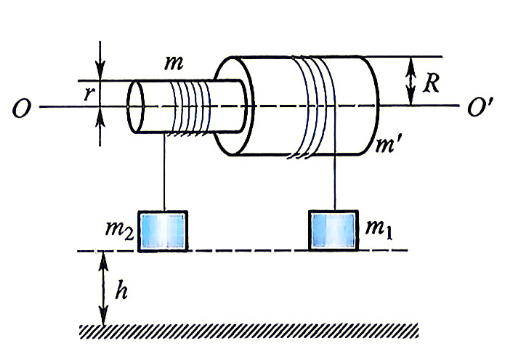
\includegraphics[width=0.3\linewidth]{figure/3-10}
	\caption{习题3-10图}
	\label{fig:3-10}
\end{figure}


\begin{enumerate}
	\item 求柱体转动时的角加速度；
	\item 求两侧细绳的张力；
	\item $m_1$ 和 $m_2$ 哪个先落地？它落地前瞬间的速率为多少？
\end{enumerate}

\item[\textbf{3-11}]
计算如习题 3-11 图所示系统中物体的加速度大小.设滑轮为质量均匀分布的圆柱体,半径为 \(r=0.1\,\mathrm{m}\),轻绳不可伸长,且与滑轮之间无相对滑动,滑轮轴上摩擦不计,且忽略桌面与物体 \(m_1\) 间的摩擦,已知 \(m_1=50\,\mathrm{kg}\),\(m_2=200\,\mathrm{kg}\),滑轮质量 \(m'=15\,\mathrm{kg}\).

\begin{figure}[H]
	\centering
	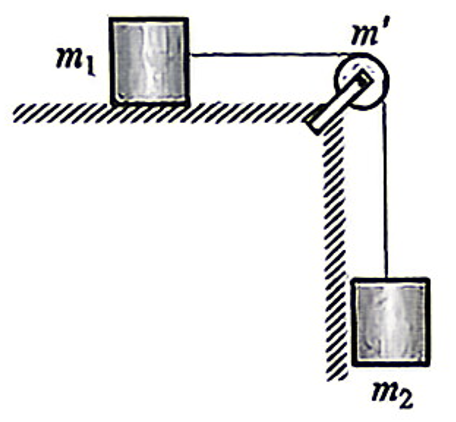
\includegraphics[width=0.3\linewidth]{figure/3-11}
	\caption{习题3-11图}
	\label{fig:3-11}
\end{figure}


\item[\textbf{3-12}]
如习题 3-12 图所示,一匀质细杆质量为 \(m\),长为 \(l\),可绕过一端 \(O\) 的水平光滑固定轴转动,杆从水平位置由静止开始摆下.求:
\begin{enumerate}
	\item 初始时刻的角加速度；
	\item 杆转过 \(\theta\) 角时的角加速度和角速度.
\end{enumerate}

\begin{figure}[H]
	\centering
	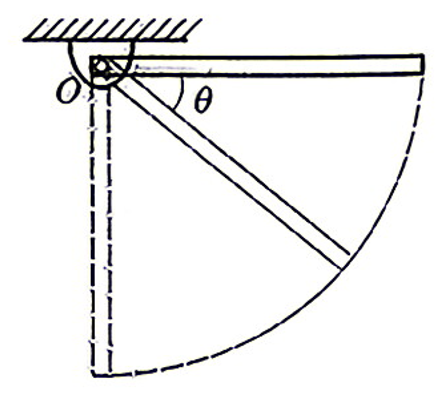
\includegraphics[width=0.3\linewidth]{figure/3-12}
	\caption{习题3-12图}
	\label{fig:3-12}
\end{figure}


\item[\textbf{3-13}]
如习题 3-13 图所示,一长为 \(1\,\mathrm{m}\) 的均匀直棒可绕其一端与棒垂直的水平光滑固定轴转动,抬起另一端使棒向上与水平面成 \(60^\circ\) 角,然后无初速度地将棒释放,求:
\begin{enumerate}
	\item 放手时棒的角加速度；
	\item 棒转到竖直位置时的角速度.
\end{enumerate}

\begin{figure}[H]
	\centering
	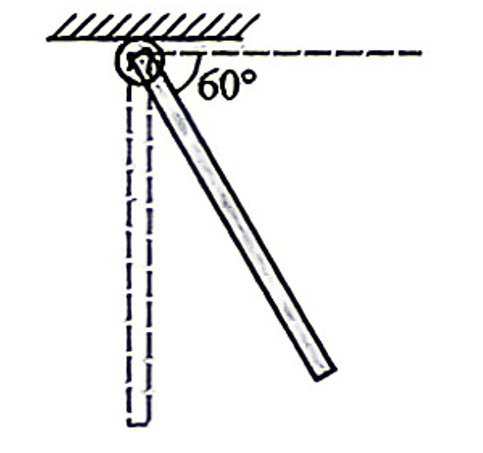
\includegraphics[width=0.3\linewidth]{figure/3-13}
	\caption{习题3-13图}
	\label{fig:3-13}
\end{figure}


\item[\textbf{3-14}]
如习题 3-14 图所示,长为 \(L\)、质量为 \(m\) 的均匀细杆静止在水平桌面上,可绕通过左端 \(O\) 点的竖直光滑轴转动.一质量为 \(m_0=m/3\) 的小球以速度 \(v_0\) 垂直击杆于 \(P\) 点,并以速度 \(v=v_0/3\) 弹回.设 \(OP=(3/4)L\),杆与水平面间的摩擦系数为 \(\mu\).求:
\begin{enumerate}
	\item 开始转动时的角速度；
	\item 杆所受摩擦力矩的大小；
	\item 杆从开始转动到静止所转过的角度和经历的时间.
\end{enumerate}

\begin{figure}[H]
	\centering
	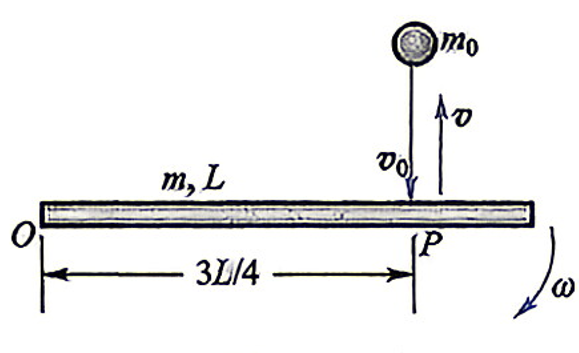
\includegraphics[width=0.3\linewidth]{figure/3-14}
	\caption{习题3-14图}
	\label{fig:3-14}
\end{figure}

\item[\textbf{3-16}]
有一质量为 \(m_1\)、长为 \(l\) 的均匀的细棒 \(OA\),可绕一端的水平固定轴 \(O\) 自由转动,初始时静止悬挂.一水平运动的质量为 \(m_2\) 的小球,从侧面垂直于棒和轴与棒的另一端 \(A\) 相碰撞,设碰撞时间极短.已知小球在碰撞前后的速度分别为 \(v_1\)、\(v_2\),方向如习题 3-16 图所示.求:
\begin{enumerate}
	\item 碰撞后瞬间细棒的角速度；
	\item 细棒能够摆动的最大摆角 \(\theta_m\).
\end{enumerate}

\begin{figure}[H]
	\centering
	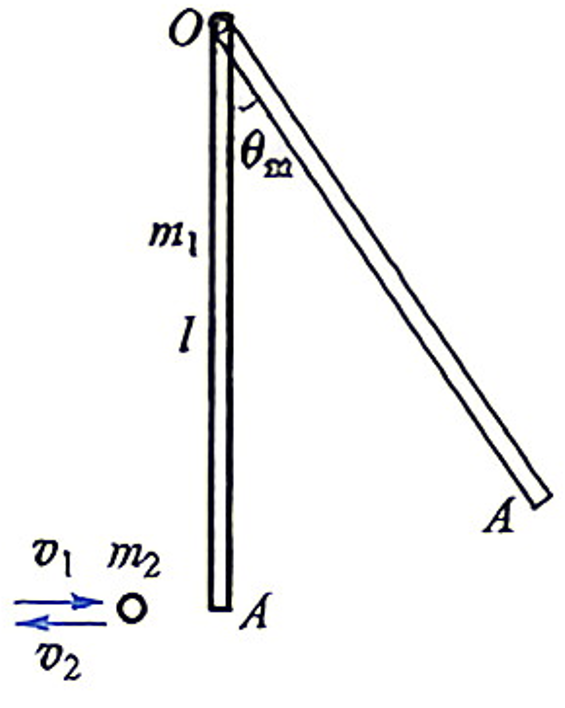
\includegraphics[width=0.3\linewidth]{figure/3-16}
	\caption{习题3-16图}
	\label{fig:3-16}
\end{figure}


\item[\textbf{3-17}]
如习题 3-17 图所示,一长为 \(l\)、质量为 \(m_1\) 的均质细杆,可绕通过其一端的水平轴 \(O\) 在竖直平面内自由转动,杆从水平位置由静止释放后,与 \(O\) 点正下方静止在光滑水平面上的物体 \(m_2\) 发生碰撞,\(m_2=m_1/3\).求:
\begin{enumerate}
	\item 杆在转动过程中 \(\theta\) 角加速度 \(\alpha\) 的表达式；
	\item 杆转到竖直位置时的角动量和动能；
	\item 若碰撞是完全弹性的,碰撞后 \(m_2\) 的速度；
	\item 弹簧被压缩的最大长度.
\end{enumerate}

\begin{figure}[H]
	\centering
	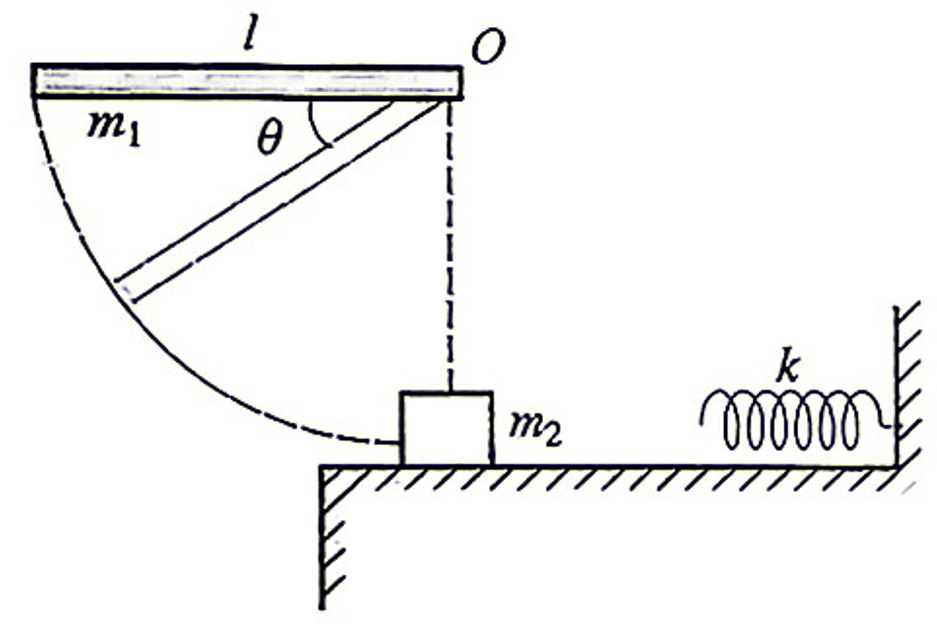
\includegraphics[width=0.3\linewidth]{figure/3-17}
	\caption{习题3-17图}
	\label{fig:3-17}
\end{figure}

\end{enumerate}

\subsection*{习题3题解}

\textbf{3-10题解：}
\setcounter{equation}{0}
\renewcommand{\theHequation}{3-10.\arabic{equation}}

\textbf{解答过程：}
\textbf{计算由两个同轴圆柱体组成的刚体系统的总转动惯量 $J$:}
大圆柱体的转动惯量与小圆柱体的转动惯量之和由公式（\ref{eq:3-10-1}）表示：
\begin{equation}\label{eq:3-10-1}
	J = \frac{1}{2}m'R^2 + \frac{1}{2}mr^2
\end{equation}
代入已知数据 $R = 0.20 \text{ m}, r = 0.10 \text{ m}, m = 4 \text{ kg}, m' = 10 \text{ kg}$，计算出转动惯量如公式（\ref{eq:3-10-2}）：
\begin{equation}\label{eq:3-10-2}
	J = \frac{1}{2} \times 10 \times (0.20)^2 + \frac{1}{2} \times 4 \times (0.10)^2 = 0.22 \text{ kg}\cdot\text{m}^2
\end{equation}

设系统的角加速度为 $\alpha$（设 $m_1$ 下降方向对应转动正方向），$m_1$ 向下的加速度为 $a_1$，$m_2$ 向上的加速度为 $a_2$。两侧细绳的张力分别为 $T_1$ 和 $T_2$。
根据刚体转动与平动的运动学关系，建立公式（\ref{eq:3-10-3}）和公式（\ref{eq:3-10-4}）：
\begin{equation}\label{eq:3-10-3}
	a_1 = \alpha R
\end{equation}
\begin{equation}\label{eq:3-10-4}
	a_2 = \alpha r
\end{equation}

(1). \textbf{求柱体转动时的角加速度 $\alpha$：}
对 $m_1$ 应用牛顿第二定律（向下为正），结合公式（\ref{eq:3-10-3}）得到公式（\ref{eq:3-10-5}）：
\begin{equation}\label{eq:3-10-5}
	m_1 g - T_1 = m_1 a_1 \implies T_1 = m_1(g - \alpha R)
\end{equation}
对 $m_2$ 应用牛顿第二定律（向上为正），结合公式（\ref{eq:3-10-4}）得到公式（\ref{eq:3-10-6}）：
\begin{equation}\label{eq:3-10-6}
	T_2 - m_2 g = m_2 a_2 \implies T_2 = m_2(g + \alpha r)
\end{equation}
对转动系统应用刚体定轴转动定律，建立公式（\ref{eq:3-10-7}）：
\begin{equation}\label{eq:3-10-7}
	T_1 R - T_2 r = J \alpha
\end{equation}
将公式（\ref{eq:3-10-5}）和公式（\ref{eq:3-10-6}）代入公式（\ref{eq:3-10-7}）中，得到公式（\ref{eq:3-10-8}）：
\begin{equation}\label{eq:3-10-8}
	m_1(g - \alpha R)R - m_2(g + \alpha r)r = J \alpha
\end{equation}
将公式（\ref{eq:3-10-8}）展开并提取出 $\alpha$，推导出角加速度的表达式（\ref{eq:3-10-9}）：
\begin{equation}\label{eq:3-10-9}
	\alpha = \frac{(m_1 R - m_2 r)g}{J + m_1 R^2 + m_2 r^2}
\end{equation}
将公式（\ref{eq:3-10-2}）的结果和已知数据代入公式（\ref{eq:3-10-9}）中（取 $g = 9.8 \text{ m/s}^2$，$m_1 = m_2 = 2 \text{ kg}$）：
\begin{equation}\label{eq:3-10-10}
	\alpha = \frac{(2 \times 0.20 - 2 \times 0.10) \times 9.8}{0.22 + 2 \times 0.20^2 + 2 \times 0.10^2} = \frac{1.96}{0.32} = 6.125 \text{ rad/s}^2
\end{equation}

(2). \textbf{求两侧细绳的张力：}
将由公式（\ref{eq:3-10-10}）求得的 $\alpha$ 分别代回公式（\ref{eq:3-10-5}）和公式（\ref{eq:3-10-6}），得出张力公式（\ref{eq:3-10-11}）和公式（\ref{eq:3-10-12}）：
\begin{equation}\label{eq:3-10-11}
	T_1 = m_1(g - \alpha R) = 2 \times (9.8 - 6.125 \times 0.20) = 17.15 \text{ N}
\end{equation}
\begin{equation}\label{eq:3-10-12}
	T_2 = m_2(g + \alpha r) = 2 \times (9.8 + 6.125 \times 0.10) = 20.825 \text{ N}
\end{equation}

(3). \textbf{判断哪个先落地及落地前瞬间的速率：}
由于 $m_1$ 产生的力矩 $m_1 g R > m_2 g r$，系统将顺时针加速转动，$m_1$ 加速下降而 $m_2$ 加速上升，且初始高度相同，因此 **$m_1$ 先落地**。
$m_1$ 下落时的恒定线加速度由公式（\ref{eq:3-10-3}）得 $a_1 = \alpha R = 6.125 \times 0.20 = 1.225 \text{ m/s}^2$。
根据匀变速直线运动规律，初速度为 $0$，位移 $h = 2 \text{ m}$，落地速率 $v_1$ 满足公式（\ref{eq:3-10-13}）：
\begin{equation}\label{eq:3-10-13}
	v_1^2 = 2 a_1 h \implies v_1 = \sqrt{2 \times 1.225 \times 2}
\end{equation}
由公式（\ref{eq:3-10-13}）解得 $m_1$ 落地前瞬间的速率（\ref{eq:3-10-14}）：
\begin{equation}\label{eq:3-10-14}
	v_1 = \sqrt{4.9} \approx 2.21 \text{ m/s}
\end{equation}

\vspace{1em}

\textbf{易混淆知识点说明：}
1. \textbf{角加速度与线加速度的对应关系：} 极易犯错的地方在于把两物体的加速度设为同一个 $a$。由于 $m_1$ 和 $m_2$ 悬挂在不同半径的圆柱上，它们的线位移、线速度和线加速度均不相同，必须通过各自的半径与系统的角加速度联系起来（即 $a_1 = \alpha R$ 和 $a_2 = \alpha r$）。

2. \textbf{加速系统中的张力计算：} 很多学生习惯性地认为绳子张力等于物体重力（$T=mg$）。实际上，只有在物体静止或匀速直线运动时才成立。对于有加速度的系统，张力必定大于（上升时）或小于（下降时）物体的重力，必须严格通过隔离法列牛顿第二定律方程来求解。

3. \textbf{转动惯量的叠加性：} 处理复合刚体（如本题中的阶梯形圆柱体）时，其相对于同一转轴的总转动惯量，直接等于各部分转动惯量的代数和。

\vspace{2em}

\textbf{3-11题解：}
\setcounter{equation}{0}
\renewcommand{\theHequation}{3-11.\arabic{equation}}

\textbf{解答过程：}
设系统物体的加速度大小为 $a$，滑轮的角加速度为 $\alpha$。
两侧细绳的张力分别设为 $T_1$（连接 $m_1$ 侧）和 $T_2$（连接 $m_2$ 侧）。

对水平桌面上的物体 $m_1$（忽略摩擦），在水平方向应用牛顿第二定律建立公式（\ref{eq:3-11-1}）：
\begin{equation}\label{eq:3-11-1}
	T_1 = m_1 a
\end{equation}

对悬挂的物体 $m_2$，在竖直方向应用牛顿第二定律（设向下为正方向）建立公式（\ref{eq:3-11-2}）：
\begin{equation}\label{eq:3-11-2}
	m_2 g - T_2 = m_2 a
\end{equation}

对具有质量的定滑轮，应用刚体定轴转动定律建立公式（\ref{eq:3-11-3}）：
\begin{equation}\label{eq:3-11-3}
	(T_2 - T_1)r = J\alpha
\end{equation}

其中，质量均匀分布的圆柱体（滑轮）的转动惯量 $J$ 如公式（\ref{eq:3-11-4}）：
\begin{equation}\label{eq:3-11-4}
	J = \frac{1}{2}m'r^2
\end{equation}

绳子不可伸长且与滑轮之间无相对滑动，线加速度与角加速度的运动学关系如公式（\ref{eq:3-11-5}）：
\begin{equation}\label{eq:3-11-5}
	a = \alpha r
\end{equation}

将公式（\ref{eq:3-11-4}）和公式（\ref{eq:3-11-5}）代入公式（\ref{eq:3-11-3}）中，消去 $J$ 和 $\alpha$，得到关于线加速度的转动方程（\ref{eq:3-11-6}）：
\begin{equation}\label{eq:3-11-6}
	(T_2 - T_1)r = \left(\frac{1}{2}m'r^2\right) \left(\frac{a}{r}\right) \implies T_2 - T_1 = \frac{1}{2}m'a
\end{equation}

将公式（\ref{eq:3-11-1}）中的 $T_1$ 和公式（\ref{eq:3-11-2}）变形得到的 $T_2 = m_2 g - m_2 a$ 一并代入公式（\ref{eq:3-11-6}）中：
\begin{equation}\label{eq:3-11-7}
	(m_2 g - m_2 a) - m_1 a = \frac{1}{2}m'a
\end{equation}

对公式（\ref{eq:3-11-7}）移项并提取公因式 $a$，解得系统加速度的一般表达式（\ref{eq:3-11-8}）：
\begin{equation}\label{eq:3-11-8}
	a = \frac{m_2 g}{m_1 + m_2 + \frac{1}{2}m'}
\end{equation}

代入已知数据 $m_1 = 50\text{ kg}, m_2 = 200\text{ kg}, m' = 15\text{ kg}$，取重力加速度 $g = 9.8\text{ m/s}^2$ 得到最终结果（\ref{eq:3-11-9}）：
\begin{equation}\label{eq:3-11-9}
	a = \frac{200 \times 9.8}{50 + 200 + \frac{1}{2} \times 15} = \frac{1960}{257.5} \approx 7.61 \text{ m/s}^2
\end{equation}
\textcolor{red}{（注：若题目要求取 $g = 10\text{ m/s}^2$，代入上式计算得 $a \approx 7.77\text{ m/s}^2$）}

\vspace{1em}

\textbf{易混淆知识点说明：}
处理带有质量的定滑轮系统时，\textbf{绝不能}像基础质点力学中那样假设“同一根轻绳两端张力处处相等”（即认为 $T_1 = T_2$）。滑轮有质量就意味着其具有转动惯量，绳子对滑轮两侧的张力必然存在差值，正是这个差值产生的合力矩 $(T_2 - T_1)r$ 提供了滑轮加速转动所需的动力。因此，必须依次建立两个平动方程、一个转动方程和一个线角关联方程，然后联立求解。

\vspace{2em}

\textbf{3-12题解：}
\setcounter{equation}{0}
\renewcommand{\theHequation}{3-12.\arabic{equation}}

\textbf{解答过程：}
细杆可绕过端点 $O$ 的水平固定轴转动，这是一个典型的刚体定轴转动问题。
根据刚体转动惯量的计算，均匀细杆绕过其一端且垂直于杆的轴的转动惯量 $J$ 为公式（\ref{eq:3-12-1}）：
\begin{equation}\label{eq:3-12-1}
	J = \frac{1}{3}ml^2
\end{equation}

(1) \textbf{求初始时刻的角加速度 $\alpha_0$：}
初始时刻，细杆处于静止的水平位置。此时重力 $mg$ 集中作用在杆的质心（距 $O$ 点距离为 $\frac{l}{2}$）上。此时重力的力臂最大，产生的重力力矩 $\tau_0$ 见公式（\ref{eq:3-12-2}）：
\begin{equation}\label{eq:3-12-2}
	\tau_0 = mg \frac{l}{2}
\end{equation}
根据刚体定轴转动定律 $\tau = J\alpha$，结合公式（\ref{eq:3-12-1}）和公式（\ref{eq:3-12-2}）可得初始时刻的角加速度算式（\ref{eq:3-12-3}）：
\begin{equation}\label{eq:3-12-3}
	\alpha_0 = \frac{\tau_0}{J} = \frac{mg \frac{l}{2}}{\frac{1}{3}ml^2}
\end{equation}
化简公式（\ref{eq:3-12-3}），得到初始时刻的角加速度表达式（\ref{eq:3-12-4}）：
\begin{equation}\label{eq:3-12-4}
	\alpha_0 = \frac{3g}{2l}
\end{equation}

(2) \textbf{求杆转过 $\theta$ 角时的角加速度 $\alpha$ 和角速度 $\omega$：}
当细杆从水平位置向下转过 $\theta$ 角时，根据题图可知，$\theta$ 为杆与水平线的夹角。此时质心到 $O$ 点的水平距离（即重力力臂）减小为 $\frac{l}{2} \cos\theta$。
此时重力产生的力矩 $\tau$ 为公式（\ref{eq:3-12-5}）：
\begin{equation}\label{eq:3-12-5}
	\tau = mg \frac{l}{2} \cos\theta
\end{equation}
再次应用刚体定轴转动定律 $\tau = J\alpha$，结合公式（\ref{eq:3-12-1}）和公式（\ref{eq:3-12-5}），得到此时的角加速度算式（\ref{eq:3-12-6}）：
\begin{equation}\label{eq:3-12-6}
	\alpha = \frac{\tau}{J} = \frac{mg \frac{l}{2} \cos\theta}{\frac{1}{3}ml^2}
\end{equation}
化简公式（\ref{eq:3-12-6}）得此时的角加速度（\ref{eq:3-12-7}）：
\begin{equation}\label{eq:3-12-7}
	\alpha = \frac{3g \cos\theta}{2l}
\end{equation}

为了求解角速度 $\omega$，最简便的方法是使用\textbf{机械能守恒定律}。
取细杆的初始水平位置为重力势能零势面，细杆从静止释放，初态总机械能 $E_1 = 0$。
当杆转过 $\theta$ 角时，杆的质心下降的垂直高度为 $h = \frac{l}{2} \sin\theta$。
根据机械能守恒定律，系统的重力势能与转动动能之和为零，建立公式（\ref{eq:3-12-8}）：
\begin{equation}\label{eq:3-12-8}
	0 = -mg \frac{l}{2} \sin\theta + \frac{1}{2}J\omega^2 
\end{equation}
对公式（\ref{eq:3-12-8}）移项并将公式（\ref{eq:3-12-1}）中的转动惯量代入：
\begin{equation}\label{eq:3-12-9}
	mg \frac{l}{2} \sin\theta = \frac{1}{2} \left(\frac{1}{3}ml^2\right) \omega^2
\end{equation}
进一步化简等式（\ref{eq:3-12-9}）：
\begin{equation}\label{eq:3-12-10}
	mg \frac{l}{2} \sin\theta = \frac{1}{6} ml^2 \omega^2 \implies 3g \sin\theta = l\omega^2
\end{equation}
对公式（\ref{eq:3-12-10}）中的 $\omega^2$ 开平方，解得此时的角速度大小（\ref{eq:3-12-11}）：
\begin{equation}\label{eq:3-12-11}
	\omega = \sqrt{\frac{3g \sin\theta}{l}}
\end{equation}

\vspace{1em}

\textbf{易混淆知识点说明：}
1. \textbf{转动惯量的选取：} 细杆绕\textbf{端点}转动的转动惯量是 $J = \frac{1}{3}ml^2$，而绕\textbf{质心}转动的转动惯量是 $J_c = \frac{1}{12}ml^2$。本题固定轴在 $O$ 点（端点），极易因为记忆模糊而错代为质心的转动惯量。

2. \textbf{重力力矩的力臂计算：} 在计算任意转角 $\theta$ 的重力力矩时，必须明确 $\theta$ 的几何定义。本题图中明确标识 $\theta$ 是杆与\textbf{水平线}的夹角，因此重力作用线的垂直距离（力臂）是 $\frac{l}{2}\cos\theta$；若某些题目中定义 $\theta$ 为与\textbf{竖直方向}的偏角，力臂则会变为 $\frac{l}{2}\sin\theta$。做此类转动问题时，仔细审图是保证力矩表达式正确的前提。

\vspace{2em}

\textbf{3-13题解：}
\setcounter{equation}{0}
\renewcommand{\theHequation}{3-13.\arabic{equation}}

\textbf{解答过程：}
(1). \textbf{求放手时棒的角加速度：}
设均匀直棒的质量为 $m$，长度为 $L = 1\text{ m}$。棒绕一端固定的水平光滑轴转动，其转动惯量由公式（\ref{eq:3-13-1}）给出：
\begin{equation}\label{eq:3-13-1}
	J = \frac{1}{3}mL^2
\end{equation}
放手瞬间，棒受到的重力力矩由重力在垂直于棒的方向上的分量产生。重力作用于棒的质心（距转轴 $\frac{L}{2}$ 处），且题图所示棒与水平面的夹角为 $60^\circ$，因此重力力臂为 $\frac{L}{2} \cos 60^\circ$。由此建立重力力矩 $\tau$ 的公式（\ref{eq:3-13-2}）：
\begin{equation}\label{eq:3-13-2}
	\tau = mg \frac{L}{2} \cos 60^\circ
\end{equation}
根据刚体定轴转动定律 $\tau = J\alpha$，结合公式（\ref{eq:3-13-1}）和公式（\ref{eq:3-13-2}），可得角加速度 $\alpha$ 为公式（\ref{eq:3-13-3}）：
\begin{equation}\label{eq:3-13-3}
	\alpha = \frac{\tau}{J} = \frac{mg \frac{L}{2} \cos 60^\circ}{\frac{1}{3}mL^2}
\end{equation}
将公式（\ref{eq:3-13-3}）化简并代入 $L = 1\text{ m}, \cos 60^\circ = 0.5$ 得到初始角加速度（\ref{eq:3-13-4}）：
\begin{equation}\label{eq:3-13-4}
	\alpha = \frac{3g \cos 60^\circ}{2L} = \frac{3g \times 0.5}{2 \times 1} = 0.75g \text{ rad/s}^2
\end{equation}
（若取重力加速度 $g = 9.8\text{ m/s}^2$，则 $\alpha = 7.35\text{ rad/s}^2$）

(2). \textbf{求棒转到竖直位置时的角速度：}
棒下落过程中，只有重力做功，系统机械能守恒。以竖直最低点处质心所在位置为重力势能零点。
初始时刻，棒的质心距水平轴的高度为 $\frac{L}{2} \sin 60^\circ$。竖直位置时，质心距水平轴的垂直距离为 $\frac{L}{2}$。
质心下降的垂直高度差 $\Delta h$ 可由公式（\ref{eq:3-13-5}）计算：
\begin{equation}\label{eq:3-13-5}
	\Delta h = \frac{L}{2} - \frac{L}{2} \sin 60^\circ = \frac{L}{2}(1 - \sin 60^\circ)
\end{equation}
根据机械能守恒定律，重力势能的减少量等于转动动能的增加量，建立能量守恒方程（\ref{eq:3-13-6}）：
\begin{equation}\label{eq:3-13-6}
	mg \Delta h = \frac{1}{2} J \omega^2
\end{equation}
将公式（\ref{eq:3-13-1}）的 $J$ 和公式（\ref{eq:3-13-5}）的 $\Delta h$ 代入方程（\ref{eq:3-13-6}）中：
\begin{equation}\label{eq:3-13-7}
	mg \frac{L}{2}(1 - \sin 60^\circ) = \frac{1}{2} \left(\frac{1}{3}mL^2\right) \omega^2
\end{equation}
对公式（\ref{eq:3-13-7}）进行化简，解得角速度 $\omega$ 的解析式（\ref{eq:3-13-8}）：
\begin{equation}\label{eq:3-13-8}
	\omega = \sqrt{\frac{3g(1 - \sin 60^\circ)}{L}}
\end{equation}
代入具体数值（$\sin 60^\circ = \frac{\sqrt{3}}{2}$）得到最终结果（\ref{eq:3-13-9}）：
\begin{equation}\label{eq:3-13-9}
	\omega = \sqrt{\frac{3g(1 - \frac{\sqrt{3}}{2})}{1}} = \sqrt{3g \left(\frac{2-\sqrt{3}}{2}\right)}
\end{equation}

（若取 $g = 9.8\text{ m/s}^2$，则 $\omega \approx 1.98\text{ rad/s}$）

\vspace{1em}

\textbf{易混淆知识点说明：}
1. \textbf{重力力矩的计算：} 极易将力臂错写成 $\frac{L}{2} \sin 60^\circ$。题目中 $60^\circ$ 是棒与水平面的夹角，重力垂直向下，因此有效的水平力臂应该是物理长度乘以夹角的余弦。

2. \textbf{势能零点的选取与高度差：} 在计算机械能守恒时，质心下降的高度是解题核心。棒从与水平面成 $60^\circ$ 的位置摆到竖直位置，质心并非下降了整整 $\frac{L}{2}$，而是下降了初末状态的高度差 $\frac{L}{2} - \frac{L}{2} \sin 60^\circ$。画图明确初末态质心的几何高度是最稳妥的方法。

\vspace{2em}

\textbf{3-14题解：}
\setcounter{equation}{0}
\renewcommand{\theHequation}{3-14.\arabic{equation}}

\textbf{解答过程：}
(1). \textbf{求开始转动时的角速度：}
小球与细杆碰撞过程极短，碰撞期间桌面的摩擦力矩远小于小球对杆的冲击力矩，因此小球与细杆组成的系统对转轴 $O$ 的角动量守恒。
设杆的转动惯量为 $J$，质量为 $m$，长度为 $L$。小球质量 $m_0 = m/3$，碰撞点 $OP = \frac{3}{4}L$。转动惯量由公式（\ref{eq:3-14-1}）给出：
\begin{equation}\label{eq:3-14-1}
	J = \frac{1}{3}mL^2
\end{equation}
碰撞前，系统只有小球具有角动量，根据角动量定义建立公式（\ref{eq:3-14-2}）：
\begin{equation}\label{eq:3-14-2}
	L_i = m_0 v_0 \cdot OP = \left(\frac{m}{3}\right) v_0 \left(\frac{3}{4}L\right) = \frac{1}{4} m v_0 L
\end{equation}
碰撞后，小球以 $v = v_0/3$ 的速度反弹，杆以角速度 $\omega_0$ 开始转动。碰撞后的总角动量为公式（\ref{eq:3-14-3}）：
\begin{equation}\label{eq:3-14-3}
	L_f = J \omega_0 + m_0 (-v) \cdot OP = \frac{1}{3}mL^2 \omega_0 - \left(\frac{m}{3}\right) \left(\frac{v_0}{3}\right) \left(\frac{3}{4}L\right)
\end{equation}
将公式（\ref{eq:3-14-3}）化简得出公式（\ref{eq:3-14-4}）：
\begin{equation}\label{eq:3-14-4}
	L_f = \frac{1}{3}mL^2 \omega_0 - \frac{1}{12} m v_0 L
\end{equation}
根据角动量守恒 $L_i = L_f$，联立公式（\ref{eq:3-14-2}）和公式（\ref{eq:3-14-4}）得到等式（\ref{eq:3-14-5}）：
\begin{equation}\label{eq:3-14-5}
	\frac{1}{4} m v_0 L = \frac{1}{3}mL^2 \omega_0 - \frac{1}{12} m v_0 L
\end{equation}
对公式（\ref{eq:3-14-5}）移项化简，求得开始转动时的角速度 $\omega_0$（\ref{eq:3-14-6}）：
\begin{equation}\label{eq:3-14-6}
	\frac{1}{3}mL^2 \omega_0 = \left(\frac{1}{4} + \frac{1}{12}\right) m v_0 L = \frac{1}{3} m v_0 L \implies \omega_0 = \frac{v_0}{L}
\end{equation}

(2). \textbf{求杆所受摩擦力矩的大小：}
杆在水平桌面上转动时，各处受到的滑动摩擦力方向均与运动方向相反。
在距转轴 $O$ 为 $x$ 处，取长度为 $dx$ 的微元。该微元的质量为 $dm = \frac{m}{L} dx$，所受支持力为 $dN = dm \cdot g$。
该微元受到的滑动摩擦力为 $df = \mu dN = \mu \frac{m}{L} g dx$。
此摩擦力对转轴 $O$ 产生的微摩擦力矩为 $dM_f = x df$，建立微元公式（\ref{eq:3-14-7}）：
\begin{equation}\label{eq:3-14-7}
	dM_f = x \left(\mu \frac{m}{L} g dx\right) = \frac{\mu m g}{L} x dx
\end{equation}
对公式（\ref{eq:3-14-7}）从 $0$ 到 $L$ 积分，得到总摩擦力矩 $M_f$ 的大小（\ref{eq:3-14-8}）：
\begin{equation}\label{eq:3-14-8}
	M_f = \int_{0}^{L} \frac{\mu m g}{L} x dx = \frac{\mu m g}{L} \left[ \frac{1}{2}x^2 \right]_{0}^{L} = \frac{1}{2} \mu m g L
\end{equation}

(3). \textbf{求杆从开始转动到静止所转过的角度和经历的时间：}
杆在定摩擦力矩作用下做匀减速转动。根据刚体定轴转动定律，由公式（\ref{eq:3-14-1}）和公式（\ref{eq:3-14-8}）求得角加速度 $\alpha$ 的大小（\ref{eq:3-14-9}）：
\begin{equation}\label{eq:3-14-9}
	|\alpha| = \frac{M_f}{J} = \frac{\frac{1}{2} \mu m g L}{\frac{1}{3}mL^2} = \frac{3 \mu g}{2 L}
\end{equation}
设经历的时间为 $t$，根据匀变速转动公式 $\omega_t = \omega_0 - |\alpha| t = 0$，代入求得时间公式（\ref{eq:3-14-10}）：
\begin{equation}\label{eq:3-14-10}
	t = \frac{\omega_0}{|\alpha|} = \frac{\frac{v_0}{L}}{\frac{3 \mu g}{2 L}} = \frac{2v_0}{3\mu g}
\end{equation}
转过的角度 $\theta$ 可由 $\omega_t^2 - \omega_0^2 = -2|\alpha|\theta$ 得到公式（\ref{eq:3-14-11}）：
\begin{equation}\label{eq:3-14-11}
	\theta = \frac{\omega_0^2}{2|\alpha|} = \frac{\left(\frac{v_0}{L}\right)^2}{2 \left(\frac{3 \mu g}{2 L}\right)} = \frac{v_0^2}{3 \mu g L}
\end{equation}
\textcolor{red}{（注：也可直接使用动能定理求解转过的角度：$-M_f \theta = 0 - \frac{1}{2}J\omega_0^2$，结果完全一致）。}

\vspace{1em}

\textbf{易混淆知识点说明：}
1. \textbf{角动量的符号规定：} 碰撞后小球反弹，其速度方向与初速度相反，因此在列写碰撞后的总角动量表达式时，小球的角动量必须带负号。漏掉该负号是这类碰撞题中最常见的失分点。

2. \textbf{分布阻力矩的计算：} 细杆在桌面上转动受到的摩擦力并非集中在质心，不能想当然地用“总摩擦力 $\mu mg$ 乘以质心力臂 $L/2$”来算（虽然本题恰好结果一样，但如果质量分布不均匀则必然出错）。正规且严谨的做法是通过微元法积分求解。

\vspace{2em}

\textbf{3-16题解：}
\setcounter{equation}{0}
\renewcommand{\theHequation}{3-16.\arabic{equation}}

\textbf{解答过程：}
(1). \textbf{求碰撞后瞬间细棒的角速度 $\omega$：}
碰撞时间极短，重力的冲量矩可以忽略。在小球与细棒碰撞的过程中，系统受到固定轴 $O$ 的外力作用，因此系统的动量不守恒；但外力通过转轴 $O$，力臂为零，因此系统对轴 $O$ 的\textbf{角动量守恒}。
规定逆时针（或小球初始速度方向对应的旋转方向）为正方向。
碰撞前，细棒静止，只有小球具有相对于 $O$ 轴的角动量，如公式（\ref{eq:3-16-1}）：
\begin{equation}\label{eq:3-16-1}
	L_i = m_2 v_1 l
\end{equation}
碰撞后，细棒以角速度 $\omega$ 转动，小球反弹，速度方向相反，取值为 $-v_2$。碰撞后系统的总角动量如公式（\ref{eq:3-16-2}）：
\begin{equation}\label{eq:3-16-2}
	L_f = J\omega + m_2 (-v_2) l = J\omega - m_2 v_2 l
\end{equation}
其中，均匀细棒绕一端悬挂点的转动惯量 $J$ 为公式（\ref{eq:3-16-3}）：
\begin{equation}\label{eq:3-16-3}
	J = \frac{1}{3}m_1 l^2
\end{equation}
根据角动量守恒定律 $L_i = L_f$，联立公式（\ref{eq:3-16-1}）和公式（\ref{eq:3-16-2}），代入公式（\ref{eq:3-16-3}）得到等式（\ref{eq:3-16-4}）：
\begin{equation}\label{eq:3-16-4}
	m_2 v_1 l = \frac{1}{3}m_1 l^2 \omega - m_2 v_2 l
\end{equation}
对公式（\ref{eq:3-16-4}）移项并解得碰撞后瞬间细棒的角速度 $\omega$（\ref{eq:3-16-5}）：
\begin{equation}\label{eq:3-16-5}
	\omega = \frac{3m_2(v_1 + v_2)}{m_1 l}
\end{equation}

(2). \textbf{求细棒能够摆动的最大摆角 $\theta_m$：}
碰撞结束后，细棒在向上摆动的过程中，只有重力做功，机械能守恒。
取细棒静止时的最低点所在水平面为重力势能零参考面。
碰撞后瞬间，细棒的初始动能为 $E_k$，初始势能为 $E_{p1}$（质心高度为 $l/2$），总机械能 $E_1$ 如公式（\ref{eq:3-16-6}）：
\begin{equation}\label{eq:3-16-6}
	E_1 = \frac{1}{2}J\omega^2 + m_1 g \frac{l}{2}
\end{equation}
当细棒摆动到最大摆角 $\theta_m$ 时，角速度为零，动能为零。此时质心距离转轴 $O$ 的竖直深度为 $\frac{l}{2}\cos\theta_m$。
若以质心初位置为零势面，则质心升高的高度 $\Delta h$ 可由公式（\ref{eq:3-16-7}）得出：
\begin{equation}\label{eq:3-16-7}
	\Delta h = \frac{l}{2} - \frac{l}{2}\cos\theta_m = \frac{l}{2}(1 - \cos\theta_m)
\end{equation}
根据机械能守恒定律，动能转化为重力势能，结合公式（\ref{eq:3-16-7}）得出方程（\ref{eq:3-16-8}）：
\begin{equation}\label{eq:3-16-8}
	\frac{1}{2}J\omega^2 = m_1 g \Delta h = m_1 g \frac{l}{2}(1 - \cos\theta_m)
\end{equation}
将公式（\ref{eq:3-16-3}）的 $J$ 和公式（\ref{eq:3-16-5}）的 $\omega$ 代入公式（\ref{eq:3-16-8}）中：
\begin{equation}\label{eq:3-16-9}
	\frac{1}{2}\left(\frac{1}{3}m_1 l^2\right) \left[ \frac{3m_2(v_1 + v_2)}{m_1 l} \right]^2 = m_1 g \frac{l}{2}(1 - \cos\theta_m)
\end{equation}
化简公式（\ref{eq:3-16-9}）等式左侧：
\begin{equation}\label{eq:3-16-10}
	\frac{1}{6} m_1 l^2 \cdot \frac{9 m_2^2 (v_1 + v_2)^2}{m_1^2 l^2} = m_1 g \frac{l}{2}(1 - \cos\theta_m)
\end{equation}
进一步消去同类项得到公式（\ref{eq:3-16-11}）：
\begin{equation}\label{eq:3-16-11}
	\frac{3 m_2^2 (v_1 + v_2)^2}{2 m_1} = m_1 g \frac{l}{2}(1 - \cos\theta_m)
\end{equation}
由公式（\ref{eq:3-16-11}）解得 $\cos\theta_m$ 的表达式（\ref{eq:3-16-12}）：
\begin{equation}\label{eq:3-16-12}
	1 - \cos\theta_m = \frac{3 m_2^2 (v_1 + v_2)^2}{m_1^2 g l} \implies \cos\theta_m = 1 - \frac{3 m_2^2 (v_1 + v_2)^2}{m_1^2 g l}
\end{equation}
由公式（\ref{eq:3-16-12}）应用反三角函数最终得到最大摆角 $\theta_m$（\ref{eq:3-16-13}）：
\begin{equation}\label{eq:3-16-13}
	\theta_m = \arccos\left(1 - \frac{3 m_2^2 (v_1 + v_2)^2}{m_1^2 g l}\right)
\end{equation}

\vspace{1em}

\textbf{易混淆知识点说明：}
1. \textbf{角动量的矢量性：} 碰撞后小球反弹，速度方向发生改变，在代入角动量公式时，反弹速度产生的角动量必须取负号（$-m_2 v_2 l$）。如果将其写成加号，会导致计算出的棒的角速度偏小。

2. \textbf{机械能守恒中的高度变化：} 计算重力势能变化时，必须关注\textbf{质心}的高度变化，而不是棒末端的高度变化。细棒质心在几何中心，其高度变化量是 $\frac{l}{2}(1-\cos\theta_m)$，而不是 $l(1-\cos\theta_m)$。

\vspace{2em}

\textbf{3-17题解：}
\setcounter{equation}{0}
\renewcommand{\theHequation}{3-17.\arabic{equation}}

\textbf{解答过程：}
(1). \textbf{求杆在转动过程中 $\theta$ 角加速度 $\alpha$ 的表达式：}
从图中可以看出，$\theta$ 是细杆与水平线的夹角。重力作用在杆的质心（距 $O$ 点 $l/2$ 处），力臂为 $\frac{l}{2}\cos\theta$。重力产生的力矩 $\tau$ 如公式（\ref{eq:3-17-1}）所示：
\begin{equation}\label{eq:3-17-1}
	\tau = m_1 g \frac{l}{2} \cos\theta
\end{equation}
细杆绕一端旋转的转动惯量 $J = \frac{1}{3}m_1 l^2$。根据刚体定轴转动定律 $\tau = J\alpha$，结合公式（\ref{eq:3-17-1}）得出角加速度公式（\ref{eq:3-17-2}）：
\begin{equation}\label{eq:3-17-2}
	\alpha = \frac{\tau}{J} = \frac{m_1 g \frac{l}{2} \cos\theta}{\frac{1}{3}m_1 l^2} = \frac{3g \cos\theta}{2l}
\end{equation}

(2). \textbf{求杆转到竖直位置时的角动量和动能：}
细杆从水平位置自由转到竖直位置，质心下降的高度为 $l/2$。根据机械能守恒，减小的重力势能转化为细杆的转动动能 $E_k$，如公式（\ref{eq:3-17-3}）：
\begin{equation}\label{eq:3-17-3}
	E_k = m_1 g \frac{l}{2}
\end{equation}
由 $E_k = \frac{1}{2}J\omega^2$ 可求得此时细杆的角速度 $\omega$（\ref{eq:3-17-4}）：
\begin{equation}\label{eq:3-17-4}
	\frac{1}{2}\left(\frac{1}{3}m_1 l^2\right)\omega^2 = m_1 g \frac{l}{2} \implies \omega = \sqrt{\frac{3g}{l}}
\end{equation}
结合转动惯量和公式（\ref{eq:3-17-4}），杆转到竖直位置时的角动量 $L$ 为公式（\ref{eq:3-17-5}）：
\begin{equation}\label{eq:3-17-5}
	L = J\omega = \left(\frac{1}{3}m_1 l^2\right)\sqrt{\frac{3g}{l}} = m_1 \sqrt{\frac{g l^3}{3}}
\end{equation}

(3). \textbf{若碰撞是完全弹性的，求碰撞后 $m_2$ 的速度 $v'$：}
碰撞过程时间极短，系统关于 $O$ 轴的角动量守恒。设碰后杆的角速度为 $\omega'$。由角动量守恒建立公式（\ref{eq:3-17-6}）：
\begin{equation}\label{eq:3-17-6}
	J\omega = J\omega' + m_2 v' l
\end{equation}
由于是完全弹性碰撞，系统机械能（动能）也守恒，建立动能方程（\ref{eq:3-17-7}）：
\begin{equation}\label{eq:3-17-7}
	\frac{1}{2}J\omega^2 = \frac{1}{2}J\omega'^2 + \frac{1}{2}m_2 v'^2
\end{equation}
由公式（\ref{eq:3-17-6}）可得 $J(\omega - \omega') = m_2 v' l$。
由公式（\ref{eq:3-17-7}）可得 $J(\omega - \omega')(\omega + \omega') = m_2 v'^2$。
将两式相除（假定 $v' \neq 0$），得到碰撞前后的速度关系公式（\ref{eq:3-17-8}）：
\begin{equation}\label{eq:3-17-8}
	\omega + \omega' = \frac{v'}{l} \implies \omega' = \frac{v'}{l} - \omega
\end{equation}
将公式（\ref{eq:3-17-8}）代回角动量守恒公式（\ref{eq:3-17-6}）中：
\begin{equation}\label{eq:3-17-9}
	J\left[\omega - \left(\frac{v'}{l} - \omega\right)\right] = m_2 v' l \implies J\left(2\omega - \frac{v'}{l}\right) = m_2 v' l
\end{equation}
对公式（\ref{eq:3-17-9}）化简解得 $v'$ 的一般表达式（\ref{eq:3-17-10}）：
\begin{equation}\label{eq:3-17-10}
	v' = \frac{2J\omega}{m_2 l + \frac{J}{l}}
\end{equation}
代入已知条件 $J = \frac{1}{3}m_1 l^2$, $m_2 = \frac{1}{3}m_1$ 以及由公式（\ref{eq:3-17-4}）求得的 $\omega = \sqrt{\frac{3g}{l}}$，得到最终速度（\ref{eq:3-17-11}）：
\begin{equation}\label{eq:3-17-11}
	v' = \frac{2\left(\frac{1}{3}m_1 l^2\right)\omega}{\frac{1}{3}m_1 l + \frac{1}{3}m_1 l} = \frac{\frac{2}{3}m_1 l^2 \omega}{\frac{2}{3}m_1 l} = \omega l = \sqrt{3gl}
\end{equation}

(4). \textbf{求弹簧被压缩的最大长度 $\Delta x$：}
碰后物体 $m_2$ 以速度 $v'$ 在光滑水平面上运动并压缩弹簧，系统动能全部转化为弹簧的弹性势能。
根据机械能守恒，建立能量转化公式（\ref{eq:3-17-12}）：
\begin{equation}\label{eq:3-17-12}
	\frac{1}{2}m_2 v'^2 = \frac{1}{2}k \Delta x^2
\end{equation}
将 $m_2 = \frac{1}{3}m_1$ 和公式（\ref{eq:3-17-11}）中的 $v' = \sqrt{3gl}$ 代入公式（\ref{eq:3-17-12}）得到等式（\ref{eq:3-17-13}）：
\begin{equation}\label{eq:3-17-13}
	\frac{1}{2}\left(\frac{1}{3}m_1\right)(3gl) = \frac{1}{2}k \Delta x^2 \implies \frac{1}{2}m_1 g l = \frac{1}{2}k \Delta x^2
\end{equation}
由公式（\ref{eq:3-17-13}）解得弹簧的最大压缩量 $\Delta x$ 为公式（\ref{eq:3-17-14}）：
\begin{equation}\label{eq:3-17-14}
	\Delta x = \sqrt{\frac{m_1 g l}{k}}
\end{equation}

\vspace{1em}

\textbf{易混淆知识点说明：}
这是一道非常经典的“等效质量”问题。在第(3)问中，计算出 $v' = \omega l$，意味着细杆末端的碰撞点将其全部的线速度传递给了小球，此时如果去算碰后细杆的角速度 $\omega'$，会发现恰好为 $0$。
产生这种“速度完全交换、细杆停下”的现象，是因为碰撞点所在的\textbf{有效质量}（$m_{eff} = \frac{J}{l^2} = \frac{1}{3}m_1$）恰好等于被撞物体 $m_2$ 的质量。这就像两个质量相同的质点发生一维完全弹性碰撞会交换速度一样。理解了这一层物理内涵，不仅能验证答案的正确性，还能对刚体碰撞有更深刻的直觉。此外，切记此类有固定轴的碰撞中，\textbf{常规的线动量绝不守恒}，只能列角动量守恒方程。
\newpage

\subsection{习题4}

\begin{enumerate}

\item[\textbf{4-7}]
一平面简谐波在弹性介质中传播,在某一瞬时,介质中某质元正处于平衡位置,此时它的(\quad)
\begin{choices}
	\item 动能为零,势能最大.
	\item 动能为零,势能为零.
	\item 动能最大,势能最大.
	\item 动能最大,势能为零.
\end{choices}

\item[\textbf{4-11}]
两个同方向同频率的简谐振动,其合振动的振幅为 $20\,\mathrm{cm}$,与第一个简谐振动的相位差 $\varphi-\varphi_1$ 为 $\pi/6$.若第一个简谐振动的振幅为 $10\sqrt{3}\,\mathrm{cm}\approx17.3\,\mathrm{cm}$,则第二个简谐振动的振幅为\underline{\hspace{2.5cm}}$\mathrm{cm}$,第一、第二两个简谐振动的相位差 $\varphi_1-\varphi_2$ 为\underline{\hspace{2.5cm}}.

\item[\textbf{4-15}]
原长为 $0.5\,\mathrm{m}$ 的弹簧,上端固定,下端挂一个质量为 $0.1\,\mathrm{kg}$ 的物体；当物体静止时,弹簧长为 $0.6\,\mathrm{m}$.现将物体上推,使弹簧缩回到原长,然后放手,以放手时开始计时,取竖直向下为正方向,写出振动表达式(取 $g=9.8\,\mathrm{m\cdot s^{-2}}$).

\item[\textbf{4-17}]
简谐振动的振动曲线如习题4-17图所示,求振动方程.

\begin{figure}[H]
	\centering
	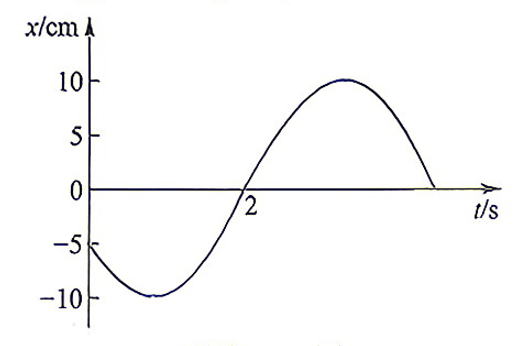
\includegraphics[width=0.3\linewidth]{figure/4-17}
	\caption{习题4-17图}
	\label{fig:4-17}
\end{figure}


\item[\textbf{4-18}]
一个质点沿 $x$ 轴做简谐振动,振幅为 $12\,\mathrm{cm}$,周期为 $2\,\mathrm{s}$.当 $t=0$ 时,位移为 $6\,\mathrm{cm}$,且向 $x$ 轴正方向运动.
\begin{enumerate}
	\item 求振动表达式；
	\item 求 $t=0.5\,\mathrm{s}$ 时,质点的位置、速度和加速度；
	\item 如果在某时刻质点位于 $x=-6\,\mathrm{cm}$,且向 $x$ 轴负方向运动,求从该位置回到平衡位置所需要的最短时间.
\end{enumerate}

\item[\textbf{4-19}]
弹簧振子沿 $x$ 轴做简谐振动.已知振动体最大位移为 $x_m=0.4\,\mathrm{m}$时最大回复力大小为 $F=0.8\,\mathrm{N}$,最大速度为 $v_m=0.8\pi\,\mathrm{m\cdot s^{-1}}$,又知 $t=0$ 的位移为 $+0.2\,\mathrm{m}$,且初速度与所选 $x$ 轴方向相反.求:
\begin{enumerate}
	\item 振动的能量；
	\item 该振动的表达式.
\end{enumerate}

\item[\textbf{4-21}]
两个同方向同频率的简谐振动曲线如习题4-21图所示.
\begin{enumerate}
	\item 求合振动的振幅；
	\item 求合振动的表达式.
\end{enumerate}

\begin{figure}[H]
	\centering
	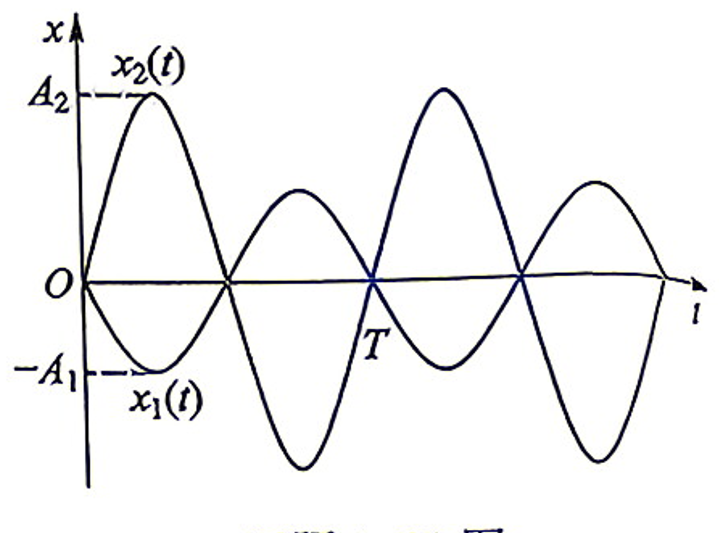
\includegraphics[width=0.3\linewidth]{figure/4-21}
	\caption{习题4-21图}
	\label{fig:4-21}
\end{figure}


\item[\textbf{4-22}]
已知一平面简谐波的波函数为$y=0.25\cos(125t-0.37x)\quad (\mathrm{SI}\ \text{单位})$分别求:
\begin{enumerate}
	\item $x_1=10\,\mathrm{m}$ 和 $x_2=25\,\mathrm{m}$ 两点处质元的振动方程；
	\item $x_1$ 和 $x_2$ 两质点间的振动相位差；
	\item $t=4\,\mathrm{s}$ 时 $x_1$ 点的振动位移.
\end{enumerate}

\item[\textbf{4-24}]
习题4-24图示为一平面简谐波在 $t=0$ 时刻的波形图,求:
\begin{enumerate}
	\item 该波的波函数；
	\item $P$ 处质元的振动方程.
\end{enumerate}

\begin{figure}[H]
	\centering
	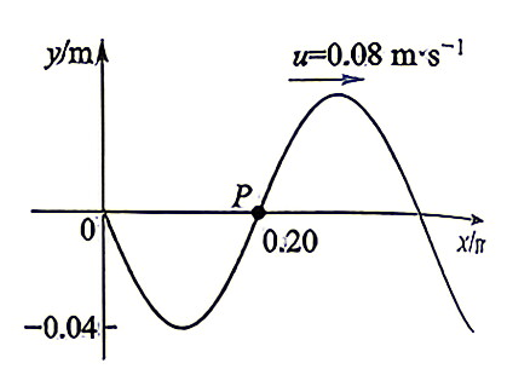
\includegraphics[width=0.3\linewidth]{figure/4-24}
	\caption{习题4-24图}
	\label{fig:4-24}
\end{figure}


\item[\textbf{4-25}]
已知一沿 $x$ 正方向传播的平面余弦波,$t=\dfrac{1}{3}\,\mathrm{s}$ 时刻的波形如习题4-25图所示,且周期 $T$ 为 $2\,\mathrm{s}$.

\begin{figure}[H]
	\centering
	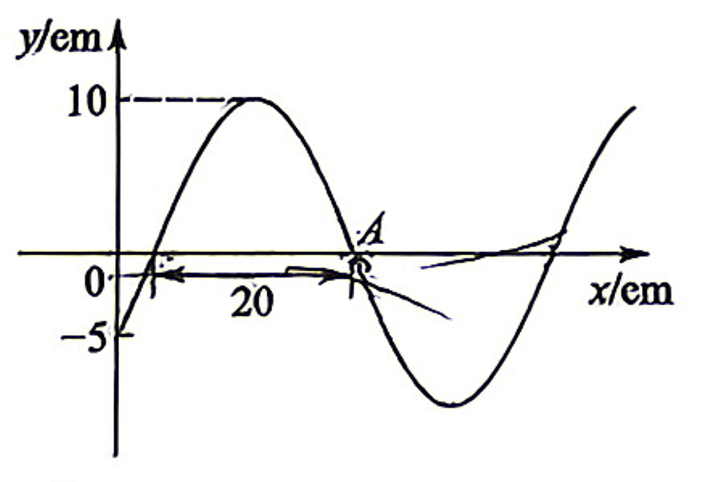
\includegraphics[width=0.3\linewidth]{figure/4-25}
	\caption{习题4-25图}
	\label{fig:4-25}
\end{figure}


\begin{enumerate}
	\item 写出 $O$ 点的振动表达式；
	\item 写出该波的波函数；
	\item 写出 $A$ 点的振动表达式；
	\item 写出 $A$ 点离 $O$ 点的距离.
\end{enumerate}

\item[\textbf{4-26}]
一平面简谐波以波速度 $u=0.8\,\mathrm{m\cdot s^{-1}}$ 沿 $x$ 轴负方向传播,已知原点的振动曲线如习题4-26图所示.试写出:
\begin{enumerate}
	\item 原点的振动表达式；
	\item 波函数；
	\item 同一时刻相距 $1\,\mathrm{m}$ 的两点之间的相位差.
\end{enumerate}

\begin{figure}[H]
	\centering
	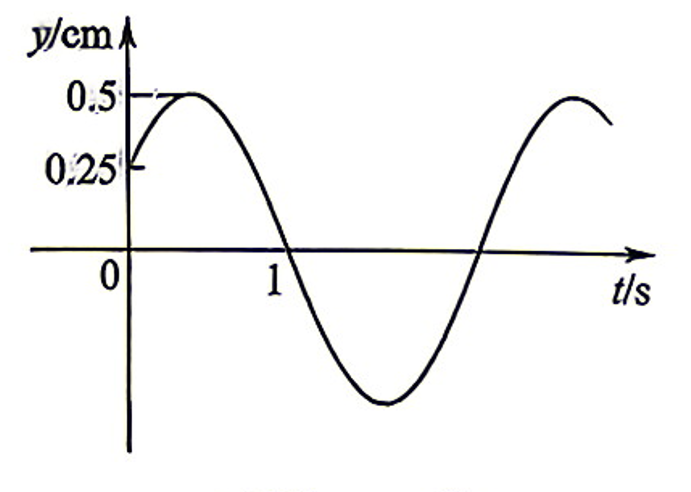
\includegraphics[width=0.3\linewidth]{figure/4-26}
	\caption{习题4-26图}
	\label{fig:4-26}
\end{figure}


\item[\textbf{4-30}]
设 $S_1$ 与 $S_2$ 为两个相干波源,相距 $\dfrac{1}{4}$ 波长,$S_1$ 比 $S_2$ 的相位超前 $\dfrac{\pi}{2}$.若两波在 $S_1$、$S_2$ 连线方向上的强度相同且不随距离变化,问 $S_1$、$S_2$ 连线上在 $S_1$ 外侧各点合成波的强度如何？在 $S_2$ 外侧各点的强度又如何？	
	
\end{enumerate}

\newpage

\subsection*{习题4题解}

\textbf{4-7题解：}
\setcounter{equation}{0}
\renewcommand{\theHequation}{4-7.\arabic{equation}}

\textbf{解答过程：}
设沿 $x$ 轴传播的平面简谐波方程为公式（\ref{eq:47-1}）：
\begin{equation}\label{eq:47-1}
	y = A \cos(\omega t - kx)
\end{equation}

介质中体积为 $\Delta V$ 的某质元的动能 $E_k$ 由速度 $v = \frac{\partial y}{\partial t}$ 决定，得到公式（\ref{eq:47-2}）：
\begin{equation}\label{eq:47-2}
	E_k = \frac{1}{2} \rho \Delta V v^2 = \frac{1}{2} \rho \Delta V A^2 \omega^2 \sin^2(\omega t - kx)
\end{equation}

该质元的弹性势能 $E_p$ 由介质的相对形变 $\frac{\partial y}{\partial x}$ 决定，得到公式（\ref{eq:47-3}）：
\begin{equation}\label{eq:47-3}
	E_p = \frac{1}{2} \rho \Delta V A^2 \omega^2 \sin^2(\omega t - kx)
\end{equation}

对比公式（\ref{eq:47-2}）与公式（\ref{eq:47-3}）可知，介质质元的动能与势能随时间的变化是完全同步的。
当质元处于平衡位置时，位移 $y=0$。由公式（\ref{eq:47-1}）推导相位关系：
\begin{align*}
	A \cos(\omega t - kx) &= 0 \\
	\implies \cos(\omega t - kx) &= 0 \\
	\implies \sin^2(\omega t - kx) &= 1
\end{align*}
将此结果代入公式（\ref{eq:47-2}）与公式（\ref{eq:47-3}），可知此时动能 $E_k$ 与势能 $E_p$ 同时达到最大值。
因此，正确选项为 \textbf{C}。

\textbf{易混淆知识点：}
本题极易将波动过程中的“开放系统质元”与机械振动中的“孤立系统振子”混淆。具体区别如下表所示：

\begin{table}[htbp]
	\centering
	\small
	\renewcommand{\arraystretch}{1.4}
	\begin{tabular}{|p{2.2cm}|p{5.5cm}|p{5.5cm}|}
		\hline
		\textbf{对比维度} & \textbf{简谐波中的介质质元} & \textbf{孤立系统的简谐振子} \\ \hline
		系统性质 & 开放系统，不断接收和传递能量 & 孤立系统，总机械能守恒 \\ \hline
		能量变化 & 同步变化（同相），同时达到极值 & 相互转化（反相），此消彼长 \\ \hline
		过平衡位置 & 形变与速度皆达最大，\textbf{动能最大，势能最大} & 速度最大、形变为零，\textbf{动能最大，势能为零} \\ \hline
		在最大位移 & 形变与速度皆为零，\textbf{动能为零，势能为零} & 速度为零、形变最大，\textbf{动能为零，势能最大} \\ \hline
	\end{tabular}
\end{table}
\textcolor{red}{注：本题若以期末复习考试为主，则主要记住表格即可，推导过程了解即可。}

\vspace{2em}

\textbf{4-11题解： }
\setcounter{equation}{0}

%\renewcommand{\theequation}{4-11.\arabic{equation}}%这句是设置标号前缀的（4-11.1...）
\renewcommand{\theHequation}{4-11.\arabic{equation}}%这句是定义超链接在4-11题内跳转的，防止乱跳。
\textbf{答案： }
$10$ ， $-\pi/2$

\textbf{解答过程： }
设两个简谐振动分别对应旋转矢量 $\vec{A}_1$ 和 $\vec{A}_2$，合振动对应矢量 $\vec{A}$。根据矢量合成法则建立公式（\ref{eq:4-11-v}）：
\begin{equation}\label{eq:4-11-v}
	\vec{A} = \vec{A}_1 + \vec{A}_2
\end{equation}
对由 $\vec{A}$、$\vec{A}_1$ 和 $\vec{A}_2$ 构成的矢量三角形应用余弦定理，得到求解第二个振动振幅 $A_2$ 的公式（\ref{eq:4-11-cos}）：
\begin{equation}\label{eq:4-11-cos}
	A_2^2 = A^2 + A_1^2 - 2AA_1\cos(\varphi - \varphi_1)
\end{equation}
将已知条件 $A = 20\text{ cm}$、$A_1 = 10\sqrt{3}\text{ cm}$ 且相位差 $\varphi - \varphi_1 = \pi/6$ 代入公式（\ref{eq:4-11-cos}）中展开：
\begin{align*}
	A_2^2 &= 20^2 + (10\sqrt{3})^2 - 2(20)(10\sqrt{3})\cos\left(\frac{\pi}{6}\right) \\
	&= 400 + 300 - 400\sqrt{3} \times \frac{\sqrt{3}}{2} \\
	&= 100
\end{align*}
解得第二个简谐振动的振幅 $A_2 = 10\text{ cm}$。

为求两者相位差，可建立平面直角坐标系，令 $\vec{A}_1$ 位于 $x$ 轴正半轴（即设 $\varphi_1 = 0$）。此时合矢量 $\vec{A}$ 的相角为 $\pi/6$，将其写为直角坐标形式：
\begin{align*}
	\vec{A} &= (20\cos 30^\circ, 20\sin 30^\circ) = (10\sqrt{3}, 10) \\
	\vec{A}_1 &= (10\sqrt{3}, 0)
\end{align*}
结合公式（\ref{eq:4-11-v}）求解 $\vec{A}_2$ 的坐标：
\begin{align*}
	\vec{A}_2 &= \vec{A} - \vec{A}_1 = (0, 10)
\end{align*}
可以看出 $\vec{A}_2$ 垂直于 $\vec{A}_1$ 沿 $y$ 轴向上，即其初相 $\varphi_2 = \pi/2$。题目要求第一、第二两个振动的相位差，如公式（\ref{eq:4-11-phase}）所示：
\begin{equation}\label{eq:4-11-phase}
	\varphi_1 - \varphi_2 = 0 - \frac{\pi}{2} = -\frac{\pi}{2}
\end{equation}
故两个空分别填 $10$ 和 $-\pi/2$。

\textbf{易混淆知识点： }
1. 使用旋转矢量法求解时，许多人习惯直接盲目套用合振幅公式 $A^2 = A_1^2 + A_2^2 + 2A_1A_2\cos(\varphi_2 - \varphi_1)$。但在本题中 $A_2$ 和两者相位差均为未知量，直接代入会形成无法直接求解的复杂方程。灵活利用矢量减法 $\vec{A}_2 = \vec{A} - \vec{A}_1$ 结合余弦定理是破题捷径。

2. 计算相位差时必须仔细审题。常规题目往往询问“第二个与第一个的相位差”（即 $\varphi_2 - \varphi_1$），而本题特别设问 $\varphi_1 - \varphi_2$，若不加注意极易漏写负号。

\vspace{2em}

\textbf{4-15题解： }
\setcounter{equation}{0}
\renewcommand{\theHequation}{4-15.\arabic{equation}}

\textbf{答案： }
$y = 0.1\cos(7\sqrt{2}t + \pi)\text{ (SI)}$

\textbf{解答过程： }
首先求解弹簧的劲度系数 $k$。当挂上物体静止时，系统处于平衡状态，弹力与重力等大反向，建立公式（\ref{eq:4-15-k}）：
\begin{equation}\label{eq:4-15-k}
	mg = k\Delta l
\end{equation}
已知弹簧原长 $l_0 = 0.5\text{ m}$，平衡长度 $l = 0.6\text{ m}$，则静伸长量 $\Delta l = l - l_0 = 0.1\text{ m}$，代入数据得：
\begin{align*}
	k &= \frac{0.1 \times 9.8}{0.1} = 9.8\text{ N/m}
\end{align*}
弹簧振子系统的固有角频率 $\omega$ 由公式（\ref{eq:4-15-w}）计算：
\begin{equation}\label{eq:4-15-w}
	\omega = \sqrt{\frac{k}{m}} = \sqrt{\frac{9.8}{0.1}} = \sqrt{98} = 7\sqrt{2}\text{ rad/s}
\end{equation}
设该简谐振动的位移学方程为公式（\ref{eq:4-15-y}）：
\begin{equation}\label{eq:4-15-y}
	y = A\cos(\omega t + \varphi_0)
\end{equation}
依题意取竖直向下为坐标系的正方向，并以受力平衡位置（即弹簧长度为 $0.6\text{ m}$ 处）为坐标原点 $y=0$。
将物体上推至弹簧缩回到原长处放手，即 $t=0$ 时：
\begin{align*}
	y_0 &= 0.5 - 0.6 = -0.1\text{ m} \\
	v_0 &= 0\text{ m/s}
\end{align*}
利用初始条件求解振动方程的振幅 $A$ 和初相 $\varphi_0$：
\begin{align*}
	A &= \sqrt{y_0^2 + \left(\frac{v_0}{\omega}\right)^2} = \sqrt{(-0.1)^2 + 0} = 0.1\text{ m} \\
	y_0 &= A\cos\varphi_0 \implies \cos\varphi_0 = \frac{-0.1}{0.1} = -1 \implies \varphi_0 = \pi
\end{align*}
将求得的各项参数代回公式（\ref{eq:4-15-y}），写出最终的振动表达式：
\begin{align*}
	y &= 0.1\cos(7\sqrt{2}t + \pi)\text{ (SI)}
\end{align*}

\textbf{易混淆知识点： }
1. \textbf{平衡位置的绝对基准}：弹簧振子的简谐运动必须围绕“受力平衡点”而非“弹簧原长点”展开。在列出振动方程时，坐标 $y$ 必须且只能表示物体偏离此受力平衡位置的位移大小和方向。

2. \textbf{坐标正方向对初相的决定性影响}：题目明确规定“取竖直向下为正方向”，这意味着将物体上推回到原长（即向上移动）所对应的初始坐标是负值（$y_0 = -0.1\text{ m}$）。如果不严格遵守题目给定的正方向将其记作正值，将会导致求出的初相为 $0$，使最终得出的振动方程在相位上发生完全反转。

\vspace{2em}

\textbf{4-17题解： }
\setcounter{equation}{0}
\renewcommand{\theHequation}{4-17.\arabic{equation}}

\textbf{答案： }
$x = 10 \cos\left(\frac{5\pi}{12} t + \frac{2\pi}{3}\right) \text{ (cm)}$

\textbf{解答过程： }
设简谐振动的运动学方程为公式（\ref{eq:4-17-x}）：
\begin{equation}\label{eq:4-17-x}
	x = A \cos(\omega t + \phi_0)
\end{equation}
对位移求导，可得振动速度方程为公式（\ref{eq:4-17-v}）：
\begin{equation}\label{eq:4-17-v}
	v = \frac{dx}{dt} = -A\omega \sin(\omega t + \phi_0)
\end{equation}
由图中振动曲线可知，振幅 $A = 10 \text{ cm}$。
当 $t = 0$ 时，初始位移 $x_0 = -5 \text{ cm}$，代入公式（\ref{eq:4-17-x}）得：
\begin{align*}
	10 \cos\phi_0 &= -5 \\
	\implies \cos\phi_0 &= -\frac{1}{2}
\end{align*}
同时，在 $t=0$ 处曲线的斜率为负，说明此时速度 $v_0 < 0$。代入公式（\ref{eq:4-17-v}）可知 $\sin\phi_0 > 0$。综合可得初相 $\phi_0 = \frac{2\pi}{3}$。
由图可知，当 $t = 2 \text{ s}$ 时，质点首次经过平衡位置且向正方向运动（斜率为正），即 $x = 0$ 且 $v > 0$。结合公式（\ref{eq:4-17-x}）和（\ref{eq:4-17-v}）有：
\begin{align*}
	10 \cos\left(2\omega + \frac{2\pi}{3}\right) &= 0 \\
	-10\omega \sin\left(2\omega + \frac{2\pi}{3}\right) &> 0
\end{align*}
要满足余弦为0且正弦为负，该时刻的相位应为 $\frac{3\pi}{2}$，建立相位等式为公式（\ref{eq:4-17-phase}）：
\begin{equation}\label{eq:4-17-phase}
	2\omega + \frac{2\pi}{3} = \frac{3\pi}{2}
\end{equation}
解公式（\ref{eq:4-17-phase}）得到角频率 $\omega = \frac{5\pi}{12} \text{ rad/s}$。
将 $A$、$\omega$、$\phi_0$ 代回公式（\ref{eq:4-17-x}），得到最终振动方程：
\begin{align*}
	x &= 10 \cos\left(\frac{5\pi}{12} t + \frac{2\pi}{3}\right) \text{ (cm)}
\end{align*}

\textbf{易混淆知识点： }
本题极易在通过 $t=2\text{ s}$ 点求解 $\omega$ 时出错。很多学生会错误地认为从 $t=0$ 到 $t=2$ 是四分之一个周期或直接代入 $\cos=0$ 的任意解（如 $\pi/2$）。必须结合图像斜率（速度方向）来判定 $t=2\text{ s}$ 时刻对应的确切相位是 $3\pi/2$ 而非 $\pi/2$。

\vspace{2em}

\textbf{4-18题解： }
\setcounter{equation}{0}
\renewcommand{\theHequation}{4-18.\arabic{equation}}

\textbf{答案： }
(1) $x = 12 \cos\left(\pi t - \frac{\pi}{3}\right) \text{ (cm)}$
(2) 位置 $6\sqrt{3} \text{ cm}$，速度 $-6\pi \text{ cm/s}$，加速度 $-6\sqrt{3}\pi^2 \text{ cm/s}^2$
(3) $\frac{5}{6} \text{ s}$

\textbf{解答过程： }
(1) 已知周期 $T = 2 \text{ s}$，由周期与角频率关系建立公式（\ref{eq:4-18-omega}）：
\begin{equation}\label{eq:4-18-omega}
	\omega = \frac{2\pi}{T} = \frac{2\pi}{2} = \pi \text{ rad/s}
\end{equation}
设振动方程为 $x = A \cos(\omega t + \phi_0)$。已知振幅 $A = 12 \text{ cm}$。
当 $t = 0$ 时，位移 $x_0 = 6 \text{ cm}$ 且向 $x$ 轴正向运动（$v_0 > 0$），代入公式建立条件方程组（\ref{eq:4-18-init}）：
\begin{equation}\label{eq:4-18-init}
	\begin{cases}
		12 \cos\phi_0 = 6 \\
		-12\pi \sin\phi_0 > 0
	\end{cases}
\end{equation}
由公式（\ref{eq:4-18-init}）解得 $\cos\phi_0 = \frac{1}{2}$ 且 $\sin\phi_0 < 0$，故初相 $\phi_0 = -\frac{\pi}{3}$。
得到振动表达式为：
\begin{align*}
	x &= 12 \cos\left(\pi t - \frac{\pi}{3}\right) \text{ (cm)}
\end{align*}

(2) 质点的速度和加速度方程分别对位移求一阶和二阶导数，得到公式（\ref{eq:4-18-v}）和公式（\ref{eq:4-18-a}）：
\begin{equation}\label{eq:4-18-v}
	v = \frac{dx}{dt} = -12\pi \sin\left(\pi t - \frac{\pi}{3}\right)
\end{equation}
\begin{equation}\label{eq:4-18-a}
	a = \frac{dv}{dt} = -12\pi^2 \cos\left(\pi t - \frac{\pi}{3}\right)
\end{equation}
将 $t = 0.5 \text{ s}$ 代入位移、速度和加速度方程中：
\begin{align*}
	x &= 12 \cos\left(0.5\pi - \frac{\pi}{3}\right) = 12 \cos\left(\frac{\pi}{6}\right) = 6\sqrt{3} \text{ cm} \\
	v &= -12\pi \sin\left(0.5\pi - \frac{\pi}{3}\right) = -12\pi \sin\left(\frac{\pi}{6}\right) = -6\pi \text{ cm/s} \\
	a &= -12\pi^2 \cos\left(0.5\pi - \frac{\pi}{3}\right) = -12\pi^2 \cos\left(\frac{\pi}{6}\right) = -6\sqrt{3}\pi^2 \text{ cm/s}^2
\end{align*}

(3) 设某时刻位移 $x = -6 \text{ cm}$ 且向负方向运动，设此时相位为 $\Phi$。建立方程（\ref{eq:4-18-target1}）：
\begin{equation}\label{eq:4-18-target1}
	12 \cos\Phi = -6 \implies \cos\Phi = -\frac{1}{2}
\end{equation}
由于向负方向运动，即速度 $v < 0$，得出 $\sin\Phi > 0$。满足条件的相位 $\Phi = \frac{2\pi}{3}$。
质点回到平衡位置即 $x = 0$，下一个平衡位置对应相位为 $\Phi' = \frac{3\pi}{2}$。
相位差 $\Delta\Phi$ 计算如公式（\ref{eq:4-18-dphi}）所示：
\begin{equation}\label{eq:4-18-dphi}
	\Delta\Phi = \frac{3\pi}{2} - \frac{2\pi}{3} = \frac{5\pi}{6}
\end{equation}
所需最短时间 $\Delta t$ 由公式（\ref{eq:4-18-dt}）给出：
\begin{equation}\label{eq:4-18-dt}
	\Delta t = \frac{\Delta\Phi}{\omega} = \frac{\frac{5\pi}{6}}{\pi} = \frac{5}{6} \text{ s}
\end{equation}

\textbf{易混淆知识点： }
第(3)问求解最短时间时，必须准确判定初始状态与目标状态的“绝对相位”。已知 $x=-6$ 且 $v<0$，说明质点正在第二象限的旋转矢量上（$\Phi=2\pi/3$），向着负向最大位移（$\Phi=\pi$）进发。回到平衡位置指的是越过负向最大点后折返至 $x=0$ 的位置（对应旋转矢量转至 $\Phi=3\pi/2$）。\textcolor{red}{切勿将目标点错当成 $\pi/2$ 而得出负的时间值。}

\textbf{本人对于第（3）问的感悟：}：对于第4章的题目，最重要也是最有助于理解的东西就是：旋转圆法，旋转圆都是从逆时针出发的（不管振动方向正向还是反向），因为旋转圆表示的是时间，时间是不可逆的。下面将详细讲解一下关于旋转圆的知识点（主要以本题第（3）问为主）：
\section*{物理思维工具：“参考圆”（旋转矢量法）}

要把这一段完全搞懂，我们需要借助一个强大的物理思维工具：\textbf{“参考圆”（也叫旋转矢量法）}。

很多同学搞不懂“相位”，是因为只盯着直线上来回跑的质点看。如果我们把这段直线运动，想象成是一个圆周运动在直线上的投影，一切就豁然开朗了。为了让你彻底弄懂，我们一步步来“走”完这个过程。

\subsection*{第一步：理解“相位”到底是什么？}

想象有一个圆，半径就是振幅 $A = 12\text{ cm}$。圆上有一个点（我们叫它“参考点”），正在逆时针做匀速圆周运动。
这个参考点在横轴（$x$ 轴）上的影子，就是我们在题目中研究的那个做简谐振动的质点。

\textbf{参考点转过的角度，就是所谓的“相位”。}

在圆上：
\begin{itemize}
	\item 最右边（3点钟方向）是 $0$ 度 ($0$)。
	\item 最上面（12点钟方向）是 $90$ 度 ($\pi/2$)。
	\item 最左边（9点钟方向）是 $180$ 度 ($\pi$)。
	\item 最下面（6点钟方向）是 $270$ 度 ($3\pi/2$)。
\end{itemize}

\subsection*{第二步：代入题目的三个关键状态}

现在我们让圆上的点开始逆时针转，盯着它在 $x$ 轴上的影子（质点）看：

\textbf{状态 1：当前所在位置（相位 $2\pi/3$）}
\begin{itemize}
	\item \textbf{圆上的位置：} 点转到了第二象限，角度是 $120^\circ$（即 $2\pi/3$）。
	\item \textbf{影子的状态（质点）：} 此时影子在 $x$ 轴负半轴的 $-6\text{ cm}$ 处。因为圆上的点正在往左上角转，所以它的影子也正在向左（负方向）运动。这就对应了题目说的“位于 $x = -6\text{ cm}$，且向 $x$ 轴负方向运动”。
\end{itemize}

\textbf{状态 2：走到负最大位移处（相位 $\pi$）}
\begin{itemize}
	\item \textbf{圆上的位置：} 点继续逆时针转，到达了最左边，也就是 9 点钟方向。这个位置的角度是 $180^\circ$（即 $\pi$）。
	\item \textbf{影子的状态（质点）：} 此时影子到达了 $x$ 轴的最左端，也就是 $x = -12\text{ cm}$ 的位置。此时影子不能再往左了，它的速度瞬间减为 $0$，准备掉头向右走。
\end{itemize}

\textbf{状态 3：掉头回到平衡位置（相位 $3\pi/2$）}
\begin{itemize}
	\item \textbf{圆上的位置：} 点从最左边继续逆时针转，来到了最底部，也就是 6 点钟方向。这个位置的角度是 $270^\circ$（即 $3\pi/2$）。
	\item \textbf{影子的状态（质点）：} 此时影子刚好走到了 $x$ 轴的正中间（原点 $x = 0$），也就是平衡位置。因为圆上的点正在向右下角转，所以它的影子此时正在向右（正方向）运动。
\end{itemize}

\subsection*{总结一下区别：}

\begin{itemize}
	\item 当相位是 $\pi/2$（最上面）时，质点在平衡位置 $x=0$，但正在\textbf{向左走}。
	\item 当相位是 $3\pi/2$（最下面）时，质点在平衡位置 $x=0$，但正在\textbf{向右走}。
\end{itemize}

因为质点是从左边 ($-6\text{ cm}$) 掉头往右走回来的，所以它经过平衡位置时必然是向右走的，因此对应的相位只能是底部的 $3\pi/2$。

\vspace{2em}

\textbf{4-19题解： }
\setcounter{equation}{0}
\renewcommand{\theHequation}{4-19.\arabic{equation}}

\textbf{答案： }
(1) $0.16 \text{ J}$
(2) $x = 0.4 \cos\left(2\pi t + \frac{\pi}{3}\right) \text{ (SI)}$

\textbf{解答过程： }
(1) 根据简谐振动的动力学特征，最大回复力 $F_m$ 与振幅 $A$（即最大位移 $x_m$）的关系建立公式（\ref{eq:4-19-k}）：
\begin{equation}\label{eq:4-19-k}
	F_m = k A
\end{equation}
代入已知数据 $F_m = 0.8 \text{ N}$ 和 $A = x_m = 0.4 \text{ m}$，解得系统的等效劲度系数 $k$：
\begin{align*}
	k &= \frac{0.8}{0.4} = 2 \text{ N/m}
\end{align*}
\textcolor{red}{因为是简谐振动，所以振动系统的总能量 $E$ 等于系统经过最大位移时的最大弹性势能}，由公式（\ref{eq:4-19-e}）计算得出：
\begin{equation}\label{eq:4-19-e}
	E = \frac{1}{2} k A^2
\end{equation}
代入数据得：
\begin{align*}
	E &= \frac{1}{2} \times 2 \times 0.4^2 = 0.16 \text{ J}
\end{align*}

(2) 设简谐振动的运动学表达式为 $x = A \cos(\omega t + \phi_0)$。
已知最大速度 $v_m = 0.8\pi \text{ m/s}$，利用最大速度与角频率的关系建立公式（\ref{eq:4-19-w}）：
\begin{equation}\label{eq:4-19-w}
	v_m = \omega A
\end{equation}
代入求得角频率 $\omega$：
\begin{align*}
	\omega &= \frac{0.8\pi}{0.4} = 2\pi \text{ rad/s}
\end{align*}
当 $t=0$ 时，初始位移 $x_0 = +0.2 \text{ m}$，将其代入振动方程：
\begin{align*}
	0.4 \cos\phi_0 &= 0.2 \implies \cos\phi_0 = \frac{1}{2}
\end{align*}
同时已知初速度与 $x$ 轴正向相反（即 $v_0 < 0$），而速度方程 $v = -A\omega \sin(\omega t + \phi_0)$，故要求 $t=0$ 时 $\sin\phi_0 > 0$。综合正弦与余弦的条件得出初相 $\phi_0 = \frac{\pi}{3}$。
综上，该振动的最终表达式为：
\begin{align*}
	x &= 0.4 \cos\left(2\pi t + \frac{\pi}{3}\right) \text{ (SI)}
\end{align*}

\textbf{易混淆知识点： }
在求解简谐振动能量时，很多学生习惯于寻找振子质量 $m$ 并利用 $E = \frac{1}{2}mv_m^2$ 来计算。但本题并未直接给出质量。灵活理解简谐运动的本质，利用“最大回复力”求出劲度系数 $k$，直接通过最大势能公式 $E = \frac{1}{2}kA^2$ 求解，是突破此类“隐去质量”题目的关键途径。

\vspace{2em}

\textbf{4-21题解： }
\setcounter{equation}{0}
\renewcommand{\theHequation}{4-21.\arabic{equation}}

\textbf{答案： }
(1) $\sqrt{A_1^2 + A_2^2}$
(2) $x = \sqrt{A_1^2 + A_2^2} \cos\left(\frac{2\pi}{T} t - \pi + \arctan\frac{A_2}{A_1}\right)$

\textbf{解答过程： }
(1) 根据振动曲线图，我们首先写出两个分振动的独立表达式。
$x_1(t)$ 曲线在 $t=0$ 时恰好位于负向最大位移处，其振幅为 $A_1$，周期为 $T$。设角频率为 $\omega = \frac{2\pi}{T}$，则其初相 $\phi_1 = \pi$（或$-\pi$），振动方程写为公式（\ref{eq:4-21-x1}）：
\begin{equation}\label{eq:4-21-x1}
	x_1 = A_1 \cos(\omega t + \pi)
\end{equation}
$x_2(t)$ 曲线在 $t=0$ 时刚好通过平衡位置且斜率为正（向正向运动），其振幅为 $A_2$，初相 $\phi_2 = -\frac{\pi}{2}$，振动方程写为公式（\ref{eq:4-21-x2}）：
\begin{equation}\label{eq:4-21-x2}
	x_2 = A_2 \cos\left(\omega t - \frac{\pi}{2}\right)
\end{equation}
两个振动的相位差 $\Delta \phi = \phi_2 - \phi_1 = -\frac{\pi}{2} - \pi = -\frac{3\pi}{2}$（等效于 $\frac{\pi}{2}$ 的相位差），这说明两个振动在相位上是相互正交的。
利用矢量合成法则，合振幅 $A$ 的计算如公式（\ref{eq:4-21-A}）所示：
\begin{equation}\label{eq:4-21-A}
	A = \sqrt{A_1^2 + A_2^2 + 2A_1 A_2 \cos\left(\frac{\pi}{2}\right)} = \sqrt{A_1^2 + A_2^2}
\end{equation}

(2) 设合振动的表达式为 $x = A \cos(\omega t + \phi)$。我们可以利用直角坐标系投影法来求解合初相 $\phi$：
在相量图中，将 $x_1$ 和 $x_2$ 的旋转矢量在 $x$ 轴和 $y$ 轴上分解，建立 $t=0$ 时刻的分量方程组（\ref{eq:4-21-proj}）：
\begin{equation}\label{eq:4-21-proj}
	\begin{cases}
		A \cos\phi = A_1 \cos\pi + A_2 \cos\left(-\frac{\pi}{2}\right) = -A_1 \\
		A \sin\phi = A_1 \sin\pi + A_2 \sin\left(-\frac{\pi}{2}\right) = -A_2
	\end{cases}
\end{equation}
由方程组（\ref{eq:4-21-proj}）可知，合相量的余弦分量和正弦分量均为负值，这明确界定了合相量 $\phi$ 必然位于第三象限。
利用正切关系求解角度：
\begin{align*}
	\tan\phi &= \frac{-A_2}{-A_1} = \frac{A_2}{A_1} \\
	\implies \phi &= -\pi + \arctan\frac{A_2}{A_1}
\end{align*}
代入图示给出的时间周期参数 $\omega = \frac{2\pi}{T}$，得到最终完整的合振动表达式：
\begin{align*}
	x &= \sqrt{A_1^2 + A_2^2} \cos\left(\frac{2\pi}{T} t - \pi + \arctan\frac{A_2}{A_1}\right)
\end{align*}

\textbf{易混淆知识点： }
在合成两个同频简谐振动求解合初相 $\phi$ 时，极易直接套用公式 $\tan\phi = \frac{A_2}{A_1}$ 然后按计算器得出 $\phi = \arctan(A_2/A_1)$，从而误将初相定在第一象限。必须严格根据旋转矢量的横轴投影（本题为 $-A_1$）和纵轴投影（本题为 $-A_2$）的具体符号来判定其所在的象限。由于本题两投影皆为负，合相量必定在第三象限，因此在求得反正切主值后必须加上（或减去）$\pi$ 以进行象限修正。

\textbf{补充：}
根据\ref{eq:4-21-x1}和\ref{eq:4-21-x2}可得出初相位分别为$\pi$(x负半轴)，和$-\frac{\pi}{2}$(y负半轴)，可以做出矢量合成图：

% TODO: \usepackage{graphicx} required
\begin{figure}[H]
	\centering
	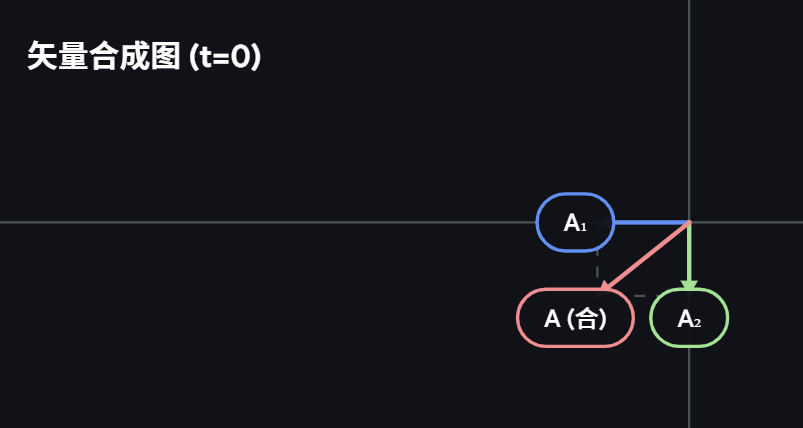
\includegraphics[width=0.4\linewidth]{figure/slt}
	\caption{辅助矢量图}
	\label{fig:slt}
\end{figure}

\textcolor{red}{再次说明：根据初相位做矢量图和旋转圆法在第4章非常重要，一定要重点掌握！}

\vspace{2em}

\textbf{4-22题解： }
\setcounter{equation}{0}
\renewcommand{\theHequation}{4-22.\arabic{equation}}

\textbf{答案： }
(1) $x_1=10\,\text{m}$ 处质元的振动方程为 $y_1 = 0.25 \cos(125t - 3.7)$ (SI)；$x_2=25\,\text{m}$ 处质元的振动方程为 $y_2 = 0.25 \cos(125t - 9.25)$ (SI)。\\
(2) $x_1$ 和 $x_2$ 两质点间的振动相位差为 $\Delta \phi = 5.55\,\text{rad}$。\\
(3) $t=4\,\text{s}$ 时 $x_1$ 点的振动位移为 $y \approx 0.249\,\text{m}$。

\textbf{解答过程： }
已知平面简谐波的波函数为：
\begin{equation}\label{eq:4-22-1}
	y(x,t) = 0.25 \cos(125t - 0.37x)
\end{equation}

(1) 求解某坐标点的振动方程，即将该点的位置坐标 $x$ 代入波函数即可：
对于 $x_1 = 10\,\text{m}$ 的质元，代入公式(\ref{eq:4-22-1})得其振动方程为：
\begin{align*}
	y_1 &= 0.25 \cos(125t - 0.37 \times 10) \\
	&= 0.25 \cos(125t - 3.7) \quad (\text{SI})
\end{align*}

对于 $x_2 = 25\,\text{m}$ 的质元，代入公式(\ref{eq:4-22-1})得其振动方程为：
\begin{align*}
	y_2 &= 0.25 \cos(125t - 0.37 \times 25) \\
	&= 0.25 \cos(125t - 9.25) \quad (\text{SI})
\end{align*}

(2) 平面简谐波中，同波线上两质点间的相位差 $\Delta \phi$ 由波矢 $k$ 与空间距离 $\Delta x$ 决定。由给定的波函数可知波数 $k = 0.37\,\text{rad/m}$，相位差公式为：
\begin{equation}\label{eq:4-22-2}
	\Delta \phi = k |x_2 - x_1|
\end{equation}
将数据代入公式(\ref{eq:4-22-2})可得：
\begin{align*}
	\Delta \phi &= 0.37 \times |25 - 10| \\
	&= 0.37 \times 15 \\
	&= 5.55\,\text{rad}
\end{align*}

(3) 求特定时间、特定位置的振动位移，需将 $t=4\,\text{s}$ 与 $x_1=10\,\text{m}$ 代入波函数(\ref{eq:4-22-1})中：
\begin{align*}
	y &= 0.25 \cos(125 \times 4 - 0.37 \times 10) \\
	&= 0.25 \cos(500 - 3.7) \\
	&= 0.25 \cos(496.3)
\end{align*}
计算可知 $496.3\,\text{rad} \approx 79 \times 2\pi - 0.0716\,\text{rad}$，因此：
\begin{align*}
	y &\approx 0.25 \times \cos(-0.0716) \\
	&\approx 0.25 \times 0.9974 \\
	&\approx 0.249\,\text{m}
\end{align*}

\textbf{易混淆知识点： }
1. \textbf{波函数与振动方程的区别}：波函数 $y(x,t)$ 描述了介质中所有质点在任意时刻的位移（包含空间变量 $x$ 和时间变量 $t$）；而振动方程 $y(t)$ 描述的是某一特定质元（给定确定的 $x$ 值）单纯随时间的变化规律。

2. \textbf{相位差的计算}：同一时刻波线上两点的相位差公式为 $\Delta \phi = k\Delta x = \frac{2\pi}{\lambda}\Delta x$。注意不要与同一质点在不同时刻的相位差 $\Delta \phi = \omega\Delta t$ 混淆。

3. \textbf{计算器弧度制设置}：在计算第(3)问中的 $\cos(496.3)$ 时，括号内的数值单位为“弧度”（rad），而非“角度”（degree）。在进行具体数值计算时，务必确保科学计算器处于弧度制（Rad）模式，否则会导致位移结果完全错误。

\textcolor{red}{注意：公式(\ref{eq:4-22-2})属于易忘公式，一定要牢记！！！}

\vspace{2em}

\textbf{4-24题解： }
\setcounter{equation}{0}
\renewcommand{\theHequation}{4-24.\arabic{equation}}

\textbf{答案： }
(1) 该波的波函数为 $y = 0.04 \cos(0.4\pi t - 5\pi x - \frac{\pi}{2})$ (SI)。\\
(2) $P$ 处质元的振动方程为 $y_P = 0.04 \cos(0.4\pi t + \frac{\pi}{2})$ (SI)。

\textbf{解答过程： }
从波形图可知，该简谐波的振幅 $A = 0.04\,\text{m}$。
波在 $t=0$ 时刻由原点 $O$ 传播至 $P$ 点（从位移为0向下振动到再次位移为0）经历半个波形，故半波长 $\frac{\lambda}{2} = 0.20\,\text{m}$，解得波长 $\lambda = 0.40\,\text{m}$。
由波速 $u = 0.08\,\text{m/s}$，可得周期 $T$ 为：
\begin{align*}
	T = \frac{\lambda}{u} = \frac{0.40}{0.08} = 5\,\text{s}
\end{align*}
进而求得角频率 $\omega$ 和波数 $k$ 分别为：
\begin{align*}
	\omega &= \frac{2\pi}{T} = 0.4\pi\,\text{rad/s} \\
	k &= \frac{2\pi}{\lambda} = 5\pi\,\text{rad/m}
\end{align*}
设平面简谐波的波函数一般形式为：
\begin{equation}\label{eq:4-24-1}
	y(x,t) = A \cos(\omega t - kx + \phi_0)
\end{equation}
考察原点 $x=0$ 处的质元，在 $t=0$ 时刻位移 $y=0$。结合波沿 $x$ 轴正向传播，可知原点处质元此刻正受到其左侧波峰的带动，向 $y$ 轴正方向运动（即速度 $v > 0$）。
代入初始条件：
\begin{align*}
	y(0,0) &= A \cos\phi_0 = 0 \\
	v(0,0) &= -A\omega \sin\phi_0 > 0
\end{align*}
由以上两式解得初相位 $\phi_0 = -\frac{\pi}{2}$。
将各参数代入公式(\ref{eq:4-24-1})，得到该波的波函数为：
\begin{equation}\label{eq:4-24-2}
	y = 0.04 \cos(0.4\pi t - 5\pi x - \frac{\pi}{2}) \quad (\text{SI})
\end{equation}

(2) 求解 $P$ 处质元的振动方程，从图中可知 $P$ 点的坐标为 $x = 0.20\,\text{m}$。
将其代入已求得的波函数公式(\ref{eq:4-24-2})中：
\begin{align*}
	y_P &= 0.04 \cos(0.4\pi t - 5\pi \times 0.20 - \frac{\pi}{2}) \\
	&= 0.04 \cos(0.4\pi t - \pi - \frac{\pi}{2}) \\
	&= 0.04 \cos(0.4\pi t - \frac{3\pi}{2})
\end{align*}
利用三角函数诱导公式 $\cos(\alpha - \frac{3\pi}{2}) = \cos(\alpha + \frac{\pi}{2})$，化简可得 $P$ 处质元的振动方程：
\begin{equation}\label{eq:4-24-3}
	y_P = 0.04 \cos(0.4\pi t + \frac{\pi}{2}) \quad (\text{SI})
\end{equation}

\textbf{易混淆知识点： }
1. \textbf{初相位符号的判定}：已知 $y=0$ 只能得出初相为 $\pm\pi/2$，此时必须结合波的传播方向利用\textcolor{red}{“同侧法”或“微商法”(本人推荐用同侧法)}判断质点振动速度方向。本题波向右传，原点即将迎来波峰，故向上振动（速度为正），从而确定初相为 $-\pi/2$ 而不是 $+\pi/2$。

2. \textbf{波形空间距离与波长的关系}：图中 $P$ 点位于 $x=0.20\,\text{m}$ 处，由于波形正好是一个完整的下半波谷，因此这段距离对应的是 $\lambda/2$，切勿看成 $1/4$ 波长或一整个波长。

3. \textbf{主值区间的化简}：在求解质点振动方程得到相位差 $-3\pi/2$ 后，建议利用诱导公式将其转化到 $(-\pi, \pi]$ 的主值区间内（即 $+\pi/2$）。虽然两者在数学上等价，但在物理学中，使用主值区间表达相位更为规范和直观。

\vspace{2em}

\textbf{4-25题解： }
\setcounter{equation}{0}
\renewcommand{\theHequation}{4-25.\arabic{equation}}

\textbf{答案： }
(1) $O$ 点的振动表达式为 $y_O = 0.1 \cos(\pi t + \frac{\pi}{3})$ (SI)。\\
(2) 该波的波函数为 $y = 0.1 \cos(\pi t - 5\pi x + \frac{\pi}{3})$ (SI)。\\
(3) $A$ 点的振动表达式为 $y_A = 0.1 \cos(\pi t - \frac{5\pi}{6})$ (SI)。\\
(4) $A$ 点离 $O$ 点的距离为 $\frac{7}{30}\,\text{m}$ （或 $\approx 0.233\,\text{m}$ / $\frac{70}{3}\,\text{cm}$）。

\textbf{解答过程： }
已知周期 $T = 2\,\text{s}$，则角频率为：
\begin{align*}
	\omega = \frac{2\pi}{T} = \pi\,\text{rad/s}
\end{align*}
设沿 $x$ 轴正方向传播的平面简谐波的波函数一般形式为：
\begin{equation}\label{eq:4-25-1}
	y(x,t) = A \cos(\omega t - kx + \phi_0)
\end{equation}
由波形图可知，振幅 $A = 10\,\text{cm} = 0.1\,\text{m}$。
观察放大后的波形图细节，标注为 $20\,\text{cm}$ 的箭头起始于第一个过平衡位置向上的点（波节），终止于点 $A$（下一个过平衡位置向下的波节）。两个相邻且振动方向相反的波节之间的距离正好为半个波长，因此：
\begin{align*}
	\frac{\lambda}{2} &= 20\,\text{cm} = 0.2\,\text{m} \\
	\lambda &= 0.4\,\text{m}
\end{align*}
据此求得波数 $k$ 为：
\begin{equation}\label{eq:4-25-2}
	k = \frac{2\pi}{\lambda} = \frac{2\pi}{0.4} = 5\pi\,\text{rad/m}
\end{equation}
在 $t = \frac{1}{3}\,\text{s}$ 时刻，原点 $O$ ($x=0$) 的位移 $y = -5\,\text{cm} = -0.05\,\text{m}$，且根据波形图，该点处波形曲线的斜率 $\frac{\partial y}{\partial x} > 0$。
将 $x=0, t=\frac{1}{3}\,\text{s}$ 代入波函数：
\begin{align*}
	y(0, \frac{1}{3}) &= 0.1 \cos(\frac{\pi}{3} + \phi_0) = -0.05 \\
	\cos(\frac{\pi}{3} + \phi_0) &= -0.5
\end{align*}
对波函数求空间偏导数 $\frac{\partial y}{\partial x} = Ak \sin(\omega t - kx + \phi_0)$，代入 $O$ 点状态可知 $\sin(\frac{\pi}{3} + \phi_0) > 0$，故相位主值应取第二象限角，即 $\frac{\pi}{3} + \phi_0 = \frac{2\pi}{3}$。由此解得初相位：
\begin{equation}\label{eq:4-25-3}
	\phi_0 = \frac{\pi}{3}
\end{equation}

(1) 求解 $O$ 点的振动表达式，将 $x=0, \omega=\pi, \phi_0=\frac{\pi}{3}$ 代入一般形式：
\begin{equation}\label{eq:4-25-4}
	y_O = 0.1 \cos(\pi t + \frac{\pi}{3}) \quad (\text{SI})
\end{equation}

(2) 将求得的各参数代入，得到该波的波函数为：
\begin{equation}\label{eq:4-25-5}
	y(x,t) = 0.1 \cos(\pi t - 5\pi x + \frac{\pi}{3})\quad (\text{SI})
\end{equation}

(3) 在 $t = \frac{1}{3}\,\text{s}$ 的波形图上，$A$ 点位于波峰右侧的第一个平衡位置（向下穿过 $x$ 轴）。
将 $t = \frac{1}{3}\,\text{s}$ 代入波函数，该时刻的波形方程相角分布为 $(\frac{2\pi}{3} - 5\pi x)$。
已知波峰处相角为 $0$，其右侧紧邻的过零点 $A$ 点的相角应为 $-\frac{\pi}{2}$。令：
\begin{align*}
	\frac{2\pi}{3} - 5\pi x_A &= -\frac{\pi}{2} \\
	5\pi x_A &= \frac{7\pi}{6}
\end{align*}
解得 $A$ 点的坐标 $x_A = \frac{7}{30}\,\text{m}$。
将 $x_A$ 代入波函数求解 $A$ 点的振动表达式：
\begin{align*}
	y_A &= 0.1 \cos(\pi t - 5\pi \times \frac{7}{30} + \frac{\pi}{3}) \\
	&= 0.1 \cos(\pi t - \frac{7\pi}{6} + \frac{2\pi}{6})
\end{align*}
化简可得：
\begin{equation}\label{eq:4-25-6}
	y_A = 0.1 \cos(\pi t - \frac{5\pi}{6}) \quad (\text{SI})
\end{equation}

% 由(3)中求得的 $A$ 点坐标可知，$A$ 点离原点 $O$ 的距离即为 $x_A$ 的绝对值：
%\begin{align*}
%	\Delta x = x_A - 0 = \frac{7}{30}\,\text{m}
%\end{align*}
(4)由第(1)问可知$\mathbf{O}$点的振动方程(见(公式\ref{eq:4-25-4}))，可知$\mathbf{O}$点的初相位是$\frac{\pi}{3}$.
由第(3)问可知$\mathbf{A}$点的振动方程(见(公式\ref{eq:4-25-6})),可知$\mathbf{A}$点的初相位是$-\frac{5\pi}{6}$.

所以有：$x_1=\frac{\pi}{3}$,$x_2=-\frac{5\pi}{6}$,$k=5\pi$

由相位差公式：
\begin{equation}\label{eq:4-25-7}
	\Delta x = \frac{\Delta \phi}{k}\,\text{cm}
\end{equation}

带入公式得：
\begin{align*}
	\Delta x = \frac{70}{3}\,\text{cm} \approx 23.33\,\text{cm}
\end{align*}
(换算为米即为 $\frac{7}{30}\,\text{m}$)

\textbf{易混淆知识点： }
1. \textbf{波形图中尺寸标注的识别}：极易将图中平行于 $x$ 轴的长度标注误认为某特征点（如波峰）的绝对横坐标。本题中的“20”带有双向箭头，其物理意义是图示两个“过零点（波节）”之间的相对距离。由于这两个过零点斜率一正一负，它们之间恰好跨越了半个波长（$\lambda/2$）。

2. \textbf{空间相位与振动相位的关系}：在确定 $A$ 点坐标时，需利用空间相位的滞后性。波沿 $+x$ 传播，$A$ 位于波峰前方（更靠近 $+x$ 方向），因此其接受到该波峰状态的时间更晚，在同一时刻的波形图上，其相位比波峰落后 $\frac{\pi}{2}$（即相角为 $-\frac{\pi}{2}$）。

3. \textbf{角频率与波数的量纲统一}：在波函数中若 $x$ 使用米（m）作单位，$k$ 必须是 $\text{rad/m}$；若 $x$ 使用厘米（cm），$k$ 需为 $\text{rad/cm}$。最终写成标准 SI 单位时，所有长度相关的量（振幅 $A$、坐标 $x$、波数 $k$）都必须统一到米制系统下。

\vspace{2em}

\textbf{4-26题解： }
\setcounter{equation}{0}
\renewcommand{\theHequation}{4-26.\arabic{equation}}

\textbf{答案： }
(1) 原点的振动表达式为 $y_O = 0.005 \cos(\frac{5\pi}{6}t - \frac{\pi}{3})$ (SI)。\\
(2) 该波的波函数为 $y = 0.005 \cos(\frac{5\pi}{6}t + \frac{25\pi}{24}x - \frac{\pi}{3})$ (SI)。\\
(3) 同一时刻相距 $1\,\text{m}$ 的两点之间的相位差为 $\Delta \phi = \frac{25\pi}{24}\,\text{rad}$。

\textbf{解答过程： }
(1) 由原点 $O$ 的振动曲线（$y-t$ 图）可知，振幅 $A = 0.5\,\text{cm} = 0.005\,\text{m}$。
设原点的振动表达式一般形式为：
\begin{equation}\label{eq:4-26-1}
	y_O(t) = A \cos(\omega t + \phi_0)
\end{equation}
在 $t = 0$ 时刻，位移 $y(0) = 0.25\,\text{cm} = \frac{1}{2}A$。代入振动表达式：
\begin{align*}
	A \cos\phi_0 = \frac{1}{2}A \implies \cos\phi_0 = 0.5
\end{align*}
且由图可知 $t=0$ 时刻曲线正在上升阶段（向 $+y$ 方向运动），即此时速度 $v(0) = -A\omega\sin\phi_0 > 0$，所以 $\sin\phi_0 < 0$。因此可确定初相位：
\begin{align*}
	\phi_0 = -\frac{\pi}{3}
\end{align*}
观察图形，在 $t = 1\,\text{s}$ 时刻，质点第一次回到平衡位置且曲线向下（向 $-y$ 方向运动），此时振动相位应为 $\frac{\pi}{2}$：
\begin{align*}
	\omega \times 1 - \frac{\pi}{3} = \frac{\pi}{2} \implies \omega = \frac{5\pi}{6}\,\text{rad/s}
\end{align*}
将 $A, \omega, \phi_0$ 代入公式(\ref{eq:4-26-1})，得到原点 $O$ 的振动表达式为：
\begin{align*}
	y_O = 0.005 \cos(\frac{5\pi}{6}t - \frac{\pi}{3}) \quad (\text{SI})
\end{align*}

(2) 已知平面简谐波沿 $x$ 轴负方向传播，波速 $u = 0.8\,\text{m/s}$。波沿负方向传播的波函数一般形式为（空间相位项为 $+kx$）：
\begin{equation}\label{eq:4-26-2}
	y(x,t) = A \cos(\omega t + kx + \phi_0)
\end{equation}
利用波速求波数 $k$：
\begin{align*}
	k = \frac{\omega}{u} = \frac{5\pi/6}{0.8} = \frac{5\pi/6}{4/5} = \frac{25\pi}{24}\,\text{rad/m}
\end{align*}
将各参数代入公式(\ref{eq:4-26-2})，得到该平面简谐波的波函数为：
\begin{align*}
	y = 0.005 \cos(\frac{5\pi}{6}t + \frac{25\pi}{24}x - \frac{\pi}{3}) \quad (\text{SI})
\end{align*}

(3) 在同一时刻 $t$，波线上相距 $\Delta x$ 的两质点间的振动相位差由空间相位公式决定：
\begin{equation}\label{eq:4-26-3}
	\Delta \phi = k \Delta x
\end{equation}
已知两点相距 $\Delta x = 1\,\text{m}$，代入公式(\ref{eq:4-26-3})得：
\begin{align*}
	\Delta \phi = \frac{25\pi}{24} \times 1 = \frac{25\pi}{24}\,\text{rad}
\end{align*}

\textbf{易混淆知识点： }
1. \textbf{振动图与波形图的区分}：本题给出的是原点的“振动曲线”（横坐标为时间 $t$），描述的是单一质点随时间的位移变化。切不可将其误认为是“波形图”（横坐标为空间 $x$）去直接读波长或判断波的传播方向。

2. \textbf{传播方向与空间相位符号}：当波沿 $x$ 轴正方向传播时，波函数中的空间项为 $-kx$（前方质点相位滞后）；而本题明确指出波“沿 $x$ 轴负方向传播”，因此空间项必须为 $+kx$。

3. \textbf{由平衡点推断角频率}：在利用 $t=1\,\text{s}$ 时的过零点求角频率 $\omega$ 时，需注意该质点是“由正向负”穿过平衡位置（斜率为负），对应的振动相位为 $\pi/2$（而非 $3\pi/2$ 或 $-\pi/2$）。结合 $t=0$ 的初相位 $-\pi/3$，这段时间内的相位变化量为 $\Delta\phi = \pi/2 - (-\pi/3) = 5\pi/6$，从而直接求出 $\omega$。

\vspace{2em}

\textbf{4-30题解： }
\setcounter{equation}{0}
\renewcommand{\theHequation}{4-30.\arabic{equation}}

\textbf{答案： }
设单波的强度为 $I_0$。在 $S_1$ 外侧各点合成波的强度为 $0$；在 $S_2$ 外侧各点合成波的强度为 $4I_0$。

\textbf{解答过程： }
设两相干波源 $S_1$、$S_2$ 在空间某点 $P$ 引起的波的初相分别为 $\phi_{10}$ 和 $\phi_{20}$。由题意知，$S_1$ 比 $S_2$ 相位超前 $\frac{\pi}{2}$，即初相位差为：
\begin{align*}
	\Delta \phi_0 = \phi_{10} - \phi_{20} = \frac{\pi}{2}
\end{align*}
设空间中某考察点 $P$ 到两波源的距离分别为 $r_1$ 和 $r_2$，则两波在 $P$ 点的绝对相位差 $\Delta \phi$ 为：
\begin{equation}\label{eq:4-30-1}
	\Delta \phi = \phi_1 - \phi_2 = (\phi_{10} - \frac{2\pi}{\lambda} r_1) - (\phi_{20} - \frac{2\pi}{\lambda} r_2) = \Delta \phi_0 - \frac{2\pi}{\lambda} (r_1 - r_2)
\end{equation}
两波在空间任一点的合成波强度公式为：
\begin{equation}\label{eq:4-30-2}
	I = I_1 + I_2 + 2\sqrt{I_1 I_2} \cos(\Delta \phi)
\end{equation}
已知沿连线方向强度相同且不随距离变化，设 $I_1 = I_2 = I_0$。

(1) 对于位于 $S_1$ 外侧的各点（即在 $S_1, S_2$ 连线上且位于 $S_1$ 左侧），由于两波源相距 $d = \frac{\lambda}{4}$，该区域各点到两波源的波程差恒为：
\begin{align*}
	r_1 - r_2 = -d = -\frac{\lambda}{4}
\end{align*}
将其代入相位差公式(\ref{eq:4-30-1})可得：
\begin{align*}
	\Delta \phi &= \frac{\pi}{2} - \frac{2\pi}{\lambda} \times (-\frac{\lambda}{4}) \\
	&= \frac{\pi}{2} + \frac{\pi}{2} = \pi
\end{align*}
将 $\Delta \phi = \pi$ 代入合成强度公式(\ref{eq:4-30-2})，得到 $S_1$ 外侧各点的强度：
\begin{align*}
	I_{S_1外} &= I_0 + I_0 + 2I_0 \cos\pi \\
	&= 2I_0 - 2I_0 = 0
\end{align*}
即合成波强度为 $0$（发生完全相消干涉）。

(2) 对于位于 $S_2$ 外侧的各点（即在 $S_1, S_2$ 连线上且位于 $S_2$ 右侧），该区域各点到两波源的波程差恒为：
\begin{align*}
	r_1 - r_2 = d = \frac{\lambda}{4}
\end{align*}
同样将其代入相位差公式(\ref{eq:4-30-1})可得：
\begin{align*}
	\Delta \phi &= \frac{\pi}{2} - \frac{2\pi}{\lambda} \times (\frac{\lambda}{4}) \\
	&= \frac{\pi}{2} - \frac{\pi}{2} = 0
\end{align*}
将 $\Delta \phi = 0$ 代入合成强度公式(\ref{eq:4-30-2})，得到 $S_2$ 外侧各点的强度：
\begin{align*}
	I_{S_2外} &= I_0 + I_0 + 2I_0 \cos 0 \\
	&= 2I_0 + 2I_0 = 4I_0
\end{align*}
即合成波强度为 $4I_0$（发生完全相长干涉）。

\textbf{易混淆知识点： }
1. \textbf{相位差公式中符号的严格对应}：在计算 $\Delta \phi = \phi_1 - \phi_2$ 时，波程差项必须严格对应为 $- \frac{2\pi}{\lambda}(r_1 - r_2)$。如果将其颠倒写成 $(r_2 - r_1)$ 且未改变前面的负号，会导致波程差带来的相位符号完全反转，从而得出 $S_1$ 与 $S_2$ 外侧强度互换的错误结论。

2. \textbf{连线外侧波程差的恒定性}：在两个波源连线的延长线上（即“外侧”），空间任意一点到两个波源的距离之差 $|r_1 - r_2|$ 始终恒等于两波源的物理间距 $d$。这也是为什么题目中提及该直线上外侧各点强度“不随距离变化”的几何原因。

\newpage

\subsection{习题7}

\subsubsection*{本人建议：}
在做习题七之前，应该先去完成第七章的例题，\textcolor{red}{习题中有很多结论直接出自例题的答案。}

\begin{enumerate}
	\item [\textbf{7-9}]
	一个细玻璃棒被弯成半径为$\mathbf{R}$的半圆形，沿其上半部分均匀分布有电荷$\mathbf{+Q}$,沿其下半部分均匀分布有电荷$\mathbf{-Q}$,如习题7-9图所示。试求圆心$\mathbf{O}$处的电场强度。
	% TODO: \usepackage{graphicx} required
	\begin{figure}[H]
		\centering
		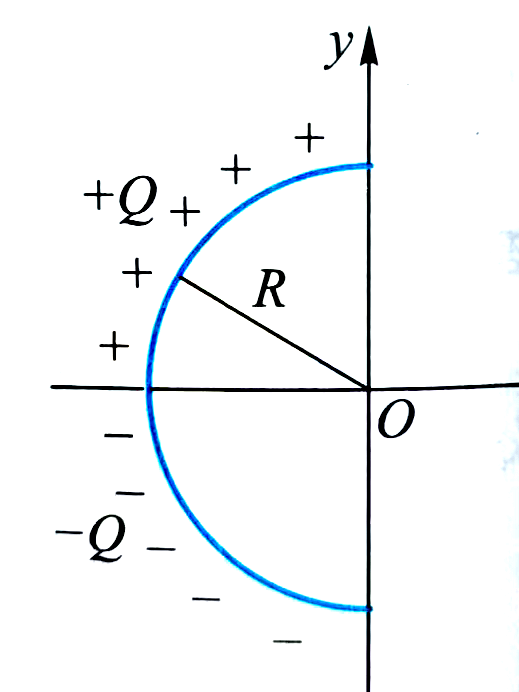
\includegraphics[width=0.2\linewidth]{figure/7-9}
		\caption{图7-9}
		\label{fig:7-9}
	\end{figure}
	
	\item [\textbf{7-11}]
	如习题7-11图所示两个无限大的平行平面都均匀带电，电荷的面密度分别为$\sigma_1$和$\sigma_2$，试求空间各处场强。
	% TODO: \usepackage{graphicx} required
	\begin{figure}[H]
		\centering
		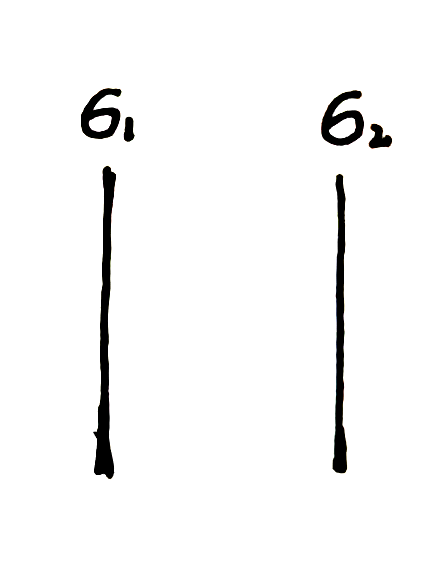
\includegraphics[width=0.2\linewidth]{figure/7-11}
		\caption{图7-11}
		\label{fig:7-11}
	\end{figure}
	
	\item [\textbf{7-13}]
	如习题7-13图所示，在点电荷$q$的电厂中,选取以$q$为中心、$\mathbf{R}$为半径的球面上一点$\mathbf{P}$作为电势零点,求与点电荷$q$距离为$r$的$\mathbf{P^\prime}$点的电势。
	% TODO: \usepackage{graphicx} required
	\begin{figure}[H]
		\centering
		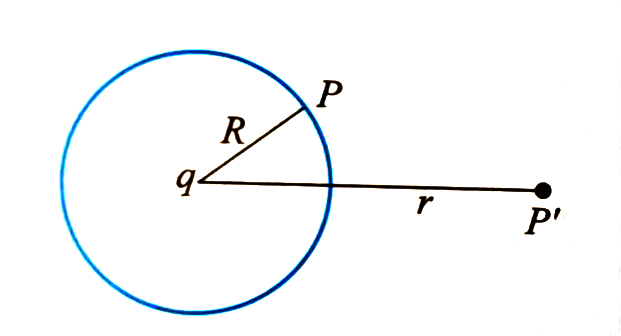
\includegraphics[width=0.3\linewidth]{figure/7-13}
		\caption{图7-13}
		\label{fig:7-13}
	\end{figure}
	
	\item [\textbf{7-14}]
	如习题7-14图所示,边长为$a$的等边三角形的三个顶点上，分别放置着三个正的点电荷$q$、$2q$、$3q$.若将另一个正点电荷$\mathbf{Q}$从无穷远处移到三角形的中心$\mathbf{O}$处，外力所做的功多大?
	% TODO: \usepackage{graphicx} required
	\begin{figure}[H]
		\centering
		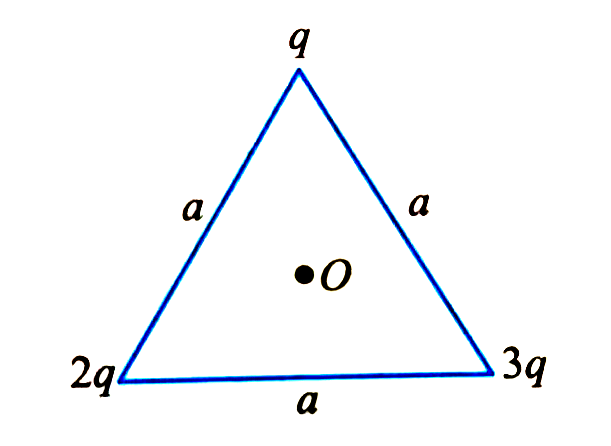
\includegraphics[width=0.3\linewidth]{figure/7-14}
		\caption{图7-14}
		\label{fig:7-14}
	\end{figure}
	
	\item [\textbf{7-15}]
	如习题7-15图所示，试验电荷$q$在点电荷$\mathbf{+Q}$产生的电场中，沿半径为$\mathbf{R}$的整个圆弧的$3/4$圆弧轨道，由$a$点移动到$d$点的过程中电场力做的功为多少？从$d$点移动到无限远处的过程中，电场力做的功为多少？
	
	% TODO: \usepackage{graphicx} required
	\begin{figure}[H]
		\centering
		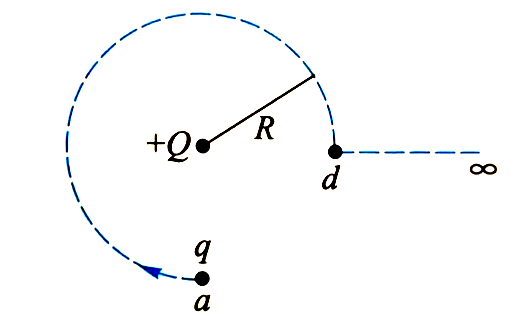
\includegraphics[width=0.3\linewidth]{figure/7-15}
		\caption{图7-15}
		\label{fig:7-15}
	\end{figure}
	
	\item [\textbf{7-17}]
	电荷$q$均匀分布在长为$2l$的细杆上，求在杆外延长线上与杆端距离为$a$的$P$点的电势(设无限远处为电势零点)
	
\end{enumerate}

\newpage

\subsection*{习题7题解}

\textbf{7-9题解： }
\setcounter{equation}{0}
\renewcommand{\theHequation}{7-9.\arabic{equation}}

\textbf{答案： }
圆心 $O$ 处的电场强度大小为 $E = \frac{Q}{\pi^2 \varepsilon_0 R^2}$，方向沿 $y$ 轴负方向。矢量形式为 $\mathbf{E} = -\frac{Q}{\pi^2\varepsilon_0 R^2} \mathbf{j}$。

\textbf{解答过程： }
这道题需要通过微元法（取电荷元 $dq$）并结合对称性来进行积分求解。

\textbf{1. 分析对称性与建立坐标系}
如图所示，半圆弧位于 $y$ 轴左侧。上半部分带正电 $+Q$，下半部分带负电 $-Q$。

\begin{itemize}
	\item 对于上半圆弧上的任意一个微小电荷元 $+dq$，它在圆心 $O$ 处产生的电场 $d\mathbf{E}_+$ 指向第四象限。
	\item 在下半圆弧对称位置上，会存在一个电荷元 $-dq$，它在圆心 $O$ 处产生的电场 $d\mathbf{E}_-$ 指向第三象限。
	\item 分解这两个电场：\textbf{它们的水平分量（$x$ 轴方向）大小相等、方向相反，完美相互抵消；而它们的竖直分量（$y$ 轴方向）都沿着负 $y$ 轴方向，会相互叠加。}
	\item 因此，圆心 $O$ 处的总电场方向\textbf{必定是竖直向下}（沿负 $y$ 轴方向）。
\end{itemize}

\textbf{2. 求解上半圆弧产生的电场}
首先求出线电荷密度 $\lambda$。上半圆弧的长度是 $L = \frac{1}{2}\pi R$，所以它的线电荷密度为：
\begin{equation}\label{eq:7-9-1}
	\lambda = \frac{Q}{\frac{\pi R}{2}} = \frac{2Q}{\pi R}
\end{equation}
我们设定一个角 $\theta$（从负 $x$ 轴向上偏转的角度，$\theta \in [0, \pi/2]$）。在这个位置取一段微小弧长 $dl = R d\theta$，它所带的微小电荷量为：
\begin{equation}\label{eq:7-9-2}
	dq = \lambda dl = \frac{2Q}{\pi R} R d\theta = \frac{2Q}{\pi} d\theta
\end{equation}
这个点电荷 $dq$ 在圆心 $O$ 处产生的电场大小为：
\begin{align*}
	dE = \frac{1}{4\pi\varepsilon_0} \frac{dq}{R^2}
\end{align*}
我们只关心它在竖直方向（$y$ 轴）的分量 $dE_y$。根据几何关系，这个分量的大小为：
\begin{equation}\label{eq:7-9-3}
	dE_y = dE \sin\theta = \frac{1}{4\pi\varepsilon_0 R^2} \left( \frac{2Q}{\pi} d\theta \right) \sin\theta
\end{equation}
对整个上半圆弧（$\theta$ 从 $0$ 到 $\pi/2$）进行积分：
\begin{align*}
	E_{y1} &= \int_{0}^{\pi/2} \frac{2Q}{4\pi^2\varepsilon_0 R^2} \sin\theta d\theta \\
	&= \frac{Q}{2\pi^2\varepsilon_0 R^2} \int_{0}^{\pi/2} \sin\theta d\theta \\
	&= \frac{Q}{2\pi^2\varepsilon_0 R^2} [-\cos\theta]_0^{\pi/2} \\
	&= \frac{Q}{2\pi^2\varepsilon_0 R^2} (0 - (-1)) = \frac{Q}{2\pi^2\varepsilon_0 R^2}
\end{align*}
方向竖直向下。

\textbf{3. 叠加求总场强}
根据我们第一步的对称性分析，下半圆弧（带负电 $-Q$）在圆心 $O$ 处产生的竖直向下的电场，其大小与上半圆弧完全相同。
因此，总电场大小为：
\begin{equation}\label{eq:7-9-4}
	E = 2 \times E_{y1} = 2 \times \frac{Q}{2\pi^2\varepsilon_0 R^2} = \frac{Q}{\pi^2\varepsilon_0 R^2}
\end{equation}
最终答案：圆心 $O$ 处的电场强度大小为 $\frac{Q}{\pi^2\varepsilon_0 R^2}$，方向沿 $y$ 轴负向。写成矢量形式为：
\begin{equation}\label{eq:7-9-5}
	\mathbf{E} = -\frac{Q}{\pi^2\varepsilon_0 R^2} \mathbf{j}
\end{equation}

\textbf{易混淆知识点： }
1. \textbf{积分变量与坐标系的巧妙定义}：图解方法中将角度 $\theta$ 定义为“从负 $x$ 轴向上偏转的角度”，且积分区间设定为 $[0, \pi/2]$。这种处理方式比直接使用标准极坐标系（从正 $x$ 轴起算，区间为 $[\pi/2, \pi]$）更加简便直观，但在进行这种自定义时，必须确保投影关系（如这里的 $dE_y = dE \sin\theta$）与你的定义严密吻合。

2. \textbf{线电荷密度的分母极易算错}：\textbf{在计算 $\lambda$ 时，由于带电部分分别只占据了整个圆周的“四分之一”（上半弧和下半弧各自的长度为 $\frac{\pi R}{2}$），}\textcolor{red}{故分母必须是 $\frac{\pi R}{2}$，从而得到 $\lambda = \frac{2Q}{\pi R}$。}许多人在做题时会本能地将其除以半圆周长 $\pi R$，从而遗漏了分子上的 $2$。

\vspace{2em}

\textbf{7-11题解： }
\setcounter{equation}{0}
\renewcommand{\theHequation}{7-11.\arabic{equation}}

\textbf{答案： }
设水平向右为正方向（单位矢量 $\vec{n}$）。\\
两平面左侧区域场强：$\vec{E}_I = -\frac{\sigma_1 + \sigma_2}{2\varepsilon_0}\vec{n}$；\\
两平面之间区域场强：$\vec{E}_{II} = \frac{\sigma_1 - \sigma_2}{2\varepsilon_0}\vec{n}$；\\
两平面右侧区域场强：$\vec{E}_{III} = \frac{\sigma_1 + \sigma_2}{2\varepsilon_0}\vec{n}$。

\textbf{解答过程： }
\textcolor{red}{根据无限大均匀带电平面的高斯定理推导结果，}\textbf{表面}电荷密度为 $\sigma$ 的无限大平面在周围空间产生的电场是匀强电场，其场强大小为：
\begin{equation}\label{eq:7-11-1}
	E = \frac{\sigma}{2\varepsilon_0}
\end{equation}

(\textcolor{red}{注：}该公式在L7-8处，课本\textbf{P172}页)

\textbf{方向垂直于带电平面。若 $\sigma > 0$，场强指向远离平面的方向；若 $\sigma < 0$，场强指向平面的方向。}

设平行平面所在位置的法线方向\textcolor{red}{（水平向右）}为正向单位矢量 $\vec{n}$。
左侧平面（电荷密度 $\sigma_1$）在空间产生的匀强电场分布为：
位于平面左侧时：$\vec{E}_{1L} = -\frac{\sigma_1}{2\varepsilon_0}\vec{n}$
位于平面右侧时：$\vec{E}_{1R} = \frac{\sigma_1}{2\varepsilon_0}\vec{n}$

右侧平面（电荷密度 $\sigma_2$）在空间产生的匀强电场分布为：
位于平面左侧时：$\vec{E}_{2L} = -\frac{\sigma_2}{2\varepsilon_0}\vec{n}$
位于平面右侧时：$\vec{E}_{2R} = \frac{\sigma_2}{2\varepsilon_0}\vec{n}$

\textbf{根据电场强度的叠加原理，空间任一点的总场强等于两平面在该点单独产生场强的矢量和：}
\begin{equation}\label{eq:7-11-2}
	\vec{E} = \vec{E}_1 + \vec{E}_2
\end{equation}

整个空间被两平面分为三个区域进行讨论：
(1) 在第一平面左侧区域（区域 I）：该区域位于两平面的左侧，两者电场均向左。
\begin{align*}
	\vec{E}_I = \vec{E}_{1L} + \vec{E}_{2L} = -\frac{\sigma_1}{2\varepsilon_0}\vec{n} - \frac{\sigma_2}{2\varepsilon_0}\vec{n} = -\frac{\sigma_1 + \sigma_2}{2\varepsilon_0}\vec{n}
\end{align*}

(2) 在两平面之间区域（区域 II）：该区域位于第一平面右侧、第二平面左侧。
\begin{align*}
	\vec{E}_{II} = \vec{E}_{1R} + \vec{E}_{2L} = \frac{\sigma_1}{2\varepsilon_0}\vec{n} - \frac{\sigma_2}{2\varepsilon_0}\vec{n} = \frac{\sigma_1 - \sigma_2}{2\varepsilon_0}\vec{n}
\end{align*}

(3) 在第二平面右侧区域（区域 III）：该区域位于两平面的右侧，两者电场均向右。
\begin{align*}
	\vec{E}_{III} = \vec{E}_{1R} + \vec{E}_{2R} = \frac{\sigma_1}{2\varepsilon_0}\vec{n} + \frac{\sigma_2}{2\varepsilon_0}\vec{n} = \frac{\sigma_1 + \sigma_2}{2\varepsilon_0}\vec{n}
\end{align*}

\textbf{易混淆知识点： }
1. \textbf{无限大带电平面的场强特点}：由公式(\ref{eq:7-11-1})可知，场强大小 $\frac{\sigma}{2\varepsilon_0}$ 是一个与距离完全无关的常量。在计算叠加时，无论空间点离平面有多远，只要在平面的同一侧，该平面贡献的电场大小就不会衰减。

2. \textbf{代数表达式的普适性}：在推导时，默认先假设 $\sigma_1, \sigma_2 > 0$ 并在坐标轴上定出矢量正负。最终得出的三个区域的代数表达式实际上具有绝对的通用性：如果实际情况中某平面带有负电（如电容器极板），直接将 $\sigma$ 连同负号代入相应的表达式中即可自然获得正确的方向，无需重新画图判断。

\vspace{2em}

\textbf{7-13题解： }
\setcounter{equation}{0}
\renewcommand{\theHequation}{7-13.\arabic{equation}}

\textbf{答案： }
与点电荷 $q$ 距离为 $r$ 的 $P'$ 点的电势为 $V_{P'} = \frac{q}{4\pi\varepsilon_0} \left( \frac{1}{r} - \frac{1}{R} \right)$。

\textbf{解答过程： }
\textbf{方法一：电势定义积分法（微积分法）}
根据静电场中电势的定义，空间某点 $P'$ 的电势等于把单位正电荷从该点移到电势零参考点 $P$ 的过程中电场力所作的功。
设点电荷 $q$ 到考察点的径向距离为 $x$，则点电荷在距离为 $x$ 处产生的电场强度大小为：
\begin{equation}\label{eq:7-13-1}
	E = \frac{q}{4\pi\varepsilon_0 x^2}
\end{equation}
方向沿径向。从待求点 $P'$（径向距离为 $r$）沿径向积分到电势零点 $P$（径向距离为 $R$），两点间的电势差定义为：
\begin{align*}
	V_{P'} - V_P &= \int_{P'}^{P} \vec{E} \cdot \mathrm{d}\vec{l} = \int_{r}^{R} \frac{q}{4\pi\varepsilon_0 x^2} \mathrm{d}x
\end{align*}
题意已知点 $P$ 被选作电势零点，即 $V_P = 0$。代入上式进行定积分计算：
\begin{equation}\label{eq:7-13-2}
	V_{P'} - 0 = \frac{q}{4\pi\varepsilon_0} \left[ -\frac{1}{x} \right]_{r}^{R}
\end{equation}
代入上下限，化简得到：
\begin{align*}
	V_{P'} = \frac{q}{4\pi\varepsilon_0} \left( -\frac{1}{R} - \left(-\frac{1}{r}\right) \right) = \frac{q}{4\pi\varepsilon_0} \left( \frac{1}{r} - \frac{1}{R} \right)
\end{align*}

\textbf{方法二：电势差不变法（相对电势法）}
\textcolor{red}{电场中任意两点之间的电势差是绝对的，与电势零点的选择无关。}
通常情况下，我们默认无穷远处为电势零点。此时，距离点电荷 $q$ 为 $r$ 处的电势公式为：$V = \frac{q}{4\pi\varepsilon_0 r}$。
若设无穷远处为标准零点，那么：
$P$ 点（距离为 $R$）的“绝对电势”为：
\begin{equation}\label{eq:7-13-3}
	V_P = \frac{q}{4\pi\varepsilon_0 R}
\end{equation}
$P'$ 点（距离为 $r$）的“绝对电势”为：
\begin{equation}\label{eq:7-13-4}
	V_{P'} = \frac{q}{4\pi\varepsilon_0 r}
\end{equation}
两点之间的电势差为：
\begin{align*}
	U_{P'P} = V_{P'} - V_P = \frac{q}{4\pi\varepsilon_0 r} - \frac{q}{4\pi\varepsilon_0 R} = \frac{q}{4\pi\varepsilon_0} \left( \frac{1}{r} - \frac{1}{R} \right)
\end{align*}
题目现在规定 $P$ 点为新的电势零点，即令 $V_P^{new} = 0$。\textbf{根据电势差不变的原则}，新的 $P'$ 点电势 $V_{P'}^{new}$ 必须满足：
\begin{align*}
	V_{P'}^{new} - V_P^{new} = U_{P'P}
\end{align*}
代入已知量：
\begin{equation}\label{eq:7-13-5}
	V_{P'}^{new} - 0 = \frac{q}{4\pi\varepsilon_0} \left( \frac{1}{r} - \frac{1}{R} \right)
\end{equation}
从而得到 $V_{P'}^{new} = \frac{q}{4\pi\varepsilon_0} \left( \frac{1}{r} - \frac{1}{R} \right)$。

\textbf{法一与法二的对比：}
 \textbf{方法一（积分法）}是从静电场最根本的物理定义（电场力做功）出发，普适性极强。无论电场分布多么复杂，只要能写出场强表达式，就能通过设定上下限直接积出结果。缺点是计算过程相对繁琐，高度依赖微积分基础，容易在积分上下限或正负号上出错。
 
 \textbf{方法二（电势差不变法）}是一种非常巧妙的代数替换技巧。它利用了\textbf{“电势差是绝对的”}这一物理核心性质，\textbf{通过引入已知的标准结论（以无穷远为零点的点电势公式），直接避开了复杂的微积分运算。}优点是计算简便、思路清晰，不易出现符号错误；缺点是它依赖于你已经熟记了该电荷分布在标准零点下的电势公式。

\textbf{易混淆知识点： }
1. \textbf{电势零点的相对性与电势差的绝对性}：电势的零点是可以人为任意选取的，\textbf{随着零点的改变，空间各点的电势绝对数值都会加上或减去同一个常数（发生整体平移）。}\textcolor{red}{但是，任意两点之间的“高度差”（即电势差）就像山峰之间的相对高度一样，是绝对不变的。}这也是方法二能够成立的核心物理依据。

2. \textbf{电势定义式中积分上下限的顺序}：在方法一中使用积分法 $\int_A^B \vec{E} \cdot \mathrm{d}\vec{l}$ 计算某点电势时，\textcolor{red}{积分的起点（下限）必须是待求点 $P'$（即 $x=r$），积分的终点（上限）必须是规定的电势零点 $P$（即 $x=R$）。}如果将上下限写反，会导致求出的电势带有多余的负号。

\vspace{2em}

\textbf{7-15题解： }
\setcounter{equation}{0}
\renewcommand{\theHequation}{7-15.\arabic{equation}}

\textbf{答案： }
(1) 试验电荷 $q$ 由 $a$ 点移动到 $d$ 点的过程中，电场力做的功为 $0$。\\
(2) 从 $d$ 点移动到无限远处的过程中，电场力做的功为 $W_{d\infty} = \frac{qQ}{4\pi\varepsilon_0 R}$。

\textbf{解答过程： }
(1) 静电场是保守力场，电场力做功只与电荷的初、末位置有关，而与电荷移动的具体路径无关。电场力做功的公式可以表示为：
\begin{equation}\label{eq:7-15-1}
	W_{AB} = q(V_A - V_B)
\end{equation}
在点电荷 $+Q$ 产生的电场中，距离其为 $r$ 处的电势公式为：
\begin{equation}\label{eq:7-15-2}
	V = \frac{Q}{4\pi\varepsilon_0 r}
\end{equation}
由图可知，\textbf{$a$ 点和 $d$ 点均位于以 $+Q$ 为圆心、半径为 $R$ 的圆弧上。因此，这两点处于同一个等势面上，它们的电势相等：}
\begin{align*}
	V_a = V_d = \frac{Q}{4\pi\varepsilon_0 R}
\end{align*}
根据公式(\ref{eq:7-15-1})，试验电荷 $q$ 从 $a$ 移动到 $d$ 电场力做功为：
\begin{align*}
	W_{ad} = q(V_a - V_d) = 0
\end{align*}

(2) 规定无限远处的电势为零，即 $V_\infty = 0$。
试验电荷 $q$ 从 $d$ 点移动到无限远处，电场力做功为：
\begin{align*}
	W_{d\infty} &= q(V_d - V_\infty) \\
	&= q\left(\frac{Q}{4\pi\varepsilon_0 R} - 0\right) \\
	&= \frac{qQ}{4\pi\varepsilon_0 R}
\end{align*}

\textbf{易混淆知识点： }
1. \textbf{保守力做功与路径无关}：题目特意强调了“沿整个圆弧的 3/4 圆弧轨道”移动，这是一个极具迷惑性的条件。如果不理解静电场的保守性，极易顺着题干的暗示去尝试通过力与路径的线积分 $\int \vec{F} \cdot \mathrm{d}\vec{l}$ 去计算做功，这不仅计算极其复杂（涉及到力的方向时刻改变），还容易算错。\textcolor{red}{牢记：在静电场中求做功，永远优先考虑电势差 $W=qU$。}

2. \textbf{电势的符号代入}：\textcolor{red}{在使用 $W_{AB} = q(V_A - V_B)$ 时，所有的电量（包括场源电荷 $Q$ 和试验电荷 $q$）都需要严格带入正负号。}本题虽然都是正号，但\textbf{在遇到带负电的粒子时，必须连同符号一起代入计算，否则会导致做正功还是负功的判断完全相反。}

\subsection*{7-14和7-15算功时的差异来源}
7-14 和 7-15 的公式之所以一个是“末减初”，一个是“初减末”，根本原因在于题目问的\textbf{“做功主体”}不同：
\begin{itemize}
	\item 7-14 问的是：\textbf{“外力”}做功
	\item 7-15 问的是：\textbf{“电场力”}做功
\end{itemize}

这两个力做功的物理意义和计算符号是刚好相反的。我们来详细拆解一下：

\textbf{1. 电场力做功（对应 7-15） $\rightarrow$ 必须是“初减末”}

电场力是一种保守力（和重力一样）。在物理学中，保守力做功的定义是：\textbf{保守力做功等于系统势能的减少量}。

你可以想象一个正电荷在电场中顺着电场线“顺流而下”，电场力在推着它走。此时电场力做正功，电荷的电势能就会变小（就像石头从高处掉下来，重力做正功，重力势能减少）。

因为是“减少量”，所以公式是：
$$W_{\text{电场力}} = E_{p(\text{初})} - E_{p(\text{末})} = qV_{\text{初}} - qV_{\text{末}} = q(V_{\text{初}} - V_{\text{末}})$$

\textbf{结论}：\textcolor{red}{求电场力做功，一律用初态的能量（电势）减去末态的能量（电势）。}

\textbf{2. 外力做功（对应 7-14） $\rightarrow$ 必须是“末减初”}

题目中说“将电荷从无穷远处移到中心 $O$ 处”，在大学物理中，这隐含着一个条件：\textbf{缓慢移动}（也就是动能不发生改变，始终为零）。

既然动能不增加，根据动能定理，总功必须为零。这意味着外力做的功，必须刚好抵消电场力做的功：
$$W_{\text{外力}} + W_{\text{电场力}} = 0 \implies W_{\text{外力}} = - W_{\text{电场力}}$$

外力做功的作用是什么？是克服电场力，把电势能“硬塞”给系统（就像你用手把石头举高，你克服重力做正功，增加了系统的重力势能）。

所以，外力做功等于\textbf{系统势能的增加量}。

因为是“增加量”，所以公式是：
$$W_{\text{外力}} = \Delta E_p = E_{p(\text{末})} - E_{p(\text{初})} = qV_{\text{末}} - qV_{\text{初}} = q(V_{\text{末}} - V_{\text{初}})$$

\textbf{结论}：\textcolor{red}{求外力做功，一律用末态的能量（电势）减去初态的能量（电势）。}

\vspace{2em}

\textbf{7-17题解： }
\setcounter{equation}{0}
\renewcommand{\theHequation}{7-17.\arabic{equation}}

\textbf{答案： }
$P$ 点的电势为 $V = \frac{q}{8\pi\varepsilon_0 l} \ln\left(1 + \frac{2l}{a}\right)$ （或写为 $V = \frac{q}{8\pi\varepsilon_0 l} \ln\frac{a+2l}{a}$）。

\textbf{解答过程： }
电荷 $q$ 均匀分布在长度为 $2l$ 的细杆上，则细杆的线电荷密度为：
\begin{equation}\label{eq:7-17-1}
	\lambda = \frac{q}{2l}
\end{equation}
由于细杆是连续带电体，需要使用微元积分法求解电势。建立一维坐标系：设 $P$ 点为坐标原点 $O(0,0)$，细杆所在直线为 $x$ 轴。根据题意，杆端距离 $P$ 点为 $a$，则细杆在坐标轴上占据的区间为 $[a, a+2l]$。

在细杆上坐标为 $x$ 处，取一微小长度元 $\mathrm{d}x$。该线元上的微小电荷量为：
\begin{align*}
	\mathrm{d}q = \lambda \mathrm{d}x = \frac{q}{2l} \mathrm{d}x
\end{align*}
可以将该微小电荷元视为点电荷，它在原点 $P$ 处产生的微小电势（设无限远处为电势零点）为：
\begin{equation}\label{eq:7-17-2}
	\mathrm{d}V = \frac{1}{4\pi\varepsilon_0} \frac{\mathrm{d}q}{x} = \frac{1}{4\pi\varepsilon_0} \frac{\lambda \mathrm{d}x}{x}
\end{equation}
根据电势的叠加原理，$P$ 点的总电势等于杆上所有微电荷元在 $P$ 点产生电势的积分。积分区间从杆的近端 $x=a$ 到远端 $x=a+2l$：
\begin{align*}
	V &= \int_{a}^{a+2l} \mathrm{d}V \\
	&= \int_{a}^{a+2l} \frac{\lambda}{4\pi\varepsilon_0} \frac{1}{x} \mathrm{d}x
\end{align*}
将常数项提出积分号，并计算定积分：
\begin{equation}\label{eq:7-17-3}
	V = \frac{\lambda}{4\pi\varepsilon_0} \left[ \ln x \right]_{a}^{a+2l} = \frac{\lambda}{4\pi\varepsilon_0} (\ln(a+2l) - \ln a) = \frac{\lambda}{4\pi\varepsilon_0} \ln\left(\frac{a+2l}{a}\right)
\end{equation}
最后，将线密度 $\lambda = \frac{q}{2l}$ 代入公式(\ref{eq:7-17-3})，得到最终电势表达式：
\begin{equation}\label{eq:7-17-4}
	V = \frac{q}{8\pi\varepsilon_0 l} \ln\left(\frac{a+2l}{a}\right) = \frac{q}{8\pi\varepsilon_0 l} \ln\left(1 + \frac{2l}{a}\right)
\end{equation}

\textbf{易混淆知识点： }
1. \textbf{连续带电体不能等效为重心点电荷}：求解\textbf{连续带电体的电场或电势}时，初学者极易犯的\textbf{错误是“将全部电荷集中在杆的几何中心处”}，从而直接得出 $V = \frac{q}{4\pi\varepsilon_0(a+l)}$ 的错误答案。在静电学中，\textbf{只有球体在外侧空间的场分布可以等效为球心点电荷，}\textcolor{red}{其他形状的带电体（如细杆、圆环、圆盘等）绝不可简单等效，必须老老实实进行微元积分。}

2. \textbf{坐标系建立的技巧性}：本题的积分非常依赖坐标系的选取。\textbf{将所求点 $P$ 设为坐标原点是最优解，这样积分表达式分母就是简单的 $x$；}如果将杆的左端或中点设为原点，积分分母会变成 $(x_0-x)$ 或类似形式，虽然也能算出正确结果，但极易在求导或积分换元时弄错正负号。

\newpage

\subsection{习题8}

\begin{enumerate}
	\item [\textbf{8-5}]
	电荷量$\mathbf{Q}$均匀分布在半径为$\mathbf{R}$的球体内，则球内、球外的静电能之比为\underline{\hspace{6em}}.
\end{enumerate}

\subsection*{习题8题解}
\textbf{8-5题解： }
\setcounter{equation}{0}
\renewcommand{\theHequation}{8-5.\arabic{equation}}

\textbf{答案： }
$1:5$ （或 $\frac{1}{5}$）

\textbf{解答过程： }
设均匀带电球体的体电荷密度为 $\rho = \frac{Q}{\frac{4}{3}\pi R^3}$。
由高斯定理求出空间各点的电场强度分布：
(1) 在球体内部 ($r < R$)，取半径为 $r$ 的高斯球面，由高斯定理 $\oint \vec{E} \cdot \mathrm{d}\vec{S} = \frac{\sum q_{\text{内}}}{\varepsilon_0}$ 得：
\begin{align*}
	E_{\text{内}} \cdot 4\pi r^2 = \frac{1}{\varepsilon_0} \left( \frac{4}{3}\pi r^3 \rho \right) = \frac{Q r^3}{\varepsilon_0 R^3}
\end{align*}
解得球内场强：
\begin{equation}\label{eq:8-5-1}
	E_{\text{内}} = \frac{Qr}{4\pi\varepsilon_0 R^3}
\end{equation}

(2) 在球体外部 ($r > R$)，取半径为 $r$ 的高斯球面，其包围的全部电荷为 $Q$：
\begin{align*}
	E_{\text{外}} \cdot 4\pi r^2 = \frac{Q}{\varepsilon_0}
\end{align*}
解得球外场强：
\begin{equation}\label{eq:8-5-2}
	E_{\text{外}} = \frac{Q}{4\pi\varepsilon_0 r^2}
\end{equation}

静电场的能量密度公式为 $w = \frac{1}{2}\varepsilon_0 E^2$。在具有球对称性的电场中，体积元取微小球壳体积 $\mathrm{d}V = 4\pi r^2 \mathrm{d}r$。

计算球内静电能 $W_{\text{内}}$：
\begin{align*}
	W_{\text{内}} &= \int_{V_{\text{内}}} w_{\text{内}} \mathrm{d}V = \int_{0}^{R} \frac{1}{2}\varepsilon_0 E_{\text{内}}^2 (4\pi r^2) \mathrm{d}r \\
	&= \int_{0}^{R} \frac{1}{2}\varepsilon_0 \left( \frac{Qr}{4\pi\varepsilon_0 R^3} \right)^2 (4\pi r^2) \mathrm{d}r \\
	&= \frac{Q^2}{8\pi\varepsilon_0 R^6} \int_{0}^{R} r^4 \mathrm{d}r
\end{align*}
\begin{equation}\label{eq:8-5-3}
	W_{\text{内}} = \frac{Q^2}{8\pi\varepsilon_0 R^6} \cdot \frac{R^5}{5} = \frac{Q^2}{40\pi\varepsilon_0 R}
\end{equation}

计算球外静电能 $W_{\text{外}}$：
\begin{align*}
	W_{\text{外}} &= \int_{V_{\text{外}}} w_{\text{外}} \mathrm{d}V = \int_{R}^{\infty} \frac{1}{2}\varepsilon_0 E_{\text{外}}^2 (4\pi r^2) \mathrm{d}r \\
	&= \int_{R}^{\infty} \frac{1}{2}\varepsilon_0 \left( \frac{Q}{4\pi\varepsilon_0 r^2} \right)^2 (4\pi r^2) \mathrm{d}r \\
	&= \frac{Q^2}{8\pi\varepsilon_0} \int_{R}^{\infty} \frac{1}{r^2} \mathrm{d}r
\end{align*}
\begin{equation}\label{eq:8-5-4}
	W_{\text{外}} = \frac{Q^2}{8\pi\varepsilon_0} \left[ -\frac{1}{r} \right]_{R}^{\infty} = \frac{Q^2}{8\pi\varepsilon_0 R}
\end{equation}

求两者的比值：
\begin{equation}\label{eq:8-5-5}
	\frac{W_{\text{内}}}{W_{\text{外}}} = \frac{\frac{Q^2}{40\pi\varepsilon_0 R}}{\frac{Q^2}{8\pi\varepsilon_0 R}} = \frac{8}{40} = \frac{1}{5}
\end{equation}

\textbf{易混淆知识点： }
1. \textbf{均匀带电球体与球壳的区别}：本题是均匀带电“球体”（体电荷分布），其内部有电场分布，因此球内有静电能。如果题目是均匀带电“球面”或“球壳”，其内部场强恒为零，那么球内静电能将直接为 $0$。

2. \textbf{体积元 $\mathrm{d}V$ 的选取}：在通过能量密度积分求总能量时，积分变量是径向距离 $r$，空间体积元必须是球壳体积 $\mathrm{d}V = 4\pi r^2 \mathrm{d}r$。极易犯的错误是直接将体积元写成 $\mathrm{d}r$，漏掉了 $4\pi r^2$ 这一空间权重项，导致积分结果量纲和数值全错。

3. \textbf{积分上下限的划分}：因为 $r=R$ 处内外场强分布函数发生了改变，所以空间能量积分必须在 $R$ 处断开。球内是对 $r \in [0, R]$ 积分，球外是对 $r \in [R, \infty)$ 积分。

\newpage

\subsection{习题9}

\begin{enumerate}
	\item [\textbf{9-10}]
	无限长细导线弯成如习题9-10图所示acd的形状，其中c部分是在Oxy平面内半径为$\mathbf{R}$的半圆，求通以电流$\textbf{\textit{I}}$时$\mathbf{O}$点的磁感应强度.
	% TODO: \usepackage{graphicx} required
	\begin{figure}[H]
		\centering
		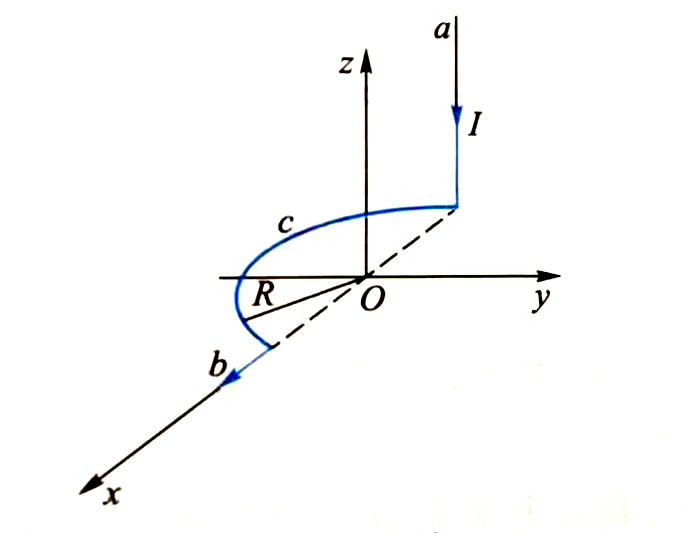
\includegraphics[width=0.35\linewidth]{figure/9-10}
		\caption{图9-10}
		\label{fig:9-10}
	\end{figure}
	
	\item [\textbf{9-12}]
	如习题9-12图所示，AB、CD为长直导线，$\wideparen{BC}$为圆心在$O$点的一段圆弧形导线，其半径为$\mathbf{R}$.若通以电流$\textit{I}$,求$O$点的磁感应强度.
	% TODO: \usepackage{graphicx} required
	\begin{figure}[H]
		\centering
		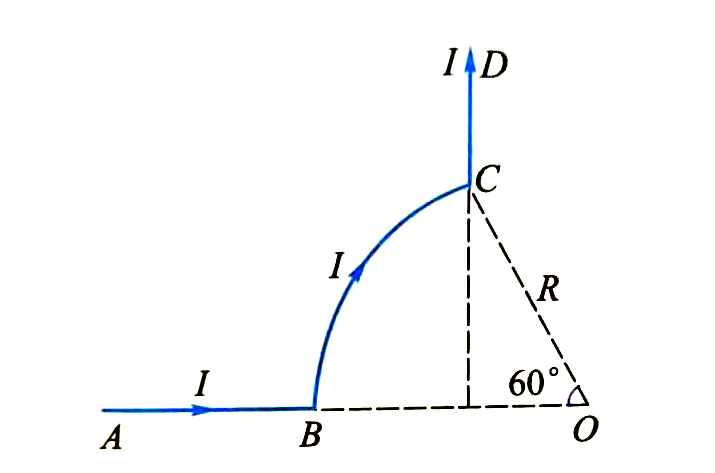
\includegraphics[width=0.35\linewidth]{figure/9-12}
		\caption{图9-12}
		\label{fig:9-12}
	\end{figure}
	
	\item [\textbf{9-15}]
	两平行长直导线相距$\textit{d}=40\,\text{cm}$,每根导线载有电流$\boldsymbol{I}_1=\boldsymbol{I}_2=20A$,如习题9-15图所示.求
	\begin{enumerate}
		\item [(1)] 两导线所在平面内与该两导线等距的一点A处的磁感应强度：
		\item [(2)] 通过图中方框面积的磁通量.($r_1=r_2=10cm,l=25cm.$)
	\end{enumerate}
	% TODO: \usepackage{graphicx} required
	\begin{figure}[H]
		\centering
		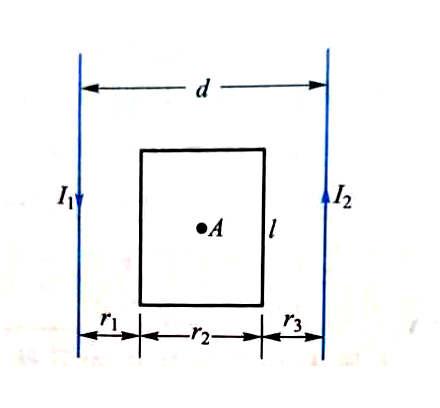
\includegraphics[width=0.3\linewidth]{figure/9-15}
		\caption{图9-15}
		\label{fig:9-15}
	\end{figure}
	
	\item [\textbf{9-16}]
	长直电缆由半径为$\mathbf{R_1}$的导体圆柱与同轴的内外半径分别为$\mathbf{R_2}$、$\mathbf{R_2}$的导体圆筒构成，电流沿轴线方向由一导体流入，从另一导体流出，设电流$\textit{I}$均匀地分布在横截面上。求距轴线为r处的磁感应强度大小$(0<r<\infty)$.
	
	\item [\textbf{9-19}]
	半径为$\textbf{R}$的半圆形闭合线圈，载有电流$\textit{I}$，放在均匀磁场中，磁场方向与线圈平面平行，如习题9‑19图所示。
	\begin{enumerate}
		\item [(1)] 求线圈所受力矩的大小和方向(以直径为转轴)；
		\item [(2)] 若线圈受上述磁场作用转到线圈平面与磁场垂直的位置，则力矩做的功为多少？
	\end{enumerate}
	% TODO: \usepackage{graphicx} required
	\begin{figure}[H]
		\centering
		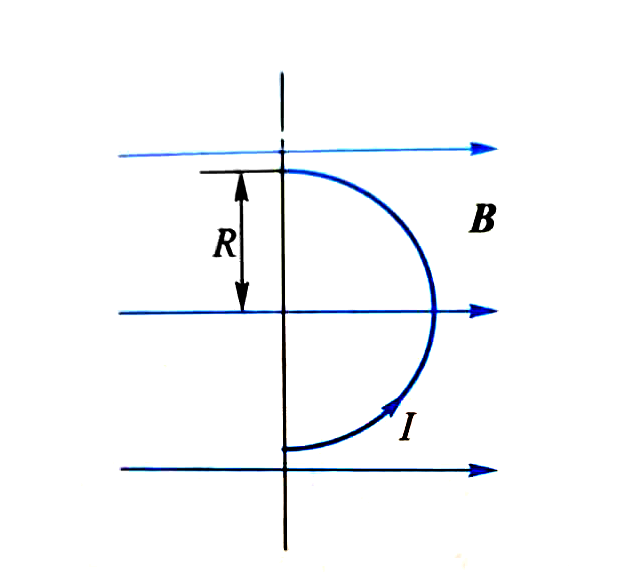
\includegraphics[width=0.3\linewidth]{figure/9-19}
		\caption{图9-19}
		\label{fig:9-19}
	\end{figure}
	
	\item [\textbf{9-20}]
	如习题9-20图所示，在长直导线AB内通以电流$\boldsymbol{I_1}=20A$，在矩形线圈CDEF中通以电流$\boldsymbol{I_2}=10A$，AB与线圈共面，且CD、EF都与AB平行。已知$a=9.0cm,b=20.0cm,d=1.0cm$，求:
	\begin{enumerate}
		\item [(1)] 导线AB的磁场对矩形线圈每边所作用的力；
		\item [(2)] 矩形线圈所受合力和合力矩。
	\end{enumerate}
	% TODO: \usepackage{graphicx} required
	\begin{figure}[H]
		\centering
		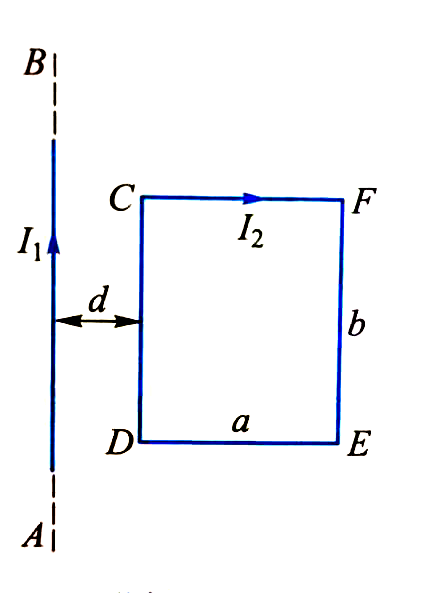
\includegraphics[width=0.25\linewidth]{figure/9-20}
		\caption{图9-20}
		\label{fig:9-20}
	\end{figure}
	
\end{enumerate}

\newpage

\subsection*{习题9题解}

\textbf{9-10题解： }
\setcounter{equation}{0}
\renewcommand{\theHequation}{9-10.\arabic{equation}}

\textbf{答案： }
$B_O = -\frac{\mu_0 I}{4R} \left( \frac{1}{\pi}\vec{j} + \vec{k} \right)$

\textbf{解答过程： }
为了求出坐标原点 $O$ 处的总磁感应强度 $B$，我们依然将导线分为 $a$、$c$、$b$ 三个部分分别计算，最后进行矢量叠加。设 $x,y,z$ 轴的单位矢量分别为 $\vec{i},\vec{j},\vec{k}$。

\textbf{1. 线段 $a$ （半无限长直导线）}
\begin{itemize}
	\item \textbf{几何与位置：} 平行于 $z$ 轴，落在 $x = -R, y = 0$ 处。电流从 $z = +\infty$ 流向 $z = 0$。
	\item \textbf{大小：} 它是一根一端延伸到无穷远、另一端刚好与观测点（原点）平齐的半无限长直导线。它到原点的垂直距离为 $R$。其在原点产生的磁场大小为无限长直导线的一半：
	\begin{equation}\label{eq:9-10-1}
		B_a = \frac{\mu_0 I}{4\pi R}
	\end{equation}
	\item \textbf{方向：} 根据\textbf{右手螺旋定则}，大拇指指向电流方向（向下，即 $-z$ 方向），四指弯曲。在原点 $O$ 处（位于导线的正前方 $+x$ 方向），磁场的切线方向刚好指向 $y$ 轴的负方向。
	\item \textbf{矢量表示：}
	\begin{equation}\label{eq:9-10-2}
		\vec{B}_a = -\frac{\mu_0 I}{4\pi R}\vec{j}
	\end{equation}
\end{itemize}

\textbf{2. 线段 $c$ （半圆弧）}
\begin{itemize}
	\item \textbf{几何与位置：} 位于 $Oxy$ 平面内，从 $x$ 轴负半轴 ($-R, 0, 0$) 出发，经过 $y$ 轴，到达 $x$ 轴正半轴 ($R, 0, 0$) 的半圆。
	\item \textbf{大小：} 完整圆环在圆心产生的磁场为 $\frac{\mu_0 I}{2R}$。因为是半圆，所以磁场大小是其一半：
	\begin{equation}\label{eq:9-10-3}
		B_c = \frac{1}{2} \times \frac{\mu_0 I}{2R} = \frac{\mu_0 I}{4R}
	\end{equation}
	\item \textbf{方向：} 再次使用\textbf{右手螺旋定则}。四指顺着电流方向（从 $-x$ 轴弯向 $+x$ 轴），大拇指垂直于 $Oxy$ 平面向里，即指向 $z$ 轴的负方向。
	\item \textbf{矢量表示：}
	\begin{equation}\label{eq:9-10-4}
		\vec{B}_c = -\frac{\mu_0 I}{4R}\vec{k}
	\end{equation}
\end{itemize}

\textbf{3. 线段 $b$ （沿径向的半无限长直导线）}
\begin{itemize}
	\item \textbf{几何与位置：} 位于 $x$ 轴正半轴上，从 $x = R$ 延伸至 $+\infty$。
	\item \textbf{磁场分析：} 观察点 $O$ 刚好位于该导线的反向延长线上。根据毕奥-萨伐尔定律，此时电流元 $dl$ 的方向与从电流元指向原点的位矢 $r$ 平行，它们的叉乘 $dl \times r = 0$。
	\item \textbf{矢量表示：}
	\begin{equation}\label{eq:9-10-5}
		\vec{B}_b = 0
	\end{equation}
\end{itemize}

\textbf{最终结果：矢量叠加}

根据磁场的叠加原理，$O$ 点的总磁感应强度为这三部分的矢量和：
\begin{equation}\label{eq:9-10-6}
	\vec{B}_O = \vec{B}_a + \vec{B}_c + \vec{B}_b
\end{equation}

代入上面求得的各分量：
\begin{equation}\label{eq:9-10-7}
	\vec{B}_O = -\frac{\mu_0 I}{4\pi R}\vec{j} - \frac{\mu_0 I}{4R}\vec{k}
\end{equation}

为了结果更加清晰，我们可以提取公因式 $\frac{\mu_0 I}{4R}$，写成如下形式：
\begin{equation}\label{eq:9-10-8}
	\vec{B}_O = -\frac{\mu_0 I}{4R} \left( \frac{1}{\pi}\vec{j} + \vec{k} \right)
\end{equation}

\textbf{易混淆知识点： }
1. \textbf{空间坐标系与右手定则的匹配}：在三维空间中，判断直导线磁场方向时，需明确导线所在位置到场点的矢径方向（本题中线段 $a$ 到原点是沿着 $+x$ 方向），结合右手定则才能准确得出磁场沿 $-y$ 方向（$\vec{j}$ 的反向）。

2. \textbf{半圆弧的磁场大小}：圆弧磁场的通用公式为 $B = \frac{\mu_0 I}{4\pi R} \theta$（$\theta$ 为圆心角，代入 $\pi$ 即可得到半圆的 $\frac{\mu_0 I}{4R}$），切忌死记硬背而与四分之一圆弧混淆。

\vspace{1em}

\textbf{9-12题解： }
\setcounter{equation}{0}
\renewcommand{\theHequation}{9-12.\arabic{equation}}

\textbf{答案： }
大小为 $B_O = \frac{\mu_0 I}{2R} \left[ \frac{1}{6} + \frac{1}{\pi} \left( 1 - \frac{\sqrt{3}}{2} \right) \right]$，方向垂直纸面向里（$\otimes$）。

\textbf{解答过程： }
\textbf{1. 线段 $AB$ （水平长直导线）}
\begin{itemize}
	\item 依然为 0。电流延长线穿过 $O$ 点，$d\vec{l} \times \vec{r} = 0$。
\end{itemize}

\textbf{2. 线段 $BC$ （$60^\circ$ 圆弧）}
\begin{itemize}
	\item \textbf{大小：} 既然圆心角是 $60^\circ$，那它就是完整圆（$360^\circ$）的 $\frac{1}{6}$。
	\begin{equation}\label{eq:9-12-1}
		B_{BC} = \frac{1}{6} \times \frac{\mu_0 I}{2R} = \frac{\mu_0 I}{12R}
	\end{equation}
	\item \textbf{方向：} 电流从 $B$ 流向 $C$，也就是绕着 $O$ 点顺时针转动。根据右手螺旋定则，四指顺时针弯曲，大拇指指向纸面向里。设纸面向外为 $\vec{k}$ 轴正向，则：
	\begin{equation}\label{eq:9-12-2}
		\vec{B}_{BC} = -\frac{\mu_0 I}{12R}\vec{k}
	\end{equation}
\end{itemize}

\textbf{3. 线段 $CD$ （竖直长直导线）}
\begin{itemize}
	\item \textbf{几何位置：} 设垂足为 $P$。在直角 $\triangle CPO$ 中，直角边 $OP = R \cos 60^\circ = \frac{R}{2}$。这意味着竖直导线 $CD$ 到观察点 $O$ 的垂直距离 $d = \frac{R}{2}$。并且，\textbf{导线在 $O$ 点的左侧}。
	\item \textbf{大小计算：} 利用直导线公式 $B = \frac{\mu_0 I}{4\pi d}(\sin \theta_2 - \sin \theta_1)$。
	\begin{itemize}
		\item 起点 $C$ 对应的角度 $\theta_1 = 60^\circ$。
		\item 终点延伸至无穷远，$\theta_2 = 90^\circ$。
	\end{itemize}
	\begin{equation}\label{eq:9-12-3}
		B_{CD} = \frac{\mu_0 I}{4\pi (\frac{R}{2})} (\sin 90^\circ - \sin 60^\circ) = \frac{\mu_0 I}{2\pi R} \left( 1 - \frac{\sqrt{3}}{2} \right)
	\end{equation}
	\item \textbf{方向（关键修正）：} 导线 $CD$ 在 $O$ 的左侧，电流方向向上。伸出右手，大拇指朝上，四指在导线的右侧（即 $O$ 点所在位置）会自然地指向\textbf{纸面向里}。
	\begin{equation}\label{eq:9-12-4}
		\vec{B}_{CD} = -\frac{\mu_0 I}{2\pi R} \left( 1 - \frac{\sqrt{3}}{2} \right)\vec{k}
	\end{equation}
\end{itemize}

\textbf{最终正确结果：同向叠加}

因为圆弧和直导线在 $O$ 点产生的磁场方向\textbf{都是向里}的，所以它们不是相减，而是直接相加：
\begin{equation}\label{eq:9-12-5}
	\vec{B}_O = \vec{B}_{BC} + \vec{B}_{CD}
\end{equation}

\begin{equation}\label{eq:9-12-6}
	\vec{B}_O = -\frac{\mu_0 I}{12R}\vec{k} - \frac{\mu_0 I}{2\pi R} \left( 1 - \frac{\sqrt{3}}{2} \right)\vec{k}
\end{equation}

为了美观，提出公因式 $\frac{\mu_0 I}{2R}$ 并去掉负号说明方向：

大小：
\begin{equation}\label{eq:9-12-7}
	B_O = \frac{\mu_0 I}{2R} \left[ \frac{1}{6} + \frac{1}{\pi} \left( 1 - \frac{\sqrt{3}}{2} \right) \right]
\end{equation}

方向：\textbf{垂直纸面向里（$\otimes$）}

\textbf{易混淆知识点： }
1. \textbf{圆心角的判定}：需明确题目给出的 $60^\circ$ 究竟是圆弧与水平线的夹角还是圆弧本身的张角，结合图中修正的逻辑，确认其为完整圆周的 $\frac{1}{6}$。

2. \textbf{磁场方向的相对位置判定}：\textbf{判断直导线磁场方向时，不仅要看电流方向（如向上），还要极其注意场点位于导线的左侧还是右侧。}本题中 $O$ 点位于向上的直导线 $CD$ 的右侧，故磁场向里，导致两部分磁场同向叠加。\textcolor{red}{注意：算完磁场一定要用右手螺旋检查方向！}

\vspace{1em}

\textbf{9-15题解： }
\setcounter{equation}{0}
\renewcommand{\theHequation}{9-15.\arabic{equation}}

\textbf{答案： }
(1) $A$ 点的磁感应强度大小为 $4 \times 10^{-5}\,\text{T}$，方向垂直纸面向外。\\
(2) 通过图中方框面积的磁通量为 $10^{-6} \ln 3\,\text{Wb}$ （约 $1.1 \times 10^{-6}\,\text{Wb}$）。

\textbf{解答过程： }
(1) 由安培环路定理可知，无限长直导线产生的磁场公式为 $B = \frac{\mu_0 I}{2\pi r}$。
根据题意，点 $A$ 与两导线等距，即距每根导线的距离均为 $r_A = \frac{d}{2} = 20\,\text{cm} = 0.2\,\text{m}$。

左侧导线电流 $I_1$ 向下，根据右手螺旋定则，其在右侧 $A$ 点产生的磁感应强度 $\vec{B}_1$ 方向垂直纸面向外，大小为：
\begin{equation}\label{eq:9-15-1}
	B_1 = \frac{\mu_0 I_1}{2\pi (d/2)}
\end{equation}

右侧导线电流 $I_2$ 向上，根据右手螺旋定则，其在左侧 $A$ 点产生的磁感应强度 $\vec{B}_2$ 方向也垂直纸面向外，大小为：
\begin{equation}\label{eq:9-15-2}
	B_2 = \frac{\mu_0 I_2}{2\pi (d/2)}
\end{equation}

由于 $\vec{B}_1$ 和 $\vec{B}_2$ 方向相同，根据磁场叠加原理，$A$ 点的总磁感应强度 $B_A$ 为两者的代数和。代入 $I_1 = I_2 = 20\,\text{A}$ 以及 $d = 0.4\,\text{m}$：
\begin{align*}
	B_A &= B_1 + B_2 = 2 \times \frac{4\pi \times 10^{-7} \times 20}{2\pi \times 0.2} \\
	&= 4 \times 10^{-5}\,\text{T}
\end{align*}
方向垂直纸面向外。

(2) 建立坐标系，设左侧导线所在直线为 $y$ 轴，$x$ 轴水平向右。
在距左导线距离为 $x$ 处，取宽为 $\mathrm{d}x$、长为 $l$ 的竖直狭长面元 $\mathrm{d}S = l \mathrm{d}x$。
该处的磁场由两根导线共同产生，且方向均垂直纸面向外，其大小为：
\begin{equation}\label{eq:9-15-3}
	B(x) = \frac{\mu_0 I_1}{2\pi x} + \frac{\mu_0 I_2}{2\pi (d-x)} = \frac{\mu_0 I}{2\pi} \left( \frac{1}{x} + \frac{1}{d-x} \right)
\end{equation}

穿过该狭长面元的微小磁通量为 $\mathrm{d}\Phi = B(x) \mathrm{d}S = B(x) l \mathrm{d}x$。
根据图中尺寸，方框的左边界坐标为 $x = r_1 = 10\,\text{cm} = 0.1\,\text{m}$，右边界坐标为 $x = r_1 + r_2 = 20\,\text{cm} = 0.2\,\text{m}$。
对方框面积进行定积分求总磁通量：
\begin{align*}
	\Phi &= \int_{r_1}^{r_1+r_2} B(x) l \mathrm{d}x \\
	&= \int_{0.1}^{0.2} \frac{\mu_0 I l}{2\pi} \left( \frac{1}{x} + \frac{1}{0.4-x} \right) \mathrm{d}x \\
	&= \frac{\mu_0 I l}{2\pi} \left[ \ln x - \ln(0.4-x) \right]_{0.1}^{0.2} \\
	&= \frac{\mu_0 I l}{2\pi} \left[ \ln\left(\frac{x}{0.4-x}\right) \right]_{0.1}^{0.2}
\end{align*}

代入上下限（$I = 20\,\text{A}, l = 0.25\,\text{m}$）：
\begin{align*}
	\Phi &= \frac{4\pi \times 10^{-7} \times 20 \times 0.25}{2\pi} \left( \ln\left(\frac{0.2}{0.2}\right) - \ln\left(\frac{0.1}{0.3}\right) \right) \\
	&= 2 \times 10^{-7} \times 5 \times (\ln 1 - \ln\frac{1}{3}) \\
	&= 10^{-6} \ln 3 \,\text{Wb} \approx 1.098 \times 10^{-6} \,\text{Wb}
\end{align*}

\textbf{易混淆知识点： }
1. \textbf{右手螺旋定则与磁场叠加}：两根导线电流方向相反（一上一下），直觉上有时会误以为它们在中间区域产生的磁场会相互抵消。实际上，\textbf{画一下磁感线就会发现，向下电流在右侧产生的磁场向外，向上电流在左侧产生的磁场也向外}，两者在连线中间区域是\textbf{相互加强}的。\textcolor{red}{一定要学会用右手螺旋定则来判断方向，不要死记硬背！}

2. \textbf{积分区间的坐标对应}：在第二问求磁通量时，图中标注了 $r_1, r_2, r_3$。在代入积分上限时，极易将上限错误地写成 $r_2=0.1$。实际上 $r_2$ 表示的是方框的“宽度”，如果以左侧导线为坐标原点，积分变量 $x$ 应当从方框左边界（$x=r_1=0.1$）一直积到右边界（$x=r_1+r_2=0.2$）。

\vspace{1em}

\textbf{9-16题解： }(\textcolor{red}{本题最后附上了理解图，极易解决抽象问题。})
\setcounter{equation}{0}
\renewcommand{\theHequation}{9-16.\arabic{equation}}

\textbf{答案： }
距轴线为 $r$ 处的磁感应强度大小分布如下：\\
(1) $0 \le r < R_1$ 时，$B = \frac{\mu_0 I r}{2\pi R_1^2}$；\\
(2) $R_1 \le r < R_2$ 时，$B = \frac{\mu_0 I}{2\pi r}$；\\
(3) $R_2 \le r < R_3$ 时，$B = \frac{\mu_0 I}{2\pi r} \frac{R_3^2 - r^2}{R_3^2 - R_2^2}$；\\
(4) $r \ge R_3$ 时，$B = 0$。

\textbf{解答过程： }
根据安培环路定理：
\begin{equation}\label{eq:9-16-1}
	\oint_L \vec{B} \cdot \mathrm{d}\vec{l} = \mu_0 \sum I_{\text{内}}
\end{equation}
由电缆的轴对称性可知，磁场方向垂直于径向且与轴线共面分布，磁感线为以轴线为圆心的同心圆。取半径为 $r$ 的同心圆作为积分回路，则左侧环流恒为 $B \cdot 2\pi r$。

(1) 在内部导体内（$0 \le r < R_1$）：
内部导体中电流均匀分布，电流密度 $J_1 = \frac{I}{\pi R_1^2}$。
积分回路包围的电流为：
\begin{align*}
	\sum I_{\text{内}} = J_1 \cdot \pi r^2 = I \frac{r^2}{R_1^2}
\end{align*}
代入安培环路定理得 $B \cdot 2\pi r = \mu_0 I \frac{r^2}{R_1^2}$，解得：
\begin{equation}\label{eq:9-16-2}
	B = \frac{\mu_0 I r}{2\pi R_1^2}
\end{equation}

(2) 在两导体之间（$R_1 \le r < R_2$）：
积分回路包围的电流为整个内部导体的电流：
\begin{align*}
	\sum I_{\text{内}} = I
\end{align*}
代入安培环路定理得 $B \cdot 2\pi r = \mu_0 I$，解得：
\begin{equation}\label{eq:9-16-3}
	B = \frac{\mu_0 I}{2\pi r}
\end{equation}

(3) 在外部导体圆筒内（$R_2 \le r < R_3$）：
外部圆筒中的电流与内部电流方向相反，外部圆筒的电流密度 $J_2 = \frac{I}{\pi (R_3^2 - R_2^2)}$。
积分回路包围的总电流等于内部导体正向电流减去外部圆筒被包围部分的反向电流：
\begin{align*}
	\sum I_{\text{内}} &= I - J_2 \cdot \pi (r^2 - R_2^2) \\
	&= I - I \frac{r^2 - R_2^2}{R_3^2 - R_2^2} \\
	&= I \frac{R_3^2 - r^2}{R_3^2 - R_2^2}
\end{align*}
代入安培环路定理得 $B \cdot 2\pi r = \mu_0 I \frac{R_3^2 - r^2}{R_3^2 - R_2^2}$，解得：
\begin{equation}\label{eq:9-16-4}
	B = \frac{\mu_0 I}{2\pi r} \frac{R_3^2 - r^2}{R_3^2 - R_2^2}
\end{equation}

(4) 在电缆外部（$r \ge R_3$）：
积分回路包围的总电流为内外两导体电流之和（一进一出，大小相等）：
\begin{align*}
	\sum I_{\text{内}} = I - I = 0
\end{align*}
代入安培环路定理得：
\begin{equation}\label{eq:9-16-5}
	B = 0
\end{equation}

\textbf{易混淆知识点： }
1. \textbf{外部圆筒区域包围电流的计算}：在 $R_2 \le r < R_3$ 区域求 $\sum I_{\text{内}}$ 时，很多人会错误地只计算外部圆筒本身的电流而忘记加上内层导体的总电流 $I$；或者是计算外层包围面积时用 $\pi r^2$ 减去内层圆的面积。\textbf{务必记住，外层截面积是圆环形 $\pi(R_3^2 - R_2^2)$，被包围的外层面积是 $\pi(r^2 - R_2^2)$。}

2. \textbf{同轴电缆的磁屏蔽效应}：由第(4)问结果可知，对于电流等大反向的同轴电缆，其外部空间磁场严格为零。这是同轴电缆被广泛应用于抗干扰信号传输的物理本质。

% TODO: \usepackage{graphicx} required
\begin{figure}[H]
	\centering
	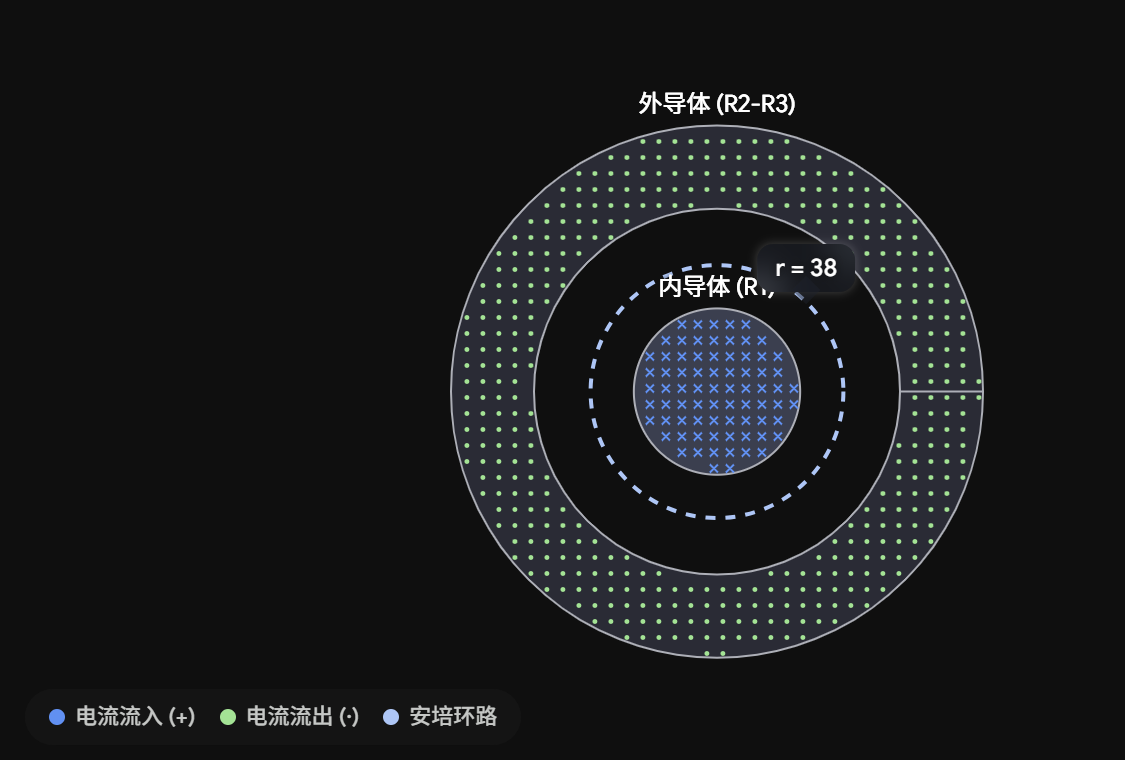
\includegraphics[width=0.6\linewidth]{figure/9-16}
	\caption{9-16辅助做题图}
	\label{fig:9-16}
\end{figure}


\vspace{1em}

\textbf{9-19题解： }
\setcounter{equation}{0}
\renewcommand{\theHequation}{9-19.\arabic{equation}}

\textbf{答案： }
(1) 线圈所受力矩的大小为 $\tau = \frac{1}{2}\pi R^2 I B$，方向为沿直导线向上（$+y$ 轴方向）。\\
(2) 力矩做的功为 $A = \frac{1}{2}\pi R^2 I B$。

\textbf{解答过程： }
为了推导的绝对严谨（明确几何方位对这类题非常重要），我们先建立一个清晰的直角坐标系：
\begin{itemize}
	\item 直线段的直边（直径）与 $y$ 轴重合，中点为原点 $O$。
	\item 半圆弧线圈初始处于 $Oxy$ 平面的右侧（$x \ge 0$ 区域）。
	\item 匀强磁场水平向右，即沿 $+x$ 轴方向，表示为 $\mathbf{B} = B\mathbf{i}$。
	\item 观察图中半圆弧下方的箭头，假设电流 $I$ 沿着弧线是由下而上流动的，顺着直边自上而下流回。这是一个逆时针方向的闭合回路。
\end{itemize}

\textbf{(1) 求线圈所受力矩的大小和方向}

在期末考试中，处理任意形状的平面闭合线圈受力矩问题，“等效磁矩法”是最快捷且不容易出错的方法。

\textbf{步骤 1：计算线圈的磁矩 $\mathbf{p}_m$}

闭合线圈的磁矩定义为 $\mathbf{p}_m = I S \mathbf{n}$。
\begin{itemize}
	\item \textbf{面积 $S$：} 半圆的面积为 $S = \frac{1}{2}\pi R^2$。
	\item \textbf{法向量 $\mathbf{n}$ 的方向：} 使用右手螺旋定则，四指顺着逆时针的电流方向弯曲，大拇指指向纸面向外，即 $+z$ 轴方向，$\mathbf{n} = \mathbf{k}$。
	\item 因此，初始状态下的磁矩矢量为：
\end{itemize}
\begin{equation}\label{eq:9-19-1}
	\mathbf{p}_m = \frac{1}{2}\pi R^2 I \mathbf{k}
\end{equation}

\textbf{步骤 2：利用叉乘公式求力矩 $\boldsymbol{\tau}$}

处于均匀磁场中的载流线圈，其受到的磁力矩公式为 $\boldsymbol{\tau} = \mathbf{p}_m \times \mathbf{B}$。(\textcolor{red}{注意：这个磁力矩公式其实还要乘以$\sin\theta$,这里是因为磁力矩垂直向外，B向右，所以$\theta$=90°})代入我们建立的矢量：
\begin{align*}
	\boldsymbol{\tau} &= \left( \frac{1}{2}\pi R^2 I \mathbf{k} \right) \times (B\mathbf{i}) \\
	&= \frac{1}{2}\pi R^2 I B (\mathbf{k} \times \mathbf{i})
\end{align*}
由于 $\mathbf{k} \times \mathbf{i} = \mathbf{j}$，所以：
\begin{equation}\label{eq:9-19-2}
	\boldsymbol{\tau} = \frac{1}{2}\pi R^2 I B \mathbf{j}
\end{equation}

\textbf{结论：}
\begin{itemize}
	\item \textbf{大小：} $\tau = \frac{1}{2}\pi R^2 I B$
	\item \textbf{方向：} 沿 $+y$ 轴方向（即沿直导线向上）。物理上的直观体现是：这个力矩会迫使半圆形线圈向纸面外翻转，以直边为转轴转动。
\end{itemize}

\textbf{(2) 求转到与磁场垂直位置时，力矩做的功}

力矩做功的本质是线圈的磁势能转化成了动能或其他形式的能。我们可以直接利用磁势能的公式来计算，这比计算力矩的积分要简便得多。
\textbf{线圈在磁场中的势能公式为}：
\begin{equation}\label{eq:9-19-3}
	W_p = -\mathbf{p}_m \cdot \mathbf{B} = -p_m B \cos\theta
\end{equation}
（其中 $\theta$ 是磁矩 $\mathbf{p}_m$ 与磁场 $\mathbf{B}$ 的夹角）

\textbf{步骤 1：确定初始状态的势能 $W_{p1}$}

初始时，线圈平面与磁场平行，这意味着线圈的法向量（磁矩 $\mathbf{p}_m$）与磁场 $\mathbf{B}$ 垂直。
$$ \theta_1 = 90^\circ $$
\begin{equation}\label{eq:9-19-4}
	W_{p1} = -p_m B \cos 90^\circ = 0
\end{equation}

\textbf{步骤 2：确定末状态的势能 $W_{p2}$}

当线圈在力矩的作用下自由转动到与磁场垂直的位置时，它是在向“稳定平衡状态”趋近。此时磁矩 $\mathbf{p}_m$ 会与磁场 $\mathbf{B}$ 的方向完全一致（同向）。
$$ \theta_2 = 0^\circ $$
\begin{equation}\label{eq:9-19-5}
	W_{p2} = -p_m B \cos 0^\circ = -p_m B = -\frac{1}{2}\pi R^2 I B
\end{equation}

\textbf{步骤 3：计算磁场力做功 $A$}

做功等于系统势能的减少量（$A = -\Delta W_p = W_{p1} - W_{p2}$）：
\begin{align*}
	A &= 0 - \left( -\frac{1}{2}\pi R^2 I B \right) \\
	&= \frac{1}{2}\pi R^2 I B
\end{align*}

\textbf{结论：}
力矩在此过程中做的正功为 $\frac{1}{2}\pi R^2 I B$。

\vspace{1em}

\textbf{9-20题解： }
\setcounter{equation}{0}
\renewcommand{\theHequation}{9-20.\arabic{equation}}

\textbf{答案： }
(1) 导线 AB 的磁场对矩形线圈每边所作用的力分别为：

左侧边 CD 受力大小为 $8.0 \times 10^{-4}\,\text{N}$，方向水平向左；

右侧边 FE 受力大小为 $8.0 \times 10^{-5}\,\text{N}$，方向水平向右；

上侧边 CF 受力大小约为 $9.21 \times 10^{-5}\,\text{N}$，方向竖直向上；

下侧边 DE 受力大小约为 $9.21 \times 10^{-5}\,\text{N}$，方向竖直向下。\\
(2) 矩形线圈所受合力大小为 $7.2 \times 10^{-4}\,\text{N}$，方向水平向左（指向导线 AB）；合力矩为 $0$。

\textbf{解答过程： }
(1) 建立直角坐标系，设长直导线 AB 所在直线为 $y$ 轴，向右为 $x$ 轴正方向。
由安培环路定理可知，长直导线 AB 在其右侧距离为 $x$ 处产生的磁感应强度大小为：
\begin{equation}\label{eq:9-20-1}
	B(x) = \frac{\mu_0 I_1}{2\pi x}
\end{equation}
根据右手螺旋定则，线圈所在平面的磁场方向均\textbf{垂直于纸面向里}。
已知各参数为：$I_1 = 20\,\text{A}, I_2 = 10\,\text{A}, a = 0.09\,\text{m}, b = 0.20\,\text{m}, d = 0.01\,\text{m}, \mu_0 = 4\pi \times 10^{-7}\,\text{T}\cdot\text{m/A}$。

\textbf{对于左侧边 CD：}
该边距离直导线 $x = d$，所在处的磁场是均匀的。电流方向向上（与 $I_1$ 同向）。
受到的安培力大小为：
\begin{align*}
	F_{CD} &= I_2 b B(d) = \frac{\mu_0 I_1 I_2 b}{2\pi d} \\
	&= \frac{4\pi \times 10^{-7} \times 20 \times 10 \times 0.20}{2\pi \times 0.01} \\
	&= 8.0 \times 10^{-4}\,\text{N}
\end{align*}
根据左手定则（或同向电流相吸原理），方向为\textbf{水平向左}。

\textbf{对于右侧边 FE：}
该边距离直导线 $x = d + a = 0.10\,\text{m}$，磁场均匀。电流方向向下（与 $I_1$ 反向）。
受到的安培力大小为：
\begin{align*}
	F_{FE} &= I_2 b B(d+a) = \frac{\mu_0 I_1 I_2 b}{2\pi (d+a)} \\
	&= \frac{4\pi \times 10^{-7} \times 20 \times 10 \times 0.20}{2\pi \times 0.10} \\
	&= 8.0 \times 10^{-5}\,\text{N}
\end{align*}
根据左手定则（或反向电流相斥原理），方向为\textbf{水平向右}。

\textbf{对于上侧边 CF：}
该边各点到 AB 的距离 $x$ 随位置变化，磁场为非匀强磁场，需使用微元法积分。
在距离 AB 为 $x$ 处取微元 $\mathrm{d}x$，其受力为 $\mathrm{d}F = I_2 \mathrm{d}x B(x)$。
电流方向向右，磁场向里，由左手定则知各微元受力均向上。总安培力为：
\begin{align*}
	F_{CF} &= \int_{d}^{d+a} I_2 B(x) \mathrm{d}x = \int_{d}^{d+a} \frac{\mu_0 I_1 I_2}{2\pi x} \mathrm{d}x \\
	&= \frac{\mu_0 I_1 I_2}{2\pi} \ln\left(\frac{d+a}{d}\right) \\
	&= \frac{4\pi \times 10^{-7} \times 20 \times 10}{2\pi} \ln\left(\frac{0.10}{0.01}\right) \\
	&= 4 \times 10^{-5} \ln 10 \approx 9.21 \times 10^{-5}\,\text{N}
\end{align*}
方向为\textbf{竖直向上}。

\textbf{对于下侧边 DE：}
与上侧边对称，电流方向向左，磁场向里，受力方向\textbf{竖直向下}。大小与 CF 边完全相等：
\begin{equation}\label{eq:9-20-2}
	F_{DE} = F_{CF} \approx 9.21 \times 10^{-5}\,\text{N}
\end{equation}

(2) \textbf{求合力：}
\textcolor{red}{上、下两边受力大小相等、方向相反（且作用在同一条竖直线上），相互抵消}：$\vec{F}_{CF} + \vec{F}_{DE} = 0$。
左、右两边受力均在水平方向上，合力大小为：
\begin{align*}
	F_{\text{合}} &= F_{CD} - F_{FE} \\
	&= 8.0 \times 10^{-4} - 0.8 \times 10^{-4} \\
	&= 7.2 \times 10^{-4}\,\text{N}
\end{align*}
由于指向左侧的力较大，合力方向为\textbf{水平向左}。

\textbf{求合力矩：}
矩形线圈中的\textbf{电流为顺时针方向}，由\textbf{右手螺旋定则}可知，该线圈的磁矩 $\vec{p}_m$ 方向为\textbf{垂直于纸面向里}。
而长直导线 AB 在线圈所在区域产生的磁场 $\vec{B}$ 方向也为\textbf{垂直于纸面向里}。
因为磁矩 $\vec{p}_m$ 与外磁场 $\vec{B}$ 的方向相互平行(\textcolor{red}{$\theta=0°$,所以$\sin\theta=0$})，根据磁力矩公式：
\begin{equation}\label{eq:9-20-3}
	\vec{M} = \vec{p}_m \times \vec{B} = 0
\end{equation}
所以线圈所受的合力矩为 $0$。

\textbf{易混淆知识点： }
1. \textbf{非匀强磁场中的安培力计算}：对于平行于直导线的 CD、FE 边，它们处于等距的匀强磁场线上，可以直接用公式 $F=BIL$ 计算；\textbf{但对于垂直于直导线的 CF、DE 边，磁感应强度 $B$ 随距离 $x$ 呈反比衰减，绝不能直接代入某个定值 $B$，必须写出微元 $\mathrm{d}F = I \mathrm{d}x B(x)$ 后进行定积分求和。}

2. \textbf{合力与合力矩的区别}：本题中线圈所受\textbf{合力不为零（存在向左的平移趋势）}，但\textbf{合力矩为零（不存在翻转趋势）}。许多人在求力矩时试图去寻找转轴并分别计算四个力的力臂，这极易出错。直接利用处于匀强或非匀强磁场中平面线圈的统一力矩公式 $\vec{M} = \vec{p}_m \times \vec{B} · \sin\theta$，通过判断磁矩法向量与磁场矢量的共线关系，可以秒杀绝大多数力矩判断题。

\newpage

\subsection{习题10}
\begin{enumerate}
	\item [\textbf{10-20}] 有两根相距为$a$的无限场平行直导线，它们通以大小相等流向相反的电流，且电流均以$\frac{\mathrm{d}I}{\mathrm{d}t}$的变化率增长，若有一边长为$a$的正方形线圈与两导线处于同一平面内，如习题10-20图所示，求线圈中的感应电动势.
	% TODO: \usepackage{graphicx} required
	\begin{figure}[H]
		\centering
		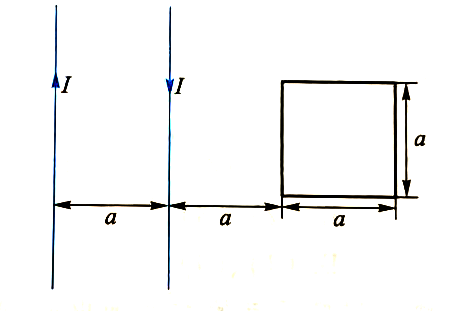
\includegraphics[width=0.33\linewidth]{figure/10-20}
		\caption{图10-20}
		\label{fig:10-20}
	\end{figure}
	
	\item [\textbf{10-22}] 如习题10‑22图所示，在一无限长直导线附近放置一个矩形导线线框，该线框在垂直于导线方向上以匀速度$\boldsymbol{v}$向右移动，求在图示位置处线框中感应电动势的大小和方向。
	% TODO: \usepackage{graphicx} required
	\begin{figure}[H]
		\centering
		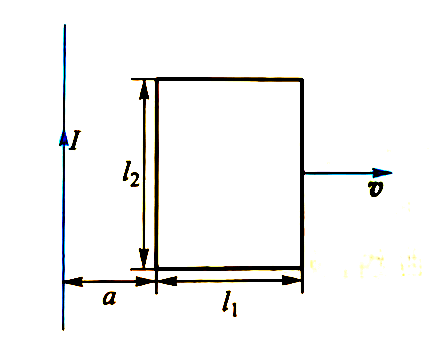
\includegraphics[width=0.3\linewidth]{figure/10-22}
		\caption{图10-22}
		\label{fig:10-22}
	\end{figure}
	
	\item [\textbf{10-23}] 导线ab长为l，绕过O点的垂直轴以匀角速$\boldsymbol{\omega}$转动，$aO=\boldsymbol{\frac{1}{3}l}$，磁感应强度$\boldsymbol{B}$平行于转轴，如习题10‑23图所示，求：
	\begin{itemize}
		\item [(1)] ab两端的电势差；
		\item [(2)] ab两端哪端电势较高？
	\end{itemize}
	% TODO: \usepackage{graphicx} required
	\begin{figure}[H]
		\centering
		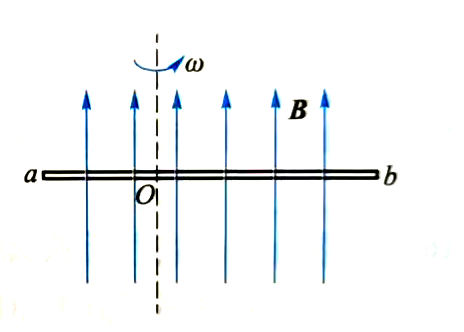
\includegraphics[width=0.4\linewidth]{figure/10-23}
		\caption{图10-23}
		\label{fig:10-23}
	\end{figure}
	
\end{enumerate}

\newpage

\subsection{习题11}
\begin{enumerate}
	\item [\textbf{11-27}] 用白光照射杨氏双缝，已知 $d=1.0\,\mathrm{mm}$，$D=1.0\,\mathrm{m}$，设屏无限大。求：
	\begin{itemize}
		\item [(1)] $\lambda=500\,\mathrm{nm}$ 的光第 $4$ 级明条纹位置及明条纹间距；
		\item [(2)] 求 $\lambda=600\,\mathrm{nm}$ 的光理论上在屏上可呈现的最大级数；
		\item [(3)] $\lambda=500\,\mathrm{nm}$ 和 $\lambda=600\,\mathrm{nm}$ 的光在屏上什么位置开始发生重叠？
	\end{itemize}
	
	\vspace{0.5em}
	
	\item [\textbf{11-43}] 波长 $\lambda=600\,\mathrm{nm}$ 的单色光垂直入射到宽度为 $a=0.01\,\mathrm{mm}$ 的单缝上，观察夫琅禾费衍射图样；透镜焦距 $f=1.0\,\mathrm{m}$，屏幕在透镜的焦平面处，求：
	\begin{itemize}
		\item [(1)] 屏上中央明条纹的宽度 $\Delta x_0$ 和半角宽度；
		\item [(2)] 第二级暗纹所对应的衍射角 $\theta_2$；
		\item [(3)] 第二级暗纹离透镜焦点的距离 $x_2$。
	\end{itemize}
	
	\vspace{0.5em}
	
	\item [\textbf{11-44}] 波长为 $680\,\mathrm{nm}$ 的单色可见光垂直入射到缝宽为 $a=1.25\times 10^{-4}\,\mathrm{cm}$ 的透射光栅上，观察到第四级谱线缺级。求：
	\begin{itemize}
		\item [(1)] 此光栅每厘米有多少条狭缝？
		\item [(2)] 求在屏上呈现的光谱线的全部级次和条纹数。
	\end{itemize}
	
	\vspace{0.5em}
	
	\item [\textbf{11-45}] 波长 $\lambda_1$ 的光与波长 $\lambda_2=486.1\,\mathrm{nm}$ 的光均为平行光，它们同时垂直入射到光栅上。若 $\lambda_1$ 光的第三级光谱线与 $\lambda_2$ 光的第四级光谱线恰好重合在离中央明条纹距离为 $5\,\mathrm{mm}$ 处，透镜焦距为 $0.50\,\mathrm{m}$，求：
	\begin{itemize}
		\item [(1)] $\lambda_1$ 的值；
		\item [(2)] 光栅常量。
	\end{itemize}
	
	\vspace{0.5em}
	
	\item [\textbf{11-47}] 波长为 $600\,\mathrm{nm}$ 的单色光垂直入射到一光栅上，第二和第三主明条纹分别出现在 $\sin\theta_2=0.20$ 和 $\sin\theta_3=0.30$ 处，第四级缺级。问：
	\begin{itemize}
		\item [(1)] 光栅常量是多少？
		\item [(2)] 狭缝最小可能宽度有多大？
		\item [(3)] 按上述选定的 $a,b$ 值，实际呈现的全部级次缺级有哪些？
	\end{itemize}
	
\end{enumerate}

\newpage

\section{课本例题重现}

\subsection*{声明：}

课本例题重现由于期末考机制问题，将只整理一、七、八、九、十、十一章。\textcolor{red}{特别强调：七、八、九、十、十一章为老师勾画的例题极为重要，七八两张的例题一定要复习！}

\subsection{第一章}

\begin{enumerate}
	\item [\textbf{L1-2}]
	\setcounter{equation}{0}
	\renewcommand{\theHequation}{L1-2.\arabic{equation}}
	如图 1-6 所示，一人通过一根不可伸缩的绳水平向右拉小车前进，绳跨过一个小定滑轮，小车位于人拉绳的一端上方高为 $h$ 的平台上，人的速率 $v_0$ 不变，求人离滑轮的水平距离为 $s$ 时，小车的速度大小和加速度大小。
	
	% TODO: \usepackage{graphicx} required
	\begin{figure}[H]
		\centering
		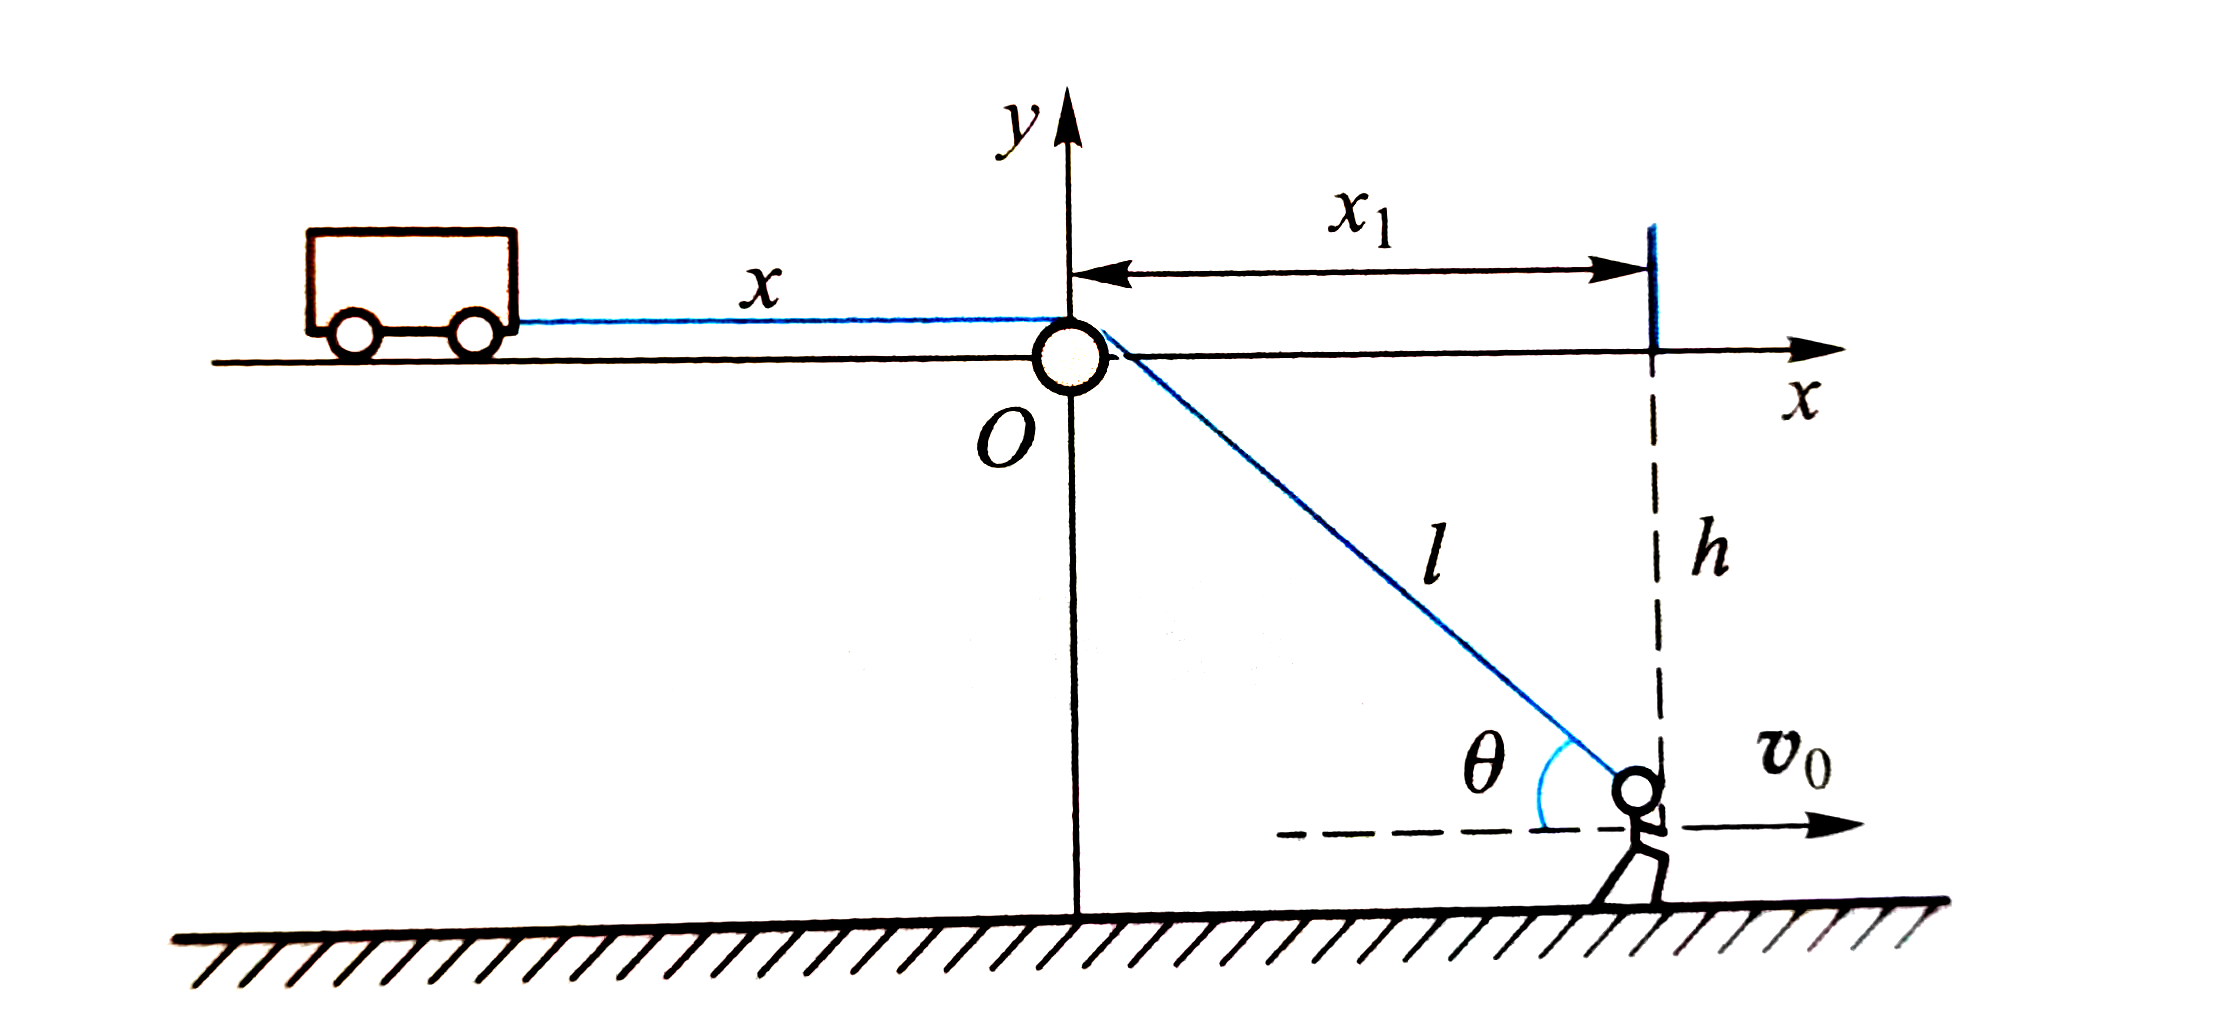
\includegraphics[width=0.4\linewidth]{figure/L1-2}
		\caption{图1-6}
		\label{fig:l1-2}
	\end{figure}
	
	
	\textbf{解} \quad 小车水平向右做直线运动，小车做平动，可看成质点，以地面为参考系，以滑轮处为坐标原点，水平向右为 $x$ 轴正向，竖直向上为 $y$ 轴正向，建立平面直角坐标系. 任意时刻小车的坐标 $(x, y)$ 为 $(x, 0)$（此处 $x < 0$），人的坐标 $(x, y)$ 为 $(x_1, -h)$，小车和人的 $y$ 坐标都是常量. 由速度的定义，小车的速度为
	\begin{align*}
		\boldsymbol{v} = \frac{\mathrm{d}x}{\mathrm{d}t}\boldsymbol{i} + \frac{\mathrm{d}y}{\mathrm{d}t}\boldsymbol{j} = \frac{\mathrm{d}x}{\mathrm{d}t}\boldsymbol{i}
	\end{align*}
	所以小车的速度沿 $x$ 轴方向. 人的速度为
	\begin{align*}
		\boldsymbol{v}_0 = \frac{\mathrm{d}x_1}{\mathrm{d}t}\boldsymbol{i} + \frac{\mathrm{d}y}{\mathrm{d}t}\boldsymbol{j} = \frac{\mathrm{d}x_1}{\mathrm{d}t}\boldsymbol{i}
	\end{align*}
	已知人的速度 $\boldsymbol{v}_0 = v_0\boldsymbol{i}$，所以有
	\begin{equation}\label{eq:L1-2-1}
		\frac{\mathrm{d}x_1}{\mathrm{d}t} = v_0
	\end{equation}
	
	又因为绳不可伸缩，设绳总长为 $l_0$，定滑轮和人之间的绳长为 $l$，则有 $l_0 = l + |x| = l - x$，所以
	\begin{equation}\label{eq:L1-2-2}
		x = l - l_0 = \sqrt{x_1^2 + h^2} - l_0
	\end{equation}
	因此，小车的速度为
	\begin{equation}\label{eq:L1-2-3}
		\boldsymbol{v} = \frac{\mathrm{d}x}{\mathrm{d}t}\boldsymbol{i} = \frac{\mathrm{d}}{\mathrm{d}t}\left(\sqrt{x_1^2 + h^2} - l_0\right)\boldsymbol{i} = \frac{\mathrm{d}\left(\sqrt{x_1^2 + h^2} - l_0\right)}{\mathrm{d}x_1} \cdot \frac{\mathrm{d}x_1}{\mathrm{d}t}\boldsymbol{i} = \frac{x_1 v_0}{\sqrt{x_1^2 + h^2}}\boldsymbol{i}
	\end{equation}
	故当人离滑轮的水平距离为 $s$ 时，即 $x_1 = s$ 时，小车的速度大小为 $v = \frac{s v_0}{\sqrt{s^2 + h^2}}$，方向水平向右.
	
	将式（\ref{eq:L1-2-3}）的任意时刻的速度 $\boldsymbol{v}$ 再对时间求导，并利用式（\ref{eq:L1-2-1}），可得小车的加速度为
	\begin{equation}\label{eq:L1-2-4}
		\boldsymbol{a} = \frac{\mathrm{d}\boldsymbol{v}}{\mathrm{d}t} = \frac{\mathrm{d}}{\mathrm{d}t}\left( \frac{x_1 v_0}{\sqrt{x_1^2 + h^2}} \right)\boldsymbol{i} = \frac{\mathrm{d}}{\mathrm{d}x_1}\left( \frac{x_1 v_0}{\sqrt{x_1^2 + h^2}} \right) \cdot \frac{\mathrm{d}x_1}{\mathrm{d}t}\boldsymbol{i} = \frac{h^2 v_0^2}{\left(x_1^2 + h^2\right)^{\frac{3}{2}}}\boldsymbol{i}
	\end{equation}
	小车的加速度方向水平向右，小车做变加速运动，当人离滑轮的水平距离为 $s$ 时，加速度大小为
	\begin{equation}\label{eq:L1-2-5}
		a = \frac{h^2 v_0^2}{\left(s^2 + h^2\right)^{\frac{3}{2}}}
	\end{equation}
	
	\vspace{2em}
	
	\item [\textbf{L1-3}]
	\setcounter{equation}{0}
	\renewcommand{\theHequation}{L1-3.\arabic{equation}}
	\quad 以速度 $v_0$ 平抛一小球，不计空气阻力，如图 1-12 所示. 以平抛时为计时起点，求 $t$ 时刻小球的切向加速度分量 $a_t$ 和法向加速度分量 $a_n$，以及轨迹的曲率半径 $\rho$.
	
	% TODO: \usepackage{graphicx} required
	\begin{figure}[H]
		\centering
		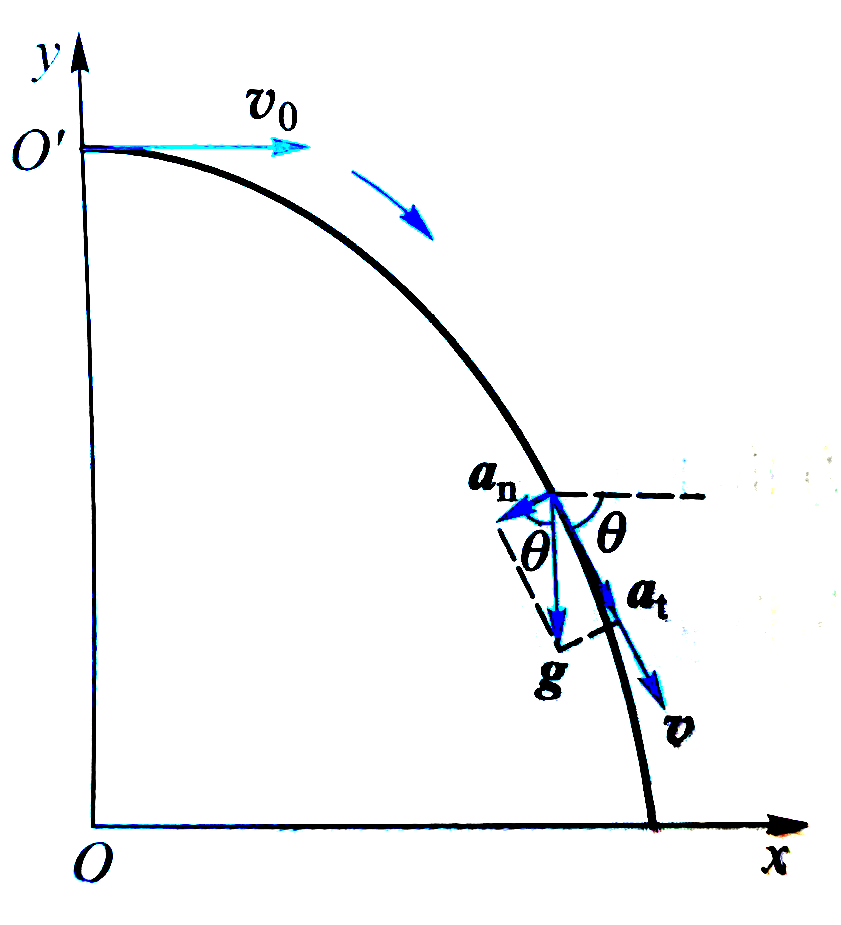
\includegraphics[width=0.3\linewidth]{figure/L1-3}
		\caption{图1-12}
		\label{fig:l1-3}
	\end{figure}
	
	
	\textbf{解一} \quad 建立如图 1-12 所示直角坐标系. 任意 $t$ 时刻，小球的加速度即重力加速度 $g$，方向竖直向下，大小不变. 而任意时刻 $t$，小球速度的 $x, y$ 分量分别为
	\begin{equation}\label{eq:L1-3-1}
		v_x = v_0, \quad v_y = gt
	\end{equation}
	故任意时刻，速度矢量与 $x$ 轴正向之间的夹角 $\theta$（即重力加速度 $g$ 与法向加速度之间的夹角）满足
	\begin{equation}\label{eq:L1-3-2}
		\tan \theta = \frac{v_y}{v_x} = \frac{gt}{v_0}
	\end{equation}
	所以，法向加速度分量为
	\begin{equation}\label{eq:L1-3-3}
		a_n = g \cos \theta = g \frac{v_0}{v} = \frac{g v_0}{\sqrt{v_0^2 + g^2 t^2}}
	\end{equation}
	切向加速度分量为
	\begin{equation}\label{eq:L1-3-4}
		a_t = g \sin \theta = g \frac{gt}{v} = \frac{g^2 t}{\sqrt{v_0^2 + g^2 t^2}}
	\end{equation}
	轨迹的曲率半径为
	\begin{equation}\label{eq:L1-3-5}
		\rho = \frac{v^2}{a_n} = \frac{\left(v_0^2 + g^2 t^2\right)^{3/2}}{g v_0}
	\end{equation}
	
	\textbf{解二} \quad 以抛出点 $O'$ 为自然坐标的原点，建立如图 1-12 所示自然坐标系. 任意 $t$ 时刻，小球速度的 $x, y$ 分量和速率 $v$ 分别为
	\begin{equation}\label{eq:L1-3-6}
		v_x = v_0, \quad v_y = gt, \quad v = |\boldsymbol{v}| = \sqrt{v_0^2 + g^2 t^2}
	\end{equation}
	故由式（\ref{eq:L1-3-6}），小球的切向加速度分量为
	\begin{equation}\label{eq:L1-3-7}
		a_t = \frac{\mathrm{d}v}{\mathrm{d}t} = \frac{g^2 t}{\sqrt{v_0^2 + g^2 t^2}}
	\end{equation}
	由于小球的加速度即重力加速度 $\boldsymbol{g}$，方向竖直向下，大小不变，所以，法向加速度分量为
	\begin{equation}\label{eq:L1-3-8}
		a_n = \sqrt{a^2 - a_t^2} = \sqrt{g^2 - \left( \frac{g^2 t}{\sqrt{v_0^2 + g^2 t^2}} \right)^2} = \frac{g v_0}{\sqrt{v_0^2 + g^2 t^2}}
	\end{equation}
	轨迹的曲率半径为
	\begin{equation}\label{eq:L1-3-9}
		\rho = \frac{v^2}{a_n} = \frac{\left(v_0^2 + g^2 t^2\right)^{3/2}}{g v_0}
	\end{equation}
	
	\vspace{2em}
	
	\item [\textbf{L1-4}]
	\setcounter{equation}{0}
	\renewcommand{\theHequation}{L1-4.\arabic{equation}}
	\quad 一飞轮以初始转速 $n = 1\,500 \mathrm{\ r \cdot min^{-1}}$ 转动，受制动后均匀地减速，经 $t = 50 \mathrm{\ s}$ 后静止. (1) 求角加速度 $\alpha$；(2) 从开始制动到静止，飞轮转过的转数 $N$；(3) 制动开始后 $20 \mathrm{\ s}$ 时飞轮的角速度；(4) 设飞轮半径为 $R = 0.60 \mathrm{\ m}$，求 $t = 20 \mathrm{\ s}$ 时刻飞轮边缘上任一点的速率和加速度大小.
	
	\textbf{解} \quad (1) 设飞轮初始角速度方向为正方向，则
	\begin{align*}
		\omega_0 = \frac{2\pi n}{60} = \frac{2\pi \times 1\,500}{60} \mathrm{\ rad \cdot s^{-1}} = 50\pi \mathrm{\ rad \cdot s^{-1}}
	\end{align*}
	当 $t = 50 \mathrm{\ s}$ 时，$\omega = 0$，而且 $\alpha = \text{常量}$，故由式 (1.33) 可得
	\begin{equation}\label{eq:L1-4-1}
		\alpha = \frac{\omega - \omega_0}{t} = \frac{0 - 50\pi}{50} \mathrm{\ rad \cdot s^{-2}} = -\pi \mathrm{\ rad \cdot s^{-2}} = -3.14 \mathrm{\ rad \cdot s^{-2}}
	\end{equation}
	
	(2) 从开始制动到静止，飞轮转过的角位移 $\Delta\theta$ 和转数 $N$ 分别为
	\begin{align*}
		\Delta\theta = \theta - \theta_0 = \omega_0 t + \frac{1}{2}\alpha t^2 = \left[ 50\pi \times 50 + \frac{1}{2} \times (-\pi) \times 50^2 \right] \mathrm{rad} = 1\,250\pi \mathrm{\ rad}
	\end{align*}
	\begin{equation}\label{eq:L1-4-2}
		N = \frac{\Delta\theta}{2\pi} = \frac{1\,250\pi}{2\pi} \mathrm{\ r} = 625 \mathrm{\ r}
	\end{equation}
	
	(3) 制动开始后 $t = 20 \mathrm{\ s}$ 时飞轮的角速度为
	\begin{equation}\label{eq:L1-4-3}
		\omega = \omega_0 + \alpha t = \left[ 50\pi + (-\pi) \times 20 \right] \mathrm{\ rad \cdot s^{-1}} = 30\pi \mathrm{\ rad \cdot s^{-1}}
	\end{equation}
	
	(4) $t = 20 \mathrm{\ s}$ 时刻飞轮边缘上任一点的速率为
	\begin{align*}
		v = R\omega = 0.60 \times 30\pi \mathrm{\ m \cdot s^{-1}} = 18\pi \mathrm{\ m \cdot s^{-1}} = 56.5 \mathrm{\ m \cdot s^{-1}}
	\end{align*}
	$t = 20 \mathrm{\ s}$ 时刻飞轮边缘上任一点的切向加速度和法向加速度分别为
	\begin{align*}
		a_t = R\alpha = 0.60 \times (-\pi) \mathrm{\ m \cdot s^{-2}} = -0.60\pi \mathrm{\ m \cdot s^{-2}} = -1.88 \mathrm{\ m \cdot s^{-2}}
	\end{align*}
	\begin{align*}
		a_n = R\omega^2 = 0.60 \times (30\pi)^2 \mathrm{\ m \cdot s^{-2}} = 5.33 \times 10^3 \mathrm{\ m \cdot s^{-2}}
	\end{align*}
	$t = 20 \mathrm{\ s}$ 时刻飞轮边缘上任一点的加速度大小为
	\begin{equation}\label{eq:L1-4-4}
		a = \sqrt{a_t^2 + a_n^2} = 5.33 \times 10^3 \mathrm{\ m \cdot s^{-2}}
	\end{equation}
	
	\vspace{2em}
	
	\item [\textbf{L1-5}]
	\setcounter{equation}{0}
	\renewcommand{\theHequation}{L1-5.\arabic{equation}}
	\quad 已知质点的运动学方程为 $\boldsymbol{r} = 2t\boldsymbol{i} + (8 - 6t^2)\boldsymbol{j}$ (SI 单位)，求：(1) 质点运动轨迹方程；(2) 从 $t_1 = 1\mathrm{\ s}$ 到 $t_2 = 2\mathrm{\ s}$ 这段时间内质点的位移、平均速度；(3) 在任意时刻的速度、加速度；(4) 在任意时刻的切向加速度、法向加速度.
	
	\textbf{解} \quad (1) 运动学方程写成分量式
	\begin{equation}\label{eq:L1-5-1}
		x = 2t, \quad y = 8 - 6t^2, \quad z = 0
	\end{equation}
	质点在 $z = 0$ 的平面内运动. 由式（\ref{eq:L1-5-1}）消去时间 $t$，即得轨迹方程 $y = 8 - \frac{3}{2}x^2 \, (z=0)$，这是一条抛物线.
	
	(2) $t_1 = 1\mathrm{\ s}$ 时的位置矢量 $\boldsymbol{r}_1 = (2\boldsymbol{i} + 2\boldsymbol{j})\mathrm{\ m}$；$t_2 = 2\mathrm{\ s}$ 时的位置矢量 $\boldsymbol{r}_2 = (4\boldsymbol{i} - 16\boldsymbol{j})\mathrm{\ m}$. 这段时间内质点的位移为
	\begin{align*}
		\Delta\boldsymbol{r} = \boldsymbol{r}_2 - \boldsymbol{r}_1 = (2\boldsymbol{i} - 18\boldsymbol{j})\mathrm{\ m}
	\end{align*}
	$t_1 = 1\mathrm{\ s}$ 到 $t_2 = 2\mathrm{\ s}$ 这段时间内质点的平均速度为
	\begin{equation}\label{eq:L1-5-2}
		\bar{\boldsymbol{v}} = \frac{\Delta\boldsymbol{r}}{\Delta t} = \frac{\boldsymbol{r}_2 - \boldsymbol{r}_1}{t_2 - t_1} = (2\boldsymbol{i} - 18\boldsymbol{j})\mathrm{\ m \cdot s^{-1}}
	\end{equation}
	
	(3) 由速度定义，可得质点在任意时刻的速度
	\begin{equation}\label{eq:L1-5-3}
		\boldsymbol{v} = \frac{\mathrm{d}\boldsymbol{r}}{\mathrm{d}t} = \frac{\mathrm{d}x}{\mathrm{d}t}\boldsymbol{i} + \frac{\mathrm{d}y}{\mathrm{d}t}\boldsymbol{j} + \frac{\mathrm{d}z}{\mathrm{d}t}\boldsymbol{k} = 2\boldsymbol{i} - 12t\boldsymbol{j}
	\end{equation}
	即由式（\ref{eq:L1-5-3}）得速度大小（速率）为 $v = \sqrt{v_x^2 + v_y^2} = \sqrt{2^2 + (-12t)^2} = \sqrt{4 + 144t^2} = 2\sqrt{1 + 36t^2}$，速度方向与 $x$ 轴正方向的夹角为
	\begin{align*}
		\theta = \arctan \frac{v_y}{v_x} = \arctan \frac{-12t}{2} = \arctan(-6t)
	\end{align*}
	由加速度的定义，可得质点在任意时刻的加速度
	\begin{equation}\label{eq:L1-5-4}
		\boldsymbol{a} = \frac{\mathrm{d}\boldsymbol{v}}{\mathrm{d}t} = -12\boldsymbol{j} \mathrm{\ m \cdot s^{-2}}
	\end{equation}
	即加速度大小为 $a = 12 \mathrm{\ m \cdot s^{-2}}$，加速度方向沿 $y$ 轴负方向.
	
	(4) 由切向加速度的定义，可得质点在任意时刻的切向加速度
	\begin{equation}\label{eq:L1-5-5}
		a_t = \frac{\mathrm{d}v}{\mathrm{d}t} = \frac{\mathrm{d}}{\mathrm{d}t}\left( 2\sqrt{1 + 36t^2} \right) = \frac{72t}{\sqrt{1 + 36t^2}}
	\end{equation}
	质点在任意时刻的法向加速度
	\begin{equation}\label{eq:L1-5-6}
		a_n = \sqrt{a^2 - a_t^2} = \frac{12}{\sqrt{1 + 36t^2}}
	\end{equation}
	
	\vspace{2em}
	
	\item [\textbf{L1-6}]
	\setcounter{equation}{0}
	\renewcommand{\theHequation}{L1-6.\arabic{equation}}
	\quad 一质点沿一半径为 $R = 1 \mathrm{\ m}$ 的圆周运动，其角量运动学方程为 $\theta = 2 + t + 3t^3$ (SI 单位). 求：(1) $t = 1 \mathrm{\ s}$ 时，质点的角位置、角速度、角加速度；(2) $t = 1 \mathrm{\ s}$ 时，质点的速率、切向加速度、法向加速度和加速度大小.
	
	\textbf{解} \quad (1) 由定义可得，任意时刻 $t$ 质点的角速度 $\omega$、角加速度 $\alpha$ 分别为
	\begin{equation}\label{eq:L1-6-1}
		\omega = \frac{\mathrm{d}\theta}{\mathrm{d}t} = 1 + 9t^2
	\end{equation}
	\begin{equation}\label{eq:L1-6-2}
		\alpha = \frac{\mathrm{d}\omega}{\mathrm{d}t} = 18t
	\end{equation}
	将 $t = 1 \mathrm{\ s}$ 代入运动学方程及式（\ref{eq:L1-6-1}）、式（\ref{eq:L1-6-2}），质点的角位置 $\theta$、角速度 $\omega$、角加速度 $\alpha$ 分别为
	\begin{align*}
		\theta = \left.(2 + t + 3t^3)\right|_{t=1 \mathrm{\ s}} = 6 \mathrm{\ rad}
	\end{align*}
	\begin{align*}
		\omega = \left.(1 + 9t^2)\right|_{t=1 \mathrm{\ s}} = 10 \mathrm{\ rad \cdot s^{-1}}
	\end{align*}
	\begin{align*}
		\alpha = \left.(18t)\right|_{t=1 \mathrm{\ s}} = 18 \mathrm{\ rad \cdot s^{-2}}
	\end{align*}
	
	(2) $t = 1 \mathrm{\ s}$ 时，质点的速率 $v$、切向加速度 $a_t$、法向加速度 $a_n$ 和加速度大小 $a$ 分别为
	\begin{align*}
		v = R\omega = 10 \mathrm{\ m \cdot s^{-1}}
	\end{align*}
	\begin{align*}
		a_t = R\alpha = 18 \mathrm{\ m \cdot s^{-2}}
	\end{align*}
	\begin{align*}
		a_n = R\omega^2 = 100 \mathrm{\ m \cdot s^{-2}}
	\end{align*}
	\begin{equation}\label{eq:L1-6-3}
		a = \sqrt{a_t^2 + a_n^2} = \sqrt{18^2 + 100^2} \mathrm{\ m \cdot s^{-2}} = 101.6 \mathrm{\ m \cdot s^{-2}}
	\end{equation}
	
	\vspace {2em}
	
	\item [\textbf{L1-7}]
	\setcounter{equation}{0}
	\renewcommand{\theHequation}{L1-7.\arabic{equation}}
	\quad 已知质点的加速度为 $\boldsymbol{a} = 2\boldsymbol{i} + 6t^2\boldsymbol{j}$ (SI 单位)，初始时刻 ($t=0$) 质点位于坐标原点处，初速度为 $\boldsymbol{v}_0 = 2\boldsymbol{i} \mathrm{\ m \cdot s^{-1}}$. 求：(1) 质点在任意时刻的速度；(2) 运动学方程 $\boldsymbol{r}(t)$ 和轨迹方程.
	
	\textbf{解} \quad (1) 由已知加速度 $\boldsymbol{a} = 2\boldsymbol{i} + 6t^2\boldsymbol{j} = \frac{\mathrm{d}\boldsymbol{v}}{\mathrm{d}t}$，得
	\begin{equation}\label{eq:L1-7-1}
		\mathrm{d}\boldsymbol{v} = (2\boldsymbol{i} + 6t^2\boldsymbol{j})\mathrm{d}t
	\end{equation}
	将式（\ref{eq:L1-7-1}）两边积分
	\begin{align*}
		\int_{2\boldsymbol{i}}^{\boldsymbol{v}} \mathrm{d}\boldsymbol{v} = \int_{0}^{t} (2\boldsymbol{i} + 6t^2\boldsymbol{j})\mathrm{d}t
	\end{align*}
	得质点在任意时刻的速度
	\begin{equation}\label{eq:L1-7-2}
		\boldsymbol{v} = (2 + 2t)\boldsymbol{i} + 2t^3\boldsymbol{j} \quad (\text{SI 单位})
	\end{equation}
	
	(2) 由式（\ref{eq:L1-7-2}）及 $\boldsymbol{v} = \frac{\mathrm{d}\boldsymbol{r}}{\mathrm{d}t}$，积分：
	\begin{align*}
		\int_{0}^{\boldsymbol{r}} \mathrm{d}\boldsymbol{r} = \int_{0}^{t} \left[ (2 + 2t)\boldsymbol{i} + 2t^3\boldsymbol{j} \right] \mathrm{d}t
	\end{align*}
	得运动学方程
	\begin{equation}\label{eq:L1-7-3}
		\boldsymbol{r} = (2t + t^2)\boldsymbol{i} + \frac{1}{2}t^4\boldsymbol{j} \quad (\text{SI 单位})
	\end{equation}
	运动学方程的分量形式为
	\begin{equation}\label{eq:L1-7-4}
		x = 2t + t^2, \quad y = \frac{1}{2}t^4
	\end{equation}
	由式（\ref{eq:L1-7-4}）消去时间 $t$，可得轨迹方程
	\begin{equation}\label{eq:L1-7-5}
		2y - \left(\sqrt{x + 1} - 1\right)^4 = 0
	\end{equation}
	
\end{enumerate}

\subsection{第七章}

\subsubsection*{本章目标：}
第七章的例题会产生很多直接性的结论，\textbf{其中请务必记住例题中有关高斯定理的题产生的结论，这些结论是可以直接使用的。}在前面的习题中有很大的作用。

\begin{enumerate}
	
	\item[\textbf{L7-2}]
	设电荷$q$均匀分布在半径为$a$的圆环上,计算在环的轴线上与环心相距$x$的$P$点的场强.
	
	\begin{figure}[H]
		\centering
		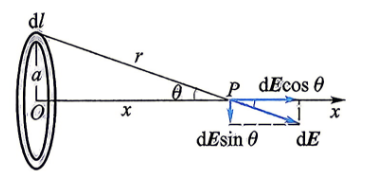
\includegraphics[width=0.3\linewidth]{figure/L7-2}
		\caption{例题L7-2辅助图}
		\label{fig:L7-2}
	\end{figure}
	
	\vspace{1em}
	
	\setcounter{equation}{0}
	\renewcommand{\theHequation}{L7-2.\arabic{equation}}
	
	\textbf{答案： }
	圆环轴线上与环心相距 $x$ 的 $P$ 点的场强大小为 $E = \frac{qx}{4\pi\varepsilon_0(a^2+x^2)^{3/2}}$，方向沿轴线（当 $q>0$ 时背离圆心向外，当 $q<0$ 时指向圆心）。
	
	\textbf{解答过程： }
	在圆环上任取一线元 $\mathrm{d}l$，由于电荷均匀分布，其上所带电荷量为：
	\begin{align*}
		\mathrm{d}q = \frac{q}{2\pi a} \mathrm{d}l
	\end{align*}
	该点电荷元在空间 $P$ 点产生的微场强大小为：
	\begin{equation}\label{eq:L7-2-1}
		\mathrm{d}E = \frac{1}{4\pi\varepsilon_0} \frac{\mathrm{d}q}{r^2} = \frac{1}{4\pi\varepsilon_0} \frac{\mathrm{d}q}{a^2+x^2}
	\end{equation}
	建立坐标系，设圆环轴线为 $x$ 轴。将 $\mathrm{d}E$ 分解为平行于轴线的分量 $\mathrm{d}E_x$ 和垂直于轴线的分量 $\mathrm{d}E_{\perp}$：
	\begin{align*}
		\mathrm{d}E_x &= \mathrm{d}E \cos\theta \\
		\mathrm{d}E_{\perp} &= \mathrm{d}E \sin\theta
	\end{align*}
	由圆环的空间对称性可知，对环上任意取定的一个电荷元 $\mathrm{d}q$，在环的直径相对端必存在一个等量电荷元。它们在 $P$ 点产生的垂直于轴线的分量大小相等、方向相反，相互抵消。因此，整个圆环在 $P$ 点产生的总场强的垂直分量积分为零：
	\begin{align*}
		E_{\perp} = \int \mathrm{d}E_{\perp} = 0
	\end{align*}
	所以，总场强即为平行于轴线的分量的积分。由几何关系可知 $\cos\theta = \frac{x}{r} = \frac{x}{\sqrt{a^2+x^2}}$，代入得到：
	\begin{equation}\label{eq:L7-2-2}
		E = \int \mathrm{d}E_x = \int \mathrm{d}E \cos\theta = \int \frac{1}{4\pi\varepsilon_0} \frac{\mathrm{d}q}{a^2+x^2} \frac{x}{\sqrt{a^2+x^2}}
	\end{equation}
	积分是沿着整个圆环进行的。在积分过程中，环上所有的电荷元到 $P$ 点的距离 $r$ 以及角度 $\theta$ 都是恒定的（即 $a$ 和 $x$ 对于积分变量 $\mathrm{d}q$ 是常量），因此可以将其全部提取到积分号外：
	\begin{align*}
		E &= \frac{x}{4\pi\varepsilon_0 (a^2+x^2)^{3/2}} \int \mathrm{d}q
	\end{align*}
	考虑到所有电荷元之和即为总电荷量 $\int \mathrm{d}q = q$，最终得到总场强为：
	\begin{equation}\label{eq:L7-2-3}
		E = \frac{qx}{4\pi\varepsilon_0 (a^2+x^2)^{3/2}}
	\end{equation}
	
	\textbf{易混淆知识点： }
	1. \textbf{积分常量的提取}：处理连续带电体场强时，很多人在面对积分号会感到迷茫。本题的核心在于识别出：在沿着圆环边缘遍历积分时，距离 $r$ 和角度 $\theta$ 并不随位置的改变而改变。将它们视作常量提出积分号外，复杂的矢量积分就瞬间转化为了求总电荷量 $q$ 的简单标量加法。
	
	2. \textbf{对称性的优先应用}：如果在此题中强行去积分垂直分量 $\mathrm{d}E_{\perp}$，不仅计算极其复杂且容易出错。\textcolor{red}{在电磁学中处理连续电荷分布问题时，“先找对称性”是第一原则。通过对称性直接判断出垂直分量抵消为零，可以省去一半以上的计算量。}
	
	3. \textbf{极值情况的物理检验}：推导出的公式可以通过极限情况来检验对错。例如：当 $x=0$ 时（考察点在环心处），由对称性显然可知场强相互抵消为0，代入公式 $E=0$ 符合预期；当 $x \gg a$ 时（距离极远），圆环可近似看作点电荷，公式分母的 $a^2$ 可忽略，退化为 $E \approx \frac{q}{4\pi\varepsilon_0 x^2}$，正好对应库仑定律。
	
	\vspace{2em}
	
	\item[\textbf{L7-5}]
	均匀带电球面的场强.设有一均匀带电球面,半径为$R$,电荷为$+q$,求球面内外任一点场强.
	
	
	\begin{figure}[H]
		\centering
		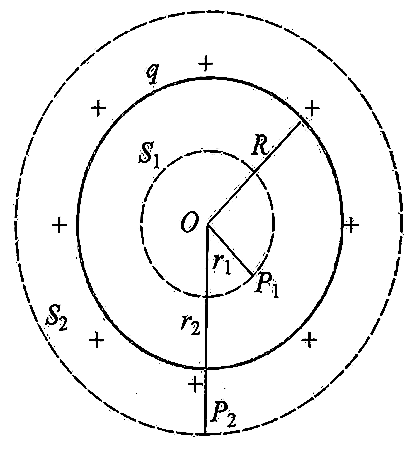
\includegraphics[width=0.3\linewidth]{figure/L7-5}
		\caption{例题L7-5辅助图}
		\label{fig:L7-5}
	\end{figure}
	
	\vspace{1em}
	
	\setcounter{equation}{0}
	\renewcommand{\theHequation}{L7-5.\arabic{equation}}
	
	\textbf{答案： }
	球面内任一点的场强为 $0$ ($r < R$)；\\
	球面外任一点的场强大小为 $E = \frac{q}{4\pi\varepsilon_0 r^2}$ ($r > R$)，方向沿径向向外。
	
	\textbf{解答过程： }
	由于电荷均匀分布在球面上，由空间对称性可知，产生的电场分布具有球对称性。即电场线必定沿径向，且在以球心 $O$ 为圆心、半径为 $r$ 的球面上，各点场强大小 $E$ 相等。
	
	根据高斯定理：
	\begin{equation}\label{eq:L7-5-1}
		\oint_S \vec{E} \cdot \mathrm{d}\vec{S} = \frac{1}{\varepsilon_0} \sum q_{\text{内}}
	\end{equation}
	
	(1) 求球面内任一点 $P_1$ 的场强（设距球心 $r_1 < R$）：
	过点 $P_1$ 作一半径为 $r_1$ 的同心球面 $S_1$ 作为闭合高斯面。由于电场强度方向垂直于高斯面且大小处处相等，高斯面上的电通量为：
	\begin{align*}
		\Phi_{e1} = \oint_{S_1} E \mathrm{d}S = E \cdot 4\pi r_1^2
	\end{align*}
	因为该高斯面完全在带电球面内部，其包围的净电荷量 $\sum q_{\text{内}} = 0$。代入高斯定理公式(\ref{eq:L7-5-1})得到：
	\begin{equation}\label{eq:L7-5-2}
		E \cdot 4\pi r_1^2 = 0
	\end{equation}
	由此解得，球面内各点场强为：
	\begin{equation}\label{eq:L7-5-3}
		E = 0 \quad (r < R)
	\end{equation}
	
	(2) 求球面外任一点 $P_2$ 的场强（设距球心 $r_2 > R$）：
	过点 $P_2$ 作一半径为 $r_2$ 的同心球面 $S_2$ 作为闭合高斯面。同理，高斯面上的电通量为：
	\begin{align*}
		\Phi_{e2} = \oint_{S_2} E \mathrm{d}S = E \cdot 4\pi r_2^2
	\end{align*}
	该高斯面将整个带电球面包围在内，因此其包围的总电荷量即为球面上携带的全部电荷，即 $\sum q_{\text{内}} = q$。代入高斯定理公式(\ref{eq:L7-5-1})得到：
	\begin{equation}\label{eq:L7-5-4}
		E \cdot 4\pi r_2^2 = \frac{q}{\varepsilon_0}
	\end{equation}
	由此解得，球面外各点场强大小为：
	\begin{equation}\label{eq:L7-5-5}
		E = \frac{q}{4\pi\varepsilon_0 r_2^2} \quad (r > R)
	\end{equation}
	因为带正电 ($+q$)，所以场强方向沿径向向外。可以发现，这与将全部电荷集中于球心的点电荷在外部空间产生的场强完全相同。
	
	\textbf{易混淆知识点： }
	1. \textbf{高斯面的选择原则}：\textcolor{red}{应用高斯定理计算场强的前提是}\textbf{电荷分布具有高度对称性（球对称、轴对称或面对称）。}通过构造与之匹配的对称高斯面，使得待求的 $E$ 可以作为常量提出积分号 $\oint E \mathrm{d}S = E \oint \mathrm{d}S = ES$，从而极大简化计算。
	
	2. \textbf{带电球面与实心球体的区别}：这是一个非常经典的易错点。\textbf{本题是“均匀带电球面”（如金属球壳），电荷只分布在表面，所以内部高斯面无法包围任何电荷，导致内部场强恒为零。}如果是均匀带电的绝缘“实心球体”（即体电荷分布），其内部高斯面会包围一部分电荷，内部场强就不为零，而是与半径 $r$ 成正比增大。
	
	3. \textbf{球面处场强的非连续性}：在 $r=R$ 处，场强发生突变。从内部无限逼近表面时场强为 $0$；从外部无限逼近表面时场强为 $\frac{q}{4\pi\varepsilon_0 R^2}$。这种由于表面电荷层导致的场强突变现象在静电学中非常普遍。
	
	\vspace{2em}
	
	\item[\textbf{L7-7}]
	无限长均匀带电圆柱面,半径为 $R$,电荷面密度 $\sigma>0$,求柱面内外任一点场强.
	
	\begin{figure}[H]
		\centering
		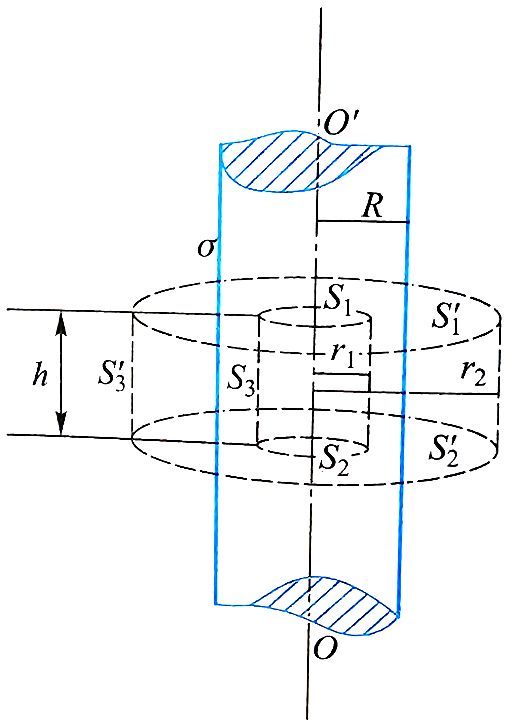
\includegraphics[width=0.3\linewidth]{figure/L7-7}
		\caption{例题L7-7辅助图}
		\label{fig:L7-7}
	\end{figure}
	
	\vspace{1em}
	
	\setcounter{equation}{0}
	\renewcommand{\theHequation}{L7-7.\arabic{equation}}
	
	\textbf{答案： }
	柱面内任一点的场强为 $0$ ($r < R$)；\\
	柱面外任一点的场强大小为 $E = \frac{\sigma R}{\varepsilon_0 r}$ ($r > R$)，方向垂直于圆柱轴线沿径向向外。
	
	\textbf{解答过程： }
	由于电荷均匀分布在无限长圆柱面上，由空间对称性可知，其产生的电场具有轴对称性。电场线必定垂直于圆柱轴线呈辐射状向外分布（因为 $\sigma > 0$），且在距离轴线为 $r$ 的同轴圆柱面上，各点场强大小 $E$ 相等。
	
	根据高斯定理：
	\begin{equation}\label{eq:L7-7-1}
		\oint_S \vec{E} \cdot \mathrm{d}\vec{S} = \frac{1}{\varepsilon_0} \sum q_{\text{内}}
	\end{equation}
	
	(1) 求柱面内任一点的场强（设距轴线距离为 $r_1 < R$）：
	取一段长为 $h$、半径为 $r_1$ 的同轴封闭圆柱面作为高斯面。该高斯面由上底面 $S_1$、下底面 $S_2$ 和侧面 $S_3$ 组成。
	\textbf{由于电场线平行于上下底面，穿过上下底面的电通量为 $0$。}电场线垂直穿过侧面，故穿过整个高斯面的总电通量仅为\textbf{侧面的电通量：}
	\begin{align*}
		\Phi_{e1} = \oint_{S} \vec{E} \cdot \mathrm{d}\vec{S} = \int_{S_3} E \mathrm{d}S = E \cdot 2\pi r_1 h
	\end{align*}
	因为该高斯面完全在带电圆柱面内部，其包围的净电荷量 $\sum q_{\text{内}} = 0$。代入高斯定理公式(\ref{eq:L7-7-1})得到：
	\begin{equation}\label{eq:L7-7-2}
		E \cdot 2\pi r_1 h = 0
	\end{equation}
	由此解得，柱面内各点场强为：
	\begin{equation}\label{eq:L7-7-3}
		E = 0 \quad (r < R)
	\end{equation}
	
	(2) 求柱面外任一点的场强（设距轴线距离为 $r_2 > R$）：
	取一段长为 $h$、半径为 $r_2$ 的同轴封闭圆柱面作为高斯面。\textbf{同理，穿过上下底面 $S'_1$、$S'_2$ 的电通量为 $0$}，总电通量即为穿过侧面 $S'_3$ 的电通量：
	\begin{align*}
		\Phi_{e2} = E \cdot 2\pi r_2 h
	\end{align*}
	该高斯面内部包围的电荷仅分布在半径为 $R$、长为 $h$ 的那一段真实带电圆柱面上。因此，高斯面内包围的总电荷量为：
	\begin{align*}
		\sum q_{\text{内}} = \sigma S_{\text{带电}} = \sigma \cdot 2\pi R h
	\end{align*}
	代入高斯定理公式(\ref{eq:L7-7-1})得到：
	\begin{equation}\label{eq:L7-7-4}
		E \cdot 2\pi r_2 h = \frac{\sigma \cdot 2\pi R h}{\varepsilon_0}
	\end{equation}
	化简解得，柱面外各点场强大小为：
	\begin{equation}\label{eq:L7-7-5}
		E = \frac{\sigma R}{\varepsilon_0 r_2} \quad (r > R)
	\end{equation}
	由于面电荷密度 $\sigma > 0$，场强方向垂直于圆柱轴线向外。
	
	\textbf{易混淆知识点： }
	1. \textbf{高斯面内包围电荷的计算}：在计算柱面外（$r_2 > R$）高斯面内的电荷时，\textcolor{red}{极易错误地将电荷量写为 $\sigma \cdot 2\pi r_2 h$}\textbf{。必须牢记，电荷只存在于真实的带电体（半径为 $R$ 的圆柱面）上，高斯面内部只有半径为 $R$ 的那部分柱面上有电荷，其余空间是真空。}
	
	2. \textbf{不同带电体场强的空间衰减规律}：对于无限大均匀带电平面，场强与距离无关（常数）；\textbf{对于无限长均匀带电直线或圆柱面，场强与距离成反比（$E \propto 1/r$）；对于点电荷或带电球面，场强与距离的平方成反比（$E \propto 1/r^2$）。}在检查推导结果时，可以通过量纲和距离的依赖关系来验证正确性。
	
	3. \textbf{圆柱面高斯面底面通量的处理}：必须在解答中明确指出，\textbf{之所以只计算侧面积的通量}，\textcolor{red}{是因为上下底面的法向量与电场方向垂直}，导致点积 $\vec{E} \cdot \mathrm{d}\vec{S} = 0$。如果跳过这一步直接写面积，不仅物理过程不完整，在考试中也极其容易丢掉步骤分。
	
	\vspace{2em}
	
	\item[\textbf{L7-9}]
	有两个厚度不计的平行无限大均匀带电平板 $A$、$B$,电荷面密度分别为
	\begin{enumerate}
		\item $+\sigma,\,+\sigma$；
		\item $+\sigma,\,-\sigma$.
	\end{enumerate}
	
	请分别求板内、外的场强.
	
	\begin{figure}[H]
		\centering
		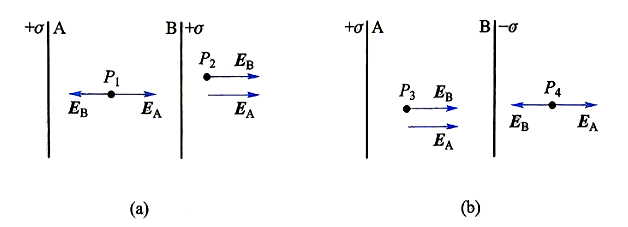
\includegraphics[width=0.5\linewidth]{figure/L7-9}
		\caption{例题L7-9辅助图}
		\label{fig:L7-9}
	\end{figure}
	
	\vspace{1em}
	

	\setcounter{equation}{0}
	\renewcommand{\theHequation}{L7-9.\arabic{equation}}
	
	\textbf{答案： }
	(1) 当电荷面密度分别为 $+\sigma, +\sigma$ 时，板内场强为 $0$；板外场强大小为 $\frac{\sigma}{\varepsilon_0}$，方向均背离两板向外。\\
	(2) 当电荷面密度分别为 $+\sigma, -\sigma$ 时，板内场强大小为 $\frac{\sigma}{\varepsilon_0}$，方向由正极板指向负极板；板外场强均为 $0$。
	
	\textbf{解答过程： }
	\textbf{由高斯定理可知}，无限大均匀带电平板在周围空间产生匀强电场，其场强大小与距板的距离无关，\textcolor{red}{单块平板产生的场强公式为}：
	\begin{equation}\label{eq:L7-9-1}
		E = \frac{|\sigma|}{2\varepsilon_0}
	\end{equation}
	电场方向：若平板带正电，场强方向背离极板；若平板带负电，场强方向指向极板。
	
	设向右为正方向。平板 $A$ 位于左侧，平板 $B$ 位于右侧。根据场强叠加原理，空间任一点的总场强为：
	\begin{equation}\label{eq:L7-9-2}
		\vec{E} = \vec{E}_A + \vec{E}_B
	\end{equation}
	
	(1) 当两板电荷面密度均为 $+\sigma$ 时：
	板 $A$ 和板 $B$ 均带正电，在空间各点产生的场强大小均为 $E_A = E_B = \frac{\sigma}{2\varepsilon_0}$。
	
	\textbf{在板内（两板之间）}：$\vec{E}_A$ 偏向右，$\vec{E}_B$ 偏向左，两者方向相反。
	\begin{align*}
		E_{\text{内}} = E_A - E_B = \frac{\sigma}{2\varepsilon_0} - \frac{\sigma}{2\varepsilon_0} = 0
	\end{align*}
	
	\textbf{在板外（两板外侧）}：
	在板 $A$ 左侧，$\vec{E}_A$ 和 $\vec{E}_B$ 均向左，总场强大小为 $E_{\text{外左}} = \frac{\sigma}{2\varepsilon_0} + \frac{\sigma}{2\varepsilon_0} = \frac{\sigma}{\varepsilon_0}$，方向向左。
	在板 $B$ 右侧，$\vec{E}_A$ 和 $\vec{E}_B$ 均向右，总场强大小为 $E_{\text{外右}} = \frac{\sigma}{2\varepsilon_0} + \frac{\sigma}{2\varepsilon_0} = \frac{\sigma}{\varepsilon_0}$，方向向右。
	综上，板外场强大小为 $\frac{\sigma}{\varepsilon_0}$，方向均背离两板向外。
	
	(2) 当两板电荷面密度分别为 $+\sigma, -\sigma$ 时（即平行板电容器模型）：
	板 $A$ 带正电，板 $B$ 带负电。它们在空间产生的场强大小仍均为 $E_A = E_B = \frac{\sigma}{2\varepsilon_0}$。
	
	\textbf{在板内（两板之间）}：$\vec{E}_A$ 背离板 $A$ 向右，$\vec{E}_B$ 指向板 $B$ 也向右，两者方向相同。
	\begin{align*}
		E_{\text{内}} = E_A + E_B = \frac{\sigma}{2\varepsilon_0} + \frac{\sigma}{2\varepsilon_0} = \frac{\sigma}{\varepsilon_0}
	\end{align*}
	方向向右（由带正电的板 $A$ 垂直指向带负电的板 $B$）。
	
	\textbf{在板外（两板外侧）}：
	在板 $A$ 左侧，$\vec{E}_A$ 向左，$\vec{E}_B$ 向右，两者相互抵消，总场强 $E_{\text{外左}} = 0$。
	在板 $B$ 右侧，$\vec{E}_A$ 向右，$\vec{E}_B$ 向左，两者相互抵消，总场强 $E_{\text{外右}} = 0$。
	综上，板外场强均为 $0$。
	
	\textbf{易混淆知识点： }
	1. \textbf{公式分母的常数}：\textcolor{red}{无限大均匀带电“几何面”（厚度不计）的场强公式是 $\frac{\sigma}{2\varepsilon_0}$。}许多人会将其与带电“导体板”表面附近的场强公式 $\frac{\sigma}{\varepsilon_0}$ 混淆。\textbf{本题明确指明是“厚度不计的平板”，相当于一层电荷面，因此必须使用 $\frac{\sigma}{2\varepsilon_0}$。}
	
	2. \textbf{场强与距离无关}：\textcolor{red}{由高斯定理推导出的无限大平面场强是一个常数，与考察点到平面的距离完全无关。}因此，即使考察点距离板 $A$ 近、距离板 $B$ 远，\textbf{在进行矢量叠加时，两者贡献的场强大小绝对值依然是相等的。}(带绝对值的原因.)
	
	3. \textbf{平行板电容器的物理模型}：第(2)问的计算结果（内部为 $\frac{\sigma}{\varepsilon_0}$，外部为 $0$）正是理想平行板电容器内部为匀强电场、外部无漏电场的理论基础。
	
	\vspace{2em}
	
	\item[\textbf{L7-11}]
	一个均匀带电球面,半径为 $R$,电荷为 $q$,求球面内、外任一点电势.
	
	\begin{figure}[H]
		\centering
		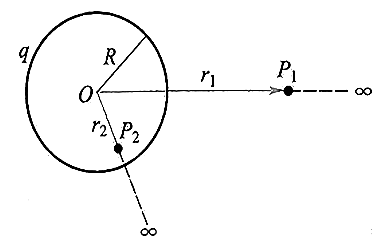
\includegraphics[width=0.5\linewidth]{figure/L7-11}
		\caption{例题L7-11辅助图}
		\label{fig:L7-11}
	\end{figure}
	
	\vspace{1em}
	
	\setcounter{equation}{0}
	\renewcommand{\theHequation}{L7-11.\arabic{equation}}
	
	\textbf{答案： }
	球面内任一点的电势为 $V = \frac{q}{4\pi\varepsilon_0 R}$ ($r \le R$)；\\
	球面外任一点的电势为 $V = \frac{q}{4\pi\varepsilon_0 r}$ ($r > R$)。
	
	\textbf{解答过程： }
	已知均匀带电球面产生的电场分布为：
	球面外 ($x > R$) 的场强：
	\begin{equation}\label{eq:L7-11-1}
		E_{\text{外}} = \frac{q}{4\pi\varepsilon_0 x^2}
	\end{equation}
	球面内 ($x < R$) 的场强：
	\begin{equation}\label{eq:L7-11-2}
		E_{\text{内}} = 0
	\end{equation}
	规定无限远处为电势零点。根据电势的定义，空间距球心为 $r$ 处某点的电势 $V$ 等于将单位正电荷从该点移至无限远处的过程中电场力所作的功：
	\begin{align*}
		V = \int_{r}^{\infty} E \mathrm{d}x
	\end{align*}
	
	(1) 当考察点在球面外 ($r > R$) 时，积分路径上只有球面外的电场：
	\begin{align*}
		V &= \int_{r}^{\infty} E_{\text{外}} \mathrm{d}x \\
		&= \int_{r}^{\infty} \frac{q}{4\pi\varepsilon_0 x^2} \mathrm{d}x
	\end{align*}
	计算定积分得到球面外的电势：
	\begin{equation}\label{eq:L7-11-3}
		V = \frac{q}{4\pi\varepsilon_0 r} \quad (r > R)
	\end{equation}
	
	(2) \textcolor{red}{当考察点在球面内 ($r < R$) 时，积分路径必须分为两段：从 $r$ 到 $R$（处于球面内），以及从 $R$ 到无限远（处于球面外）}：
	\begin{align*}
		V &= \int_{r}^{R} E_{\text{内}} \mathrm{d}x + \int_{R}^{\infty} E_{\text{外}} \mathrm{d}x \\
		&= \int_{r}^{R} 0 \mathrm{d}x + \int_{R}^{\infty} \frac{q}{4\pi\varepsilon_0 x^2} \mathrm{d}x
	\end{align*}
	\textbf{第一段路径上电场为零，积分为 $0$；第二段积分等同于球面表面的电势：}
	\begin{equation}\label{eq:L7-11-4}
		V = 0 + \frac{q}{4\pi\varepsilon_0 R} = \frac{q}{4\pi\varepsilon_0 R} \quad (r \le R)
	\end{equation}
	
	\textbf{易混淆知识点： }
	1. \textbf{内部电场为零不等于电势为零}：很多人误以为带电球面内部场强 $E=0$，所以电势 $V=0$。\textbf{实际上，电场为零只代表内部各点之间没有电势差，即内部是一个等势体。}\textcolor{red}{其内部的电势值由边界（球表面）决定，处处等于表面的电势常数。}
	
	2. \textbf{积分路径的分段}：在计算球面内部某点的电势时，必须将向外的积分路径在半径 $R$ 处截断分为两段。\textbf{因为在 $R$ 的内外两侧，空间电场的分布函数是完全不同的，不能用同一个公式一积到底。}
	
	3. \textbf{场强突变与电势连续}：\textbf{电场强度}在带电球面表面 ($r=R$) 处\textbf{发生突变}（从内侧的 $0$ 瞬间跳跃到外侧的 $\frac{q}{4\pi\varepsilon_0 R^2}$），\textcolor{red}{但电势在整个空间（包括表面）是连续过渡的}。将 $r=R$ 分别代入内外电势公式，得到的数值是相等的。
	
	\vspace{2em}
	
	\item[\textbf{L7-12}]
	如图L7-12所示,有两个均匀带电的同心球面,半径分别为 $R_1$、$R_2$,电荷分别为 $+q$、$-q$,求两球面的电势差 $U$.
	
	\begin{figure}[H]
		\centering
		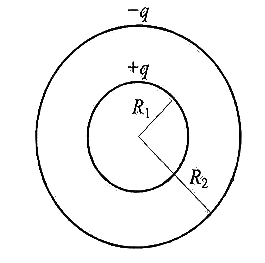
\includegraphics[width=0.4\linewidth]{figure/L7-12}
		\caption{例题L7-12图}
		\label{fig:L7-12}
	\end{figure}
	
	\vspace{1em}
	
	\setcounter{equation}{0}
	\renewcommand{\theHequation}{L7-12.\arabic{equation}}
	
	\textbf{答案： }
	两球面的电势差为 $U = \frac{q}{4\pi\varepsilon_0} \left( \frac{1}{R_1} - \frac{1}{R_2} \right)$。
	
	\textbf{解答过程： }
	
	\textbf{方法一：电场积分法}
	根据高斯定理，在两同心球面之间的区域（径向距离 $R_1 < r < R_2$），作一半径为 $r$ 的同心球面作为闭合高斯面。该高斯面内部包围的净电荷仅为内球面的电荷 $+q$（外球面电荷均匀分布，在其内部 $r < R_2$ 空间产生的场强处处为零）。
	由高斯定理 $\oint \vec{E} \cdot \mathrm{d}\vec{S} = \frac{\sum q_{\text{内}}}{\varepsilon_0}$，得到两球面间区域的电场强度大小为：
	\begin{equation}\label{eq:L7-12-1}
		E = \frac{q}{4\pi\varepsilon_0 r^2}
	\end{equation}
	方向沿径向向外。
	根据电势差的定义，两球面的电势差 $U = V_1 - V_2$ 等于将单位正电荷从内球面移至外球面时电场力所作的功：
	\begin{align*}
		U &= \int_{R_1}^{R_2} \vec{E} \cdot \mathrm{d}\vec{r} \\
		&= \int_{R_1}^{R_2} \frac{q}{4\pi\varepsilon_0 r^2} \mathrm{d}r
	\end{align*}
	计算该定积分：
	\begin{equation}\label{eq:L7-12-2}
		U = \frac{q}{4\pi\varepsilon_0} \left[ -\frac{1}{r} \right]_{R_1}^{R_2} = \frac{q}{4\pi\varepsilon_0} \left( \frac{1}{R_1} - \frac{1}{R_2} \right)
	\end{equation}
	
	\textbf{方法二：电势叠加法}
	空间中任意一点的电势，等于内外两个带电球面单独存在时在该点产生电势的代数和。
	设无穷远处为电势零点。
	内球面（半径 $R_1$，电荷 $+q$）产生的电势分布：在其内部为 $\frac{q}{4\pi\varepsilon_0 R_1}$，在其外部为 $\frac{q}{4\pi\varepsilon_0 r}$。
	外球面（半径 $R_2$，电荷 $-q$）产生的电势分布：在其内部为 $\frac{-q}{4\pi\varepsilon_0 R_2}$，在其外部为 $\frac{-q}{4\pi\varepsilon_0 r}$。
	内球面上的电势 $V_1$（此时距球心 $r = R_1$，对内球面在表面，对外球面在内部）：
	\begin{equation}\label{eq:L7-12-3}
		V_1 = \frac{q}{4\pi\varepsilon_0 R_1} + \frac{-q}{4\pi\varepsilon_0 R_2}
	\end{equation}
	外球面上的电势 $V_2$（此时距球心 $r = R_2$，对内球面在外部，对外球面在表面）：
	\begin{equation}\label{eq:L7-12-4}
		V_2 = \frac{q}{4\pi\varepsilon_0 R_2} + \frac{-q}{4\pi\varepsilon_0 R_2} = 0
	\end{equation}
	因此，两球面的电势差为：
	\begin{align*}
		U &= V_1 - V_2 \\
		&= \left( \frac{q}{4\pi\varepsilon_0 R_1} - \frac{q}{4\pi\varepsilon_0 R_2} \right) - 0 \\
		&= \frac{q}{4\pi\varepsilon_0} \left( \frac{1}{R_1} - \frac{1}{R_2} \right)
	\end{align*}
	
	\textbf{易混淆知识点： }
	1. \textbf{高斯面内包围电荷的误判}：在利用方法一求两球面间的电场时，许多人会不自觉地将外球面的电荷 $-q$ 也一并代入高斯定理。实际上，根据高斯面的几何位置（$R_1 < r < R_2$），它仅仅包围了内球面的 $+q$，外球面的电荷在它的外面，对穿过该高斯面的净电通量毫无贡献。
	
	2. \textbf{球壳内部电势并非为零}：在使用方法二叠加电势时，必须牢记均匀带电球壳在其内部产生的电场虽然为零，但内部的电势是一个非零常量（处处等于其表面的电势）。外球面在内球面处（$r=R_1$）贡献的电势是 $\frac{-q}{4\pi\varepsilon_0 R_2}$，而不是 $0$ 或 $\frac{-q}{4\pi\varepsilon_0 R_1}$。
	
	3. \textbf{电容器模型的静电屏蔽效应}：计算结果显示外球面电势 $V_2 = 0$，这意味着如果把外球面接地，系统的电荷分布和内外电势差依然保持不变。这是一个典型的球形电容器模型，所有的电场线都起始于内球面并全部终止于外球面的内侧，外部空间完全没有电场（静电屏蔽）。
	
\end{enumerate}

\newpage

\subsection{第八章}

\begin{enumerate}
	
	\item[\textbf{L8-1}]
	半径为$a$的两平行长直导线相距为$d$（$d$远远大于$a$）,二者电荷线密度为$+\lambda$、$-\lambda$,试求：
	
	\begin{figure}[H]
		\centering
		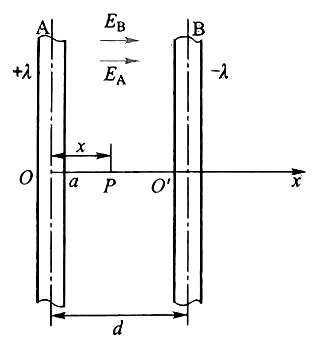
\includegraphics[width=0.3\linewidth]{figure/L8-1}
		\caption{例题L8-1辅助图}
		\label{fig:L8-1}
	\end{figure}
	
	
	\begin{enumerate}
		\item 两导线间电势差；
		\item 此导线组单位长度的电容.
	\end{enumerate}
	
	\vspace{1em}
	
	\setcounter{equation}{0}
	\renewcommand{\theHequation}{L8-1.\arabic{equation}}
	
	\textbf{答案： }
	(1) 两导线间电势差为 $U \approx \frac{\lambda}{\pi\varepsilon_0} \ln\frac{d}{a}$ （精确值为 $U = \frac{\lambda}{\pi\varepsilon_0} \ln\frac{d-a}{a}$）。\\
	(2) 此导线组单位长度的电容为 $C_0 \approx \frac{\pi\varepsilon_0}{\ln\frac{d}{a}}$ （精确值为 $C_0 = \frac{\pi\varepsilon_0}{\ln\frac{d-a}{a}}$）。
	
	\textbf{解答过程： }
	(1) 设想两导线带有等量异号电荷，线电荷密度分别为 $+\lambda$ 和 $-\lambda$。
	根据高斯定理，无限长均匀带电直导线在距离为 $r$ 处产生的电场强度大小为：
	\begin{align*}
		E = \frac{\lambda}{2\pi\varepsilon_0 r}
	\end{align*}
	建立如图所示的坐标系，原点 $O$ 位于左侧正极导线轴线上，$x$ 轴垂直于导线向右。
	在两导线之间（$a \le x \le d-a$），\textbf{左侧正导线产生的电场 $E_A$ 向右，右侧负导线产生的电场 $E_B$ 也向右。}根据电场叠加原理，两导线连线上的总电场为：
	\begin{equation}\label{eq:L8-1-1}
		E = E_A + E_B = \frac{\lambda}{2\pi\varepsilon_0 x} + \frac{\lambda}{2\pi\varepsilon_0 (d-x)}
	\end{equation}
	两导线间的电势差 $U$ 等于将单位正电荷从正极板表面（$x=a$）移至负极板表面（$x=d-a$）时电场力所做的功：
	\begin{align*}
		U &= \int_{a}^{d-a} E \mathrm{d}x \\
		&= \int_{a}^{d-a} \frac{\lambda}{2\pi\varepsilon_0} \left( \frac{1}{x} + \frac{1}{d-x} \right) \mathrm{d}x \\
		&= \frac{\lambda}{2\pi\varepsilon_0} \left[ \ln x - \ln(d-x) \right]_{a}^{d-a} \\
		&= \frac{\lambda}{2\pi\varepsilon_0} \left( (\ln(d-a) - \ln a) - (\ln a - \ln(d-a)) \right) \\
		&= \frac{\lambda}{2\pi\varepsilon_0} \left( 2\ln(d-a) - 2\ln a \right)
	\end{align*}
	化简得到精确的电势差表达式：
	\begin{equation}\label{eq:L8-1-2}
		U = \frac{\lambda}{\pi\varepsilon_0} \ln\frac{d-a}{a}
	\end{equation}
	考虑到题目给定的条件 $d \gg a$，可作近似 $d-a \approx d$，则有：
	\begin{equation}\label{eq:L8-1-3}
		U \approx \frac{\lambda}{\pi\varepsilon_0} \ln\frac{d}{a}
	\end{equation}
	
	(2) 设导线的长度为 $l$，则所带电荷量为 $Q = \lambda l$。
	该导线组构成的平行双线电容器的总电容为：
	\begin{align*}
		C = \frac{Q}{U} = \frac{\lambda l}{U}
	\end{align*}
	单位长度的电容 $C_0$ 为：
	\begin{equation}\label{eq:L8-1-4}
		C_0 = \frac{C}{l} = \frac{\lambda}{U}
	\end{equation}
	将近似电势差公式(\ref{eq:L8-1-3})代入公式(\ref{eq:L8-1-4})中，得到：
	\begin{equation}\label{eq:L8-1-5}
		C_0 \approx \frac{\pi\varepsilon_0}{\ln\frac{d}{a}}
	\end{equation}
	（若要求精确值，代入公式(\ref{eq:L8-1-2})则为 $C_0 = \frac{\pi\varepsilon_0}{\ln\frac{d-a}{a}}$）
	
	\textbf{易混淆知识点： }
	1. \textbf{电势差积分的上下限}：计算两导线间的电势差时，\textcolor{red}{积分必须从一个导体的\textbf{表面}积到另一个导体的\textbf{表面}（即从 $a$ 到 $d-a$）}。\textbf{绝对不能从轴心积到轴心（从 $0$ 到 $d$），}因为在理想线电荷模型中，$r=0$ 处电场趋于无穷大，积分会发散。\textbf{由于导体是等势体，其内部没有电势差，}电势变化全部集中在它们外部的真空区域。
	
	2. \textbf{两电场矢量的叠加方向}：虽然两根导线带异号电荷，但在它们之间的区域，\textbf{正电荷产生的电场排斥向右，负电荷产生的电场吸引也向右。}所以总电场是二者大小\textbf{相加}（$\frac{1}{x} + \frac{1}{d-x}$），而不是相减。
	
	3. \textbf{远大于条件的使用}：题目特意加上“$d$ 远远大于 $a$”的条件，\textbf{正是为了在对数项中进行近似化简（$\frac{d-a}{a} \approx \frac{d}{a}$）。}在处理实际工程中的平行双线传输线时，这种近似非常普遍且足够精确。
	
	\vspace{2em}
	
	\item[\textbf{L8-2}]
	有一个带电为 $+q$、半径为 $R_1$ 的导体球,与内外半径分别为 $R_3, R_4$、带电荷为 $-q$ 的导体球壳同心,两者之间有两层均匀电介质,内层和外层电介质的电容率分别为 $\varepsilon_1, \varepsilon_2$,且两电介质分界面也是与导体球同心的半径为 $R_2$ 的球面.试求：
	
	\begin{enumerate}
		\item 电位移分布；
		\item 场强分布；
		\item 导体球与导体球壳间的电势差；
		\item 导体球壳构成电容器的电容.
	\end{enumerate}
	
	\begin{figure}[H]
		\centering
		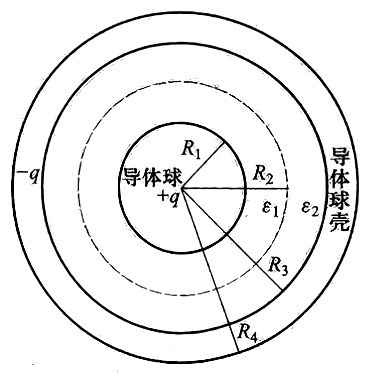
\includegraphics[width=0.3\linewidth]{figure/L8-2}
		\caption{例题L8-2辅助图}
		\label{fig:L8-2}
	\end{figure}
	
	\vspace{1em}
	
	\setcounter{equation}{0}
	\renewcommand{\theHequation}{L8-2.\arabic{equation}}
	
	\textbf{答案： }
	(1) 电位移分布为：在 $R_1 < r < R_3$ 区域，大小为 $D = \frac{q}{4\pi r^2}$；在其他区域（$r < R_1$ 及 $r > R_3$），$D = 0$。方向均沿径向向外。\\
	(2) 场强分布为：在 $R_1 < r < R_2$ 区域，$E_1 = \frac{q}{4\pi\varepsilon_1 r^2}$；在 $R_2 < r < R_3$ 区域，$E_2 = \frac{q}{4\pi\varepsilon_2 r^2}$；在其他区域，$E = 0$。方向均沿径向向外。\\
	(3) 导体球与导体球壳间的电势差为 $U = \frac{q}{4\pi} \left[ \frac{1}{\varepsilon_1}\left(\frac{1}{R_1} - \frac{1}{R_2}\right) + \frac{1}{\varepsilon_2}\left(\frac{1}{R_2} - \frac{1}{R_3}\right) \right]$。\\
	(4) 该电容器的电容为 $C = \frac{4\pi}{\frac{1}{\varepsilon_1}\left(\frac{1}{R_1} - \frac{1}{R_2}\right) + \frac{1}{\varepsilon_2}\left(\frac{1}{R_2} - \frac{1}{R_3}\right)}$。
	
	\textbf{解答过程： }
	(1) 这是一个具有球对称性的静电场问题，由于存在电介质，我们首先应用有电介质时的高斯定理（介质高斯定理）来求解电位移矢量 $\vec{D}$：
	\begin{equation}\label{eq:L8-2-1}
		\oint \vec{D} \cdot \mathrm{d}\vec{S} = \sum q_{\text{内0}}
	\end{equation}
	其中 $\sum q_{\text{内0}}$ 为高斯面内包围的自由电荷代数和。
	作一半径为 $r$ 的同心球面作为高斯面：
	- 当 $r < R_1$ 时，高斯面在导体球内部，内部自由电荷为零且静电平衡，故 $D = 0$。
	- 当 $R_1 < r < R_3$ 时，高斯面位于电介质中，其包围的自由电荷仅为内层导体球上的 $+q$。由高斯定理有：
	\begin{align*}
		D \cdot 4\pi r^2 = q
	\end{align*}
	解得电位移大小为：
	\begin{equation}\label{eq:L8-2-2}
		D = \frac{q}{4\pi r^2} \quad (R_1 < r < R_3)
	\end{equation}
	注意：这个结果表明 $\vec{D}$ 的分布只与自由电荷有关，在两层不同电介质的分界面（$r = R_2$）上，由于没有自由电荷，$\vec{D}$ 是连续的。
	- 当 $R_3 < r < R_4$ 时，高斯面在导体球壳内部，处于静电平衡状态，场强为零，故 $D = 0$。
	- 当 $r > R_4$ 时，高斯面包围的总自由电荷为 $+q + (-q) = 0$，故 $D = 0$。
	
	(2) 利用电位移与电场强度的本构关系 $\vec{D} = \varepsilon \vec{E}$，即可求得空间各区域的电场强度大小：
	- 在第一层电介质中（$R_1 < r < R_2$），介电常数为 $\varepsilon_1$：
	\begin{equation}\label{eq:L8-2-3}
		E_1 = \frac{D}{\varepsilon_1} = \frac{q}{4\pi\varepsilon_1 r^2}
	\end{equation}
	- 在第二层电介质中（$R_2 < r < R_3$），介电常数为 $\varepsilon_2$：
	\begin{equation}\label{eq:L8-2-4}
		E_2 = \frac{D}{\varepsilon_2} = \frac{q}{4\pi\varepsilon_2 r^2}
	\end{equation}
	- 在导体内及球壳外部，由于 $D=0$，场强 $E=0$。
	
	(3) 导体球（正极）与导体球壳（负极）之间的电势差 $U$ 等于电场强度沿径向从内球积分到外球的线积分。由于空间中存在两层不同的电场分布，积分需要分段进行：
	\begin{align*}
		U &= \int_{R_1}^{R_3} E \mathrm{d}r \\
		&= \int_{R_1}^{R_2} E_1 \mathrm{d}r + \int_{R_2}^{R_3} E_2 \mathrm{d}r \\
		&= \int_{R_1}^{R_2} \frac{q}{4\pi\varepsilon_1 r^2} \mathrm{d}r + \int_{R_2}^{R_3} \frac{q}{4\pi\varepsilon_2 r^2} \mathrm{d}r
	\end{align*}
	分别计算定积分：
	\begin{equation}\label{eq:L8-2-5}
		U = \frac{q}{4\pi\varepsilon_1} \left( \frac{1}{R_1} - \frac{1}{R_2} \right) + \frac{q}{4\pi\varepsilon_2} \left( \frac{1}{R_2} - \frac{1}{R_3} \right)
	\end{equation}
	
	(4) 根据电容的定义式 $C = \frac{Q}{U}$，将求得的电势差代入，得到该球形电容器的总电容：
	\begin{equation}\label{eq:L8-2-6}
		C = \frac{q}{U} = \frac{4\pi}{\frac{1}{\varepsilon_1}\left(\frac{1}{R_1} - \frac{1}{R_2}\right) + \frac{1}{\varepsilon_2}\left(\frac{1}{R_2} - \frac{1}{R_3}\right)}
	\end{equation}
	
	\textbf{易混淆知识点： }
	1. \textbf{$\vec{D}$ 与 $\vec{E}$ 连续性的区别}：在处理多层电介质问题时，这是最核心的考点。电位移矢量 $\vec{D}$ 的分布仅仅取决于“自由电荷”。因为两层介质分界面（$r=R_2$）上没有自由电荷，所以 $\vec{D}$ 是穿过界面连续变化的。然而，由于极化产生的束缚电荷积累在界面上，电场强度 $\vec{E} = \vec{D}/\varepsilon$ 会因为介电常数的不同而在此界面处发生“阶跃突变”。
	
	2. \textbf{串联电容器模型的等效思想}：这个多层介质球形电容器实际上可以等效为两个单层介质球形电容器的“串联”。内层（$R_1$ 到 $R_2$）电容 $C_1 = \frac{4\pi\varepsilon_1}{\frac{1}{R_1} - \frac{1}{R_2}}$，外层（$R_2$ 到 $R_3$）电容 $C_2 = \frac{4\pi\varepsilon_2}{\frac{1}{R_2} - \frac{1}{R_3}}$。由第(4)问的最终结果可以看出，它完美符合串联电容公式 $\frac{1}{C} = \frac{1}{C_1} + \frac{1}{C_2}$，利用这种等效物理图景可以快速检验计算结果的正确性。
	
	3. \textbf{介电常数符号的使用}：题目给出的是各介质层的绝对介电常数（也称电容率） $\varepsilon_1$ 和 $\varepsilon_2$，而不是相对介电常数 $\varepsilon_r$。所以在公式中不需要再额外乘以真空介电常数 $\varepsilon_0$。若题目给出的是相对介电常数，则分母需写为 $\varepsilon_0 \varepsilon_{r1}$ 等。

\end{enumerate}

\newpage

\subsection{第九章}
\begin{enumerate}
	\item 
\end{enumerate}

\newpage

\subsection{第十章}
\begin{enumerate}
	\item 
\end{enumerate}

\newpage

\subsection{第十一章}
\begin{enumerate}
	\item 
\end{enumerate}












